\documentclass[]{book}
\usepackage{lmodern}
\usepackage{amssymb,amsmath}
\usepackage{ifxetex,ifluatex}
\usepackage{fixltx2e} % provides \textsubscript
\ifnum 0\ifxetex 1\fi\ifluatex 1\fi=0 % if pdftex
  \usepackage[T1]{fontenc}
  \usepackage[utf8]{inputenc}
\else % if luatex or xelatex
  \ifxetex
    \usepackage{mathspec}
  \else
    \usepackage{fontspec}
  \fi
  \defaultfontfeatures{Ligatures=TeX,Scale=MatchLowercase}
\fi
% use upquote if available, for straight quotes in verbatim environments
\IfFileExists{upquote.sty}{\usepackage{upquote}}{}
% use microtype if available
\IfFileExists{microtype.sty}{%
\usepackage{microtype}
\UseMicrotypeSet[protrusion]{basicmath} % disable protrusion for tt fonts
}{}
\usepackage{hyperref}
\hypersetup{unicode=true,
            pdftitle={Learning statistics with R},
            pdfauthor={Danielle Navarro},
            pdfborder={0 0 0},
            breaklinks=true}
\urlstyle{same}  % don't use monospace font for urls
\usepackage{natbib}
\bibliographystyle{apalike}
\usepackage{color}
\usepackage{fancyvrb}
\newcommand{\VerbBar}{|}
\newcommand{\VERB}{\Verb[commandchars=\\\{\}]}
\DefineVerbatimEnvironment{Highlighting}{Verbatim}{commandchars=\\\{\}}
% Add ',fontsize=\small' for more characters per line
\usepackage{framed}
\definecolor{shadecolor}{RGB}{248,248,248}
\newenvironment{Shaded}{\begin{snugshade}}{\end{snugshade}}
\newcommand{\AlertTok}[1]{\textcolor[rgb]{0.94,0.16,0.16}{#1}}
\newcommand{\AnnotationTok}[1]{\textcolor[rgb]{0.56,0.35,0.01}{\textbf{\textit{#1}}}}
\newcommand{\AttributeTok}[1]{\textcolor[rgb]{0.77,0.63,0.00}{#1}}
\newcommand{\BaseNTok}[1]{\textcolor[rgb]{0.00,0.00,0.81}{#1}}
\newcommand{\BuiltInTok}[1]{#1}
\newcommand{\CharTok}[1]{\textcolor[rgb]{0.31,0.60,0.02}{#1}}
\newcommand{\CommentTok}[1]{\textcolor[rgb]{0.56,0.35,0.01}{\textit{#1}}}
\newcommand{\CommentVarTok}[1]{\textcolor[rgb]{0.56,0.35,0.01}{\textbf{\textit{#1}}}}
\newcommand{\ConstantTok}[1]{\textcolor[rgb]{0.00,0.00,0.00}{#1}}
\newcommand{\ControlFlowTok}[1]{\textcolor[rgb]{0.13,0.29,0.53}{\textbf{#1}}}
\newcommand{\DataTypeTok}[1]{\textcolor[rgb]{0.13,0.29,0.53}{#1}}
\newcommand{\DecValTok}[1]{\textcolor[rgb]{0.00,0.00,0.81}{#1}}
\newcommand{\DocumentationTok}[1]{\textcolor[rgb]{0.56,0.35,0.01}{\textbf{\textit{#1}}}}
\newcommand{\ErrorTok}[1]{\textcolor[rgb]{0.64,0.00,0.00}{\textbf{#1}}}
\newcommand{\ExtensionTok}[1]{#1}
\newcommand{\FloatTok}[1]{\textcolor[rgb]{0.00,0.00,0.81}{#1}}
\newcommand{\FunctionTok}[1]{\textcolor[rgb]{0.00,0.00,0.00}{#1}}
\newcommand{\ImportTok}[1]{#1}
\newcommand{\InformationTok}[1]{\textcolor[rgb]{0.56,0.35,0.01}{\textbf{\textit{#1}}}}
\newcommand{\KeywordTok}[1]{\textcolor[rgb]{0.13,0.29,0.53}{\textbf{#1}}}
\newcommand{\NormalTok}[1]{#1}
\newcommand{\OperatorTok}[1]{\textcolor[rgb]{0.81,0.36,0.00}{\textbf{#1}}}
\newcommand{\OtherTok}[1]{\textcolor[rgb]{0.56,0.35,0.01}{#1}}
\newcommand{\PreprocessorTok}[1]{\textcolor[rgb]{0.56,0.35,0.01}{\textit{#1}}}
\newcommand{\RegionMarkerTok}[1]{#1}
\newcommand{\SpecialCharTok}[1]{\textcolor[rgb]{0.00,0.00,0.00}{#1}}
\newcommand{\SpecialStringTok}[1]{\textcolor[rgb]{0.31,0.60,0.02}{#1}}
\newcommand{\StringTok}[1]{\textcolor[rgb]{0.31,0.60,0.02}{#1}}
\newcommand{\VariableTok}[1]{\textcolor[rgb]{0.00,0.00,0.00}{#1}}
\newcommand{\VerbatimStringTok}[1]{\textcolor[rgb]{0.31,0.60,0.02}{#1}}
\newcommand{\WarningTok}[1]{\textcolor[rgb]{0.56,0.35,0.01}{\textbf{\textit{#1}}}}
\usepackage{longtable,booktabs}
\usepackage{graphicx,grffile}
\makeatletter
\def\maxwidth{\ifdim\Gin@nat@width>\linewidth\linewidth\else\Gin@nat@width\fi}
\def\maxheight{\ifdim\Gin@nat@height>\textheight\textheight\else\Gin@nat@height\fi}
\makeatother
% Scale images if necessary, so that they will not overflow the page
% margins by default, and it is still possible to overwrite the defaults
% using explicit options in \includegraphics[width, height, ...]{}
\setkeys{Gin}{width=\maxwidth,height=\maxheight,keepaspectratio}
\IfFileExists{parskip.sty}{%
\usepackage{parskip}
}{% else
\setlength{\parindent}{0pt}
\setlength{\parskip}{6pt plus 2pt minus 1pt}
}
\setlength{\emergencystretch}{3em}  % prevent overfull lines
\providecommand{\tightlist}{%
  \setlength{\itemsep}{0pt}\setlength{\parskip}{0pt}}
\setcounter{secnumdepth}{5}
% Redefines (sub)paragraphs to behave more like sections
\ifx\paragraph\undefined\else
\let\oldparagraph\paragraph
\renewcommand{\paragraph}[1]{\oldparagraph{#1}\mbox{}}
\fi
\ifx\subparagraph\undefined\else
\let\oldsubparagraph\subparagraph
\renewcommand{\subparagraph}[1]{\oldsubparagraph{#1}\mbox{}}
\fi

%%% Use protect on footnotes to avoid problems with footnotes in titles
\let\rmarkdownfootnote\footnote%
\def\footnote{\protect\rmarkdownfootnote}

%%% Change title format to be more compact
\usepackage{titling}

% Create subtitle command for use in maketitle
\providecommand{\subtitle}[1]{
  \posttitle{
    \begin{center}\large#1\end{center}
    }
}

\setlength{\droptitle}{-2em}

  \title{Learning statistics with R}
    \pretitle{\vspace{\droptitle}\centering\huge}
  \posttitle{\par}
    \author{Danielle Navarro}
    \preauthor{\centering\large\emph}
  \postauthor{\par}
      \predate{\centering\large\emph}
  \postdate{\par}
    \date{14 July 2019}

\usepackage{booktabs}

\begin{document}
\maketitle

{
\setcounter{tocdepth}{1}
\tableofcontents
}
\hypertarget{preface}{%
\chapter*{Preface}\label{preface}}
\addcontentsline{toc}{chapter}{Preface}

This is a book. It contains things. Lots of exciting things.

\hypertarget{part-getting-started}{%
\part{Getting started}\label{part-getting-started}}

\hypertarget{intro}{%
\chapter{Introduction}\label{intro}}

\hypertarget{whywhywhy}{%
\section{Why statistics?}\label{whywhywhy}}

To the surprise of many students, statistics is large part of a psychological education. To the surprise of no-one, statistics is very rarely the \emph{favourite} part of one's psychological education. After all, if you really loved the idea of doing statistics, you'd probably be enrolled in a statistics class right now, not a psychology class. So, not surprisingly, there's a pretty large proportion of the student base that isn't happy about the fact that psychology has so much statistics in it. In view of this, I thought that the right place to start might be to answer some of the more common questions that people have about stats\ldots{}

A big part of this issue at hand relates to the very idea of statistics. What is it? What's it there for? And why are scientists so bloody obsessed with it? These are all good questions, when you think about it. So let's start with the last one. As a group, scientists seem to be bizarrely fixated on running statistical tests on everything. In fact, we use statistics so often that we sometimes forget to explain to people why we do. It's a kind of article of faith among scientists -- and especially social scientists -- that your findings can't be trusted until you've done some stats. Undergraduate students might be forgiven for thinking that we're all completely mad, because no-one takes the time to answer one very simple question: *Why do we do statistics? Why don't scientists just use **common sense?*

It's a naive question in some ways, but most good questions are. There are many good answers to the question but perhaps the best one is the simplest one: we don't trust ourselves enough. We worry that we're human, and susceptible to all of the biases, temptations and frailties that humans suffer from. Statistics provides us with tools to help us understand our data, but it also provides us with safeguards. Using common sense to evaluate evidence means trusting ``gut instincts'', relying on verbal arguments and on using the raw power of human reason to come up with the right answer. As smart as we are as humans, we aren't perfect, and if we want to avoid innocent self-deception, we need something a little more rigorous.

In fact, come to think of it, this sounds a lot like a psychological question to me, and since I do work in a psychology department, it seems like a good idea to dig a little deeper here. Is it really plausible to think that this ``common sense'' approach is very trustworthy? Verbal arguments have to be constructed in language, and all languages have biases -- some things are harder to say than others, and not necessarily because they're false (e.g., quantum electrodynamics is a good theory, but hard to explain in words). The instincts of our ``gut'' aren't designed to solve scientific problems, they're designed to handle day to day inferences -- and given that biological evolution is slower than cultural change, we should say that they're designed to solve the day to day problems for a \emph{different world} than the one we live in. Most fundamentally, reasoning sensibly requires people to engage in ``induction'', making wise guesses and going beyond the immediate evidence of the senses to make generalisations about the world. If you think that you can do that without being influenced by various distractors, well, I have a bridge in Brooklyn I'd like to sell you. Heck, as the next section shows, we can't even solve ``deductive'' problems (ones where no guessing is required) without being influenced by our pre-existing biases.

\hypertarget{the-parable-of-belief-bias}{%
\section{The parable of belief bias}\label{the-parable-of-belief-bias}}

People are mostly pretty smart. We're certainly smarter than the other species that we share the planet with (though many people might disagree). Our minds are quite amazing things, and we seem to be capable of the most incredible feats of thought and reason. That doesn't make us perfect though. And among the many things that psychologists have shown over the years is that we really do find it hard to be neutral, to evaluate evidence impartially and without being swayed by pre-existing biases. A good example of this is the \textbf{\emph{belief bias effect}} in logical reasoning: if you ask people to decide whether a particular argument is logically valid (i.e., conclusion would be true if the premises were true), we tend to be influenced by the believability of the conclusion, even when we shouldn't. For instance, here's a valid argument where the conclusion is believable:

\begin{quote}
No cigarettes are inexpensive (Premise 1)\\
Some addictive things are inexpensive (Premise 2)\\
Therefore, some addictive things are not cigarettes (Conclusion)
\end{quote}

And here's a valid argument where the conclusion is not believable:

\begin{quote}
No addictive things are inexpensive (Premise 1)\\
Some cigarettes are inexpensive (Premise 2)\\
Therefore, some cigarettes are not addictive (Conclusion)
\end{quote}

The logical \emph{structure} of argument \#2 is identical to the structure of argument \#1, and they're both valid. However, in the second argument, there are good reasons to think that premise 1 is incorrect, and as a result it's probably the case that the conclusion is also incorrect. But that's entirely irrelevant to the topic at hand: an argument is deductively valid if the conclusion is a logical consequence of the premises. That is, a valid argument doesn't have to involve true statements.

On the other hand, here's an invalid argument that has a believable conclusion:

\begin{quote}
No addictive things are inexpensive (Premise 1)\\
Some cigarettes are inexpensive (Premise 2)\\
Therefore, some addictive things are not cigarettes (Conclusion)
\end{quote}

And finally, an invalid argument with an unbelievable conclusion:

\begin{quote}
No cigarettes are inexpensive (Premise 1)\\
Some addictive things are inexpensive (Premise 2)\\
Therefore, some cigarettes are not addictive (Conclusion)
\end{quote}

Now, suppose that people really are perfectly able to set aside their pre-existing biases about what is true and what isn't, and purely evaluate an argument on its logical merits. We'd expect 100\% of people to say that the valid arguments are valid, and 0\% of people to say that the invalid arguments are valid. So if you ran an experiment looking at this, you'd expect to see data like this:

\begin{longtable}[]{@{}lcc@{}}
\toprule
& conclusion feels true & conclusion feels false\tabularnewline
\midrule
\endhead
argument is valid & 100\% say ``valid'' & 100\% say ``valid''\tabularnewline
argument is invalid & 0\% say ``valid'' & 0\% say ``valid''\tabularnewline
\bottomrule
\end{longtable}

If the psychological data looked like this (or even a good approximation to this), we might feel safe in just trusting our gut instincts. That is, it'd be perfectly okay just to let scientists evaluate data based on their common sense, and not bother with all this murky statistics stuff. However, you guys have taken psych classes, and by now you probably know where this is going\ldots{}

In a classic study, EVANS ran an experiment looking at exactly this. What they found is that when pre-existing biases (i.e., beliefs) were in agreement with the structure of the data, everything went the way you'd hope:

\begin{longtable}[]{@{}lcc@{}}
\toprule
& conclusion feels true & conclusion feels false\tabularnewline
\midrule
\endhead
argument is valid & 92\% say ``valid'' &\tabularnewline
argument is invalid & & 8\% say ``valid''\tabularnewline
\bottomrule
\end{longtable}

Not perfect, but that's pretty good. But look what happens when our intuitive feelings about the truth of the conclusion run against the logical structure of the argument:

\begin{longtable}[]{@{}lcc@{}}
\toprule
& conclusion feels true & conclusion feels false\tabularnewline
\midrule
\endhead
argument is valid & 92\% say ``valid'' & \textbf{46\% say ``valid''}\tabularnewline
argument is invalid & \textbf{92\% say ``valid''} & 8\% say ``valid''\tabularnewline
\bottomrule
\end{longtable}

Oh dear, that's not as good. Apparently, when people are presented with a strong argument that contradicts our pre-existing beliefs, we find it pretty hard to even perceive it to be a strong argument (people only did so 46\% of the time). Even worse, when people are presented with a weak argument that agrees with our pre-existing biases, almost no-one can see that the argument is weak (people got that one wrong 92\% of the time!)\footnote{In my more cynical moments I feel like this fact alone explains 95\% of what I read on the internet.}

If you think about it, it's not as if these data are horribly damning. Overall, people did do better than chance at compensating for their prior biases, since about 60\% of people's judgements were correct (you'd expect 50\% by chance). Even so, if you were a professional ``evaluator of evidence'', and someone came along and offered you a magic tool that improves your chances of making the right decision from 60\% to (say) 95\%, you'd probably jump at it, right? Of course you would. Thankfully, we actually do have a tool that can do this. But it's not magic, it's statistics. So that's reason \#1 why scientists love statistics. It's just \emph{too easy} for us to ``believe what we want to believe''; so if we want to ``believe in the data'' instead, we're going to need a bit of help to keep our personal biases under control. That's what statistics does: it helps keep us honest.

\hypertarget{statistics-in-psychology}{%
\section{Statistics in psychology}\label{statistics-in-psychology}}

I hope that the discussion above helped explain why science in general is so focused on statistics. But I'm guessing that you have a lot more questions about what role statistics plays in psychology, and specifically why psychology classes always devote so many lectures to stats. So here's my attempt to answer a few of them\ldots{}

\textbf{Why does psychology have so much statistics?}

To be perfectly honest, there's a few different reasons, some of which are better than others. The most important reason is that psychology is a statistical science. What I mean by that is that the ``things'' that we study are \emph{people}. Real, complicated, gloriously messy, infuriatingly perverse people. The ``things'' of physics include object like electrons, and while there are all sorts of complexities that arise in physics, electrons don't have minds of their own. They don't have opinions, they don't differ from each other in weird and arbitrary ways, they don't get bored in the middle of an experiment, and they don't get angry at the experimenter and then deliberately try to sabotage the data set (not that I've ever done that\ldots{}). At a fundamental level psychology is harder than physics.\footnote{Which might explain why physics is just a teensy bit further advanced as a science than we are.}

Basically, we teach statistics to you as psychologists because you need to be better at stats than physicists. There's actually a saying used sometimes in physics, to the effect that ``if your experiment needs statistics, you should have done a better experiment''. They have the luxury of being able to say that because their objects of study are pathetically simple in comparison to the vast mess that confronts social scientists. It's not just psychology, really: most social sciences are desperately reliant on statistics. Not because we're bad experimenters, but because we've picked a harder problem to solve. We teach you stats because you really, really need it.

\textbf{Can't someone else do the statistics?}

To some extent, but not completely. It's true that you don't need to become a fully trained statistician just to do psychology, but you do need to reach a certain level of statistical competence. In my view, there's three reasons that every psychological researcher ought to be able to do basic statistics:

\begin{itemize}
\tightlist
\item
  Firstly, there's the fundamental reason: statistics is deeply intertwined with research design. If you want to be good at designing psychological studies, you need to at least understand the basics of stats.
\item
  Secondly, if you want to be good at the psychological side of the research, then you need to be able to understand the psychological literature, right? But almost every paper in the psychological literature reports the results of statistical analyses. So if you really want to understand the psychology, you need to be able to understand what other people did with their data. And that means understanding a certain amount of statistics.
\item
  Thirdly, there's a big practical problem with being dependent on other people to do all your statistics: statistical analysis is \emph{expensive}. If you ever get bored and want to look up how much the Australian government charges for university fees, you'll notice something interesting: statistics is designated as a ``national priority'' category, and so the fees are much, much lower than for any other area of study. This is because there's a massive shortage of statisticians out there. So, from your perspective as a psychological researcher, the laws of supply and demand aren't exactly on your side here! As a result, in almost any real life situation where you want to do psychological research, the cruel facts will be that you don't have enough money to afford a statistician. So the economics of the situation mean that you have to be pretty self-sufficient.
\end{itemize}

Note that a lot of these reasons generalise beyond researchers. If you want to be a practicing psychologist and stay on top of the field, it helps to be able to read the scientific literature, which relies pretty heavily on statistics.

\textbf{I don't care about jobs, research, or clinical work. Do I need statistics?}

Okay, now you're just messing with me. Still, I think it should matter to you too. Statistics should matter to you in the same way that statistics should matter to \emph{everyone}: we live in the 21st century, and data are \emph{everywhere}. Frankly, given the world in which we live these days, a basic knowledge of statistics is pretty damn close to a survival tool! Which is the topic of the next section\ldots{}

\hypertarget{statistics-in-everyday-life}{%
\section{Statistics in everyday life}\label{statistics-in-everyday-life}}

\begin{quote}
\emph{``We are drowning in information,~but we are starved for knowledge''}

-Various authors, original probably John Naisbitt
\end{quote}

When I started writing up my lecture notes I took the 20 most recent news articles posted to the ABC news website. Of those 20 articles, it turned out that 8 of them involved a discussion of something that I would call a statistical topic; 6 of those made a mistake. The most common error, if you're curious, was failing to report baseline data (e.g., the article mentions that 5\% of people in situation X have some characteristic Y, but doesn't say how common the characteristic is for everyone else!) The point I'm trying to make here isn't that journalists are bad at statistics (though they sometimes are), it's that a basic knowledge of statistics is very helpful for trying to figure out when someone else is either making a mistake or even lying to you.

\hypertarget{on-the-limitations-of-statistics}{%
\section{On the limitations of statistics}\label{on-the-limitations-of-statistics}}

Before leaving this topic entirely, I want to point out something else really critical that is often overlooked in a research methods class. Statistics only solves \emph{part} of the problem. Remember that we started all this with the concern that Berkeley's admissions processes might be unfairly biased against female applicants. When we looked at the ``aggregated'' data, it did seem like the university was discriminating against women, but when we ``disaggregate'' and looked at the individual behaviour of all the departments, it turned out that the actual departments were, if anything, slightly biased in favour of women. The gender bias in total admissions was caused by the fact that women tended to self-select for harder departments. From a legal perspective, that would probably put the university in the clear. Postgraduate admissions are determined at the level of the individual department (and there are good reasons to do that), and at the level of individual departments, the decisions are more or less unbiased (the weak bias in favour of females at that level is small, and not consistent across departments). Since the university can't dictate which departments people choose to apply to, and the decision making takes place at the level of the department it can hardly be held accountable for any biases that those choices produce.

That was the basis for my somewhat glib remarks earlier, but that's not exactly the whole story, is it? After all, if we're interested in this from a more sociological and psychological perspective, we might want to ask \emph{why} there are such strong gender differences in applications. Why do males tend to apply to engineering more often than females, and why is this reversed for the English department? And why is it it the case that the departments that tend to have a female-application bias tend to have lower overall admission rates than those departments that have a male-application bias? Might this not still reflect a gender bias, even though every single department is itself unbiased? It might. Suppose, hypothetically, that males preferred to apply to ``hard sciences'' and females prefer ``humanities''. And suppose further that the reason for why the humanities departments have low admission rates is because the government doesn't want to fund the humanities (Ph.D.~places, for instance, are often tied to government funded research projects). Does that constitute a gender bias? Or just an unenlightened view of the value of the humanities? What if someone at a high level in the government cut the humanities funds because they felt that the humanities are ``useless chick stuff''. That seems pretty \emph{blatantly} gender biased. None of this falls within the purview of statistics, but it matters to the research project. If you're interested in the overall structural effects of subtle gender biases, then you probably want to look at \emph{both} the aggregated and disaggregated data. If you're interested in the decision making process at Berkeley itself then you're probably only interested in the disaggregated data.

In short there are a lot of critical questions that you can't answer with statistics, but the answers to those questions will have a huge impact on how you analyse and interpret data. And this is the reason why you should always think of statistics as a \emph{tool} to help you learn about your data, no more and no less. It's a powerful tool to that end, but there's no substitute for careful thought.

So far, most of what I've talked about is statistics, and so you'd be forgiven for thinking that statistics is all I care about in life. To be fair, you wouldn't be far wrong, but research methodology is a broader concept than statistics. So most research methods courses will cover a lot of topics that relate much more to the pragmatics of research design, and in particular the issues that you encounter when trying to do research with humans. However, about 99\% of student \emph{fears} relate to the statistics part of the course, so I've focused on the stats in this discussion, and hopefully I've convinced you that statistics matters, and more importantly, that it's not to be feared. That being said, it's pretty typical for introductory research methods classes to be very stats-heavy. This is not (usually) because the lecturers are evil people. Quite the contrary, in fact. Introductory classes focus a lot on the statistics because you almost always find yourself needing statistics before you need the other research methods training. Why? Because almost all of your assignments in other classes will rely on statistical training, to a much greater extent than they rely on other methodological tools. It's not common for undergraduate assignments to require you to design your own study from the ground up (in which case you would need to know a lot about research design), but it \emph{is} common for assignments to ask you to analyse and interpret data that were collected in a study that someone else designed (in which case you need statistics). In that sense, from the perspective of allowing you to do well in all your other classes, the statistics is more urgent.

But note that ``urgent'' is different from ``important'' -- they both matter. I really do want to stress that research design is just as important as data analysis, and this book does spend a fair amount of time on it. However, while statistics has a kind of universality, and provides a set of core tools that are useful for most types of psychological research, the research methods side isn't quite so universal. There are some general principles that everyone should think about, but a lot of research design is very idiosyncratic, and is specific to the area of research that you want to engage in. To the extent that it's the details that matter, those details don't usually show up in an introductory stats and research methods class.

\hypertarget{r-start}{%
\chapter{Getting started in R}\label{r-start}}

\begin{quote}
Machine dreams hold a special vertigo.
~~~~~~--William Gibson, \emph{Count Zero}, 1986
\end{quote}

In this chapter I'll discuss how to get started in R. I'll briefly talk about how to download and install R, then show you how to write R commands. The goal in this chapter is not to learn any statistical or programming concepts: we're just trying to learn how R works and get comfortable interacting with the system. We'll spend a bit of time using R as a simple calculator, since that's the easiest thing to do with R, just to give you a feel for what it's like to work in R.

\hypertarget{why-learn-r}{%
\section{Why learn R?}\label{why-learn-r}}

\hypertarget{first-steps}{%
\section{First steps}\label{first-steps}}

\hypertarget{installing-r-rstudio}{%
\subsection{Installing R \& RStudio}\label{installing-r-rstudio}}

An important distinction to remember is between the R \emph{programming language} itself, and the software you use to interact with R. You could choose to interact with R directly from the terminal, but that's painful, so most people use an \emph{integrated development environment} (IDE), which takes care of a lot of boring tasks for you. For this class, we'll use the popular Rstudio IDE. To get started, make sure you have both R and RStudio installed on your computer. Both are free and open source, and for most people they should be straightforward to install.

\begin{itemize}
\item
  \textbf{Installing R}: Go to the \href{https://www.r-project.org/}{R website} and download the installer file. Once downloaded, open the installer file and follow the instructions.
\item
  \textbf{Installing RStudio}: Go to the \href{https://www.rstudio.com/}{R studio} website, and follow the links to download RStudio. The version you want is the ``RStudio Desktop''. Once the installer is downloaded, open it and follow the instructions.
\end{itemize}

To get started, open the \textbf{Rstudio} application (i.e., RStudio.exe or RStudio.app), not the vanilla application (i.e., not R.exe or R.app). You should be looking at something like this:

In the bottom left hand corner you'll see a panel labelled \emph{Console}, and a whole lot of text that doesn't make much sense. Ignore it for now! The important part is this\ldots{}

\begin{verbatim}
>
\end{verbatim}

\ldots{} which has a flashing cursor next to it. That's the \emph{command prompt}. When you see this, it means that R is waiting patiently for you to do something! So it's time to get started!

\hypertarget{r-commands}{%
\subsection{R commands}\label{r-commands}}

One of the easiest things you can do with R is use it as a simple calculator, so it's a good place to start. For instance, try typing 30, and hitting enter. When you do this, you've entered a command, and R will \textbf{execute} that command. What you see on screen now will be this:

\begin{Shaded}
\begin{Highlighting}[]
\DecValTok{10} \OperatorTok{+}\StringTok{ }\DecValTok{20}
\end{Highlighting}
\end{Shaded}

\begin{verbatim}
## [1] 30
\end{verbatim}

Not a lot of surprises in this extract. But there's a few things worth talking about, even with such a simple example. Firstly, it's important that you understand how to read the extract. In this example, what I typed was the \texttt{10\ +\ 20} part at the top, and the content below is what R produced.

Secondly, it's important to understand how the output is formatted. When you look at the output on your screen it will probably look like this \texttt{{[}1{]}\ 30}. Obviously, the correct answer to the sum \texttt{10\ +\ 20} is \texttt{30}, and not surprisingly R has printed that out as part of its response. But it's also printed out this \texttt{{[}1{]}} part, which probably doesn't make a lot of sense to you right now. You're going to see that a lot. I'll talk about what this means in a bit more detail later on, but for now you can think of \texttt{{[}1{]}} 30 as if R were saying ``the answer to the first question you asked is 30''. That's not quite the truth, but it's close enough for now. And in any case it's not really very interesting at the moment: we only asked R to calculate one thing, so obviously there's only one answer printed on the screen. Later on this will change, and the \texttt{{[}1{]}} part will start to make a bit more sense. For now, I just don't want you to get confused or concerned by it.

\hypertarget{avoid-typos}{%
\subsection{Avoid typos}\label{avoid-typos}}

Before we go on to talk about other types of calculations that we can do with R, there's a few other things I want to point out. The first thing is that, while R is good software, it's still software. It's pretty stupid, and because it's stupid it can't handle typos. It takes it on faith that you meant to type exactly what you did type. For example, suppose that you forgot to hit the shift key when trying to type \texttt{+}, and as a result your command ended up being \texttt{10\ =\ 20} rather than \texttt{10\ +\ 20}. Here's what happens:

\begin{Shaded}
\begin{Highlighting}[]
\DecValTok{10}\NormalTok{ =}\StringTok{ }\DecValTok{20}
\end{Highlighting}
\end{Shaded}

\begin{verbatim}
## Error in 10 = 20: invalid (do_set) left-hand side to assignment
\end{verbatim}

What's happened here is that R has attempted to interpret \texttt{10\ =\ 20} as a command, and spits out an error message because the command doesn't make any sense to it. When a human looks at this, and then looks down at his or her keyboard and sees that + and = are on the same key, it's pretty obvious that the command was a typo. But R doesn't know this, so it gets upset. And, if you look at it from its perspective, this makes sense. All that R ``knows'' is that \texttt{10} is a legitimate number, \texttt{20} is a legitimate number, and \texttt{=} is a legitimate part of the language too. In other words, from its perspective this really does look like the user meant to type \texttt{10\ =\ 20}, since all the individual parts of that statement are legitimate and it's too stupid to realise that this is probably a typo. Therefore, R takes it on faith that this is exactly what you meant\ldots{} it only ``discovers'' that the command is nonsense when it tries to follow your instructions, typo and all. And then it whinges, and spits out an error.

Even more subtle is the fact that some typos won't produce errors at all, because they happen to correspond to ``well-formed'' R commands. For instance, suppose that not only did I forget to hit the shift key when trying to type \texttt{10\ +\ 20}, I also managed to press the key next to one I meant do. The resulting typo would produce the command \texttt{10\ -\ 20}. Clearly, R has no way of knowing that you meant to add \texttt{20} to \texttt{10}, not subtract \texttt{20} from \texttt{10}, so what happens this time is this:

\begin{Shaded}
\begin{Highlighting}[]
\DecValTok{10} \OperatorTok{-}\StringTok{ }\DecValTok{20}
\end{Highlighting}
\end{Shaded}

\begin{verbatim}
## [1] -10
\end{verbatim}

In this case, R produces the right answer, but to the the wrong question.

To some extent, I'm stating the obvious here, but it's important. The people who wrote R are smart. You, the user, are smart. But R itself is dumb. And because it's dumb, it has to be mindlessly obedient. It does exactly what you ask it to do. There is no equivalent to ``autocorrect'' in R, and for good reason. When doing advanced stuff -- and even the simplest of statistics is pretty advanced in a lot of ways -- it's dangerous to let a mindless automaton like R try to overrule the human user. But because of this, it's your responsibility to be careful. Always make sure you type exactly what you mean. When dealing with computers, it's not enough to type ``approximately'' the right thing. In general, you absolutely must be precise in what you say to R \ldots{} like all machines it is too stupid to be anything other than absurdly literal in its interpretation.

\hypertarget{r-is-flexible-with-spacing}{%
\subsection{R is flexible with spacing?}\label{r-is-flexible-with-spacing}}

Of course, now that I've been so uptight about the importance of always being precise, I should point out that there are some exceptions. Or, more accurately, there are some situations in which R does show a bit more flexibility than my previous description suggests. The first thing R is smart enough to do is ignore redundant spacing. What I mean by this is that, when I typed \texttt{10\ +\ 20} before, I could equally have done this

\begin{Shaded}
\begin{Highlighting}[]
\DecValTok{10}        \OperatorTok{+}\StringTok{ }\DecValTok{20}
\end{Highlighting}
\end{Shaded}

\begin{verbatim}
## [1] 30
\end{verbatim}

and get exactly the same answer. However, that doesn't mean that you can insert spaces in any old place. For instance, when you open up R it suggests that you type \texttt{citation()} to get some information about how to cite R:

\begin{Shaded}
\begin{Highlighting}[]
\KeywordTok{citation}\NormalTok{()}
\end{Highlighting}
\end{Shaded}

\begin{verbatim}
## 
## To cite R in publications use:
## 
##   R Core Team (2019). R: A language and environment for
##   statistical computing. R Foundation for Statistical Computing,
##   Vienna, Austria. URL https://www.R-project.org/.
## 
## A BibTeX entry for LaTeX users is
## 
##   @Manual{,
##     title = {R: A Language and Environment for Statistical Computing},
##     author = {{R Core Team}},
##     organization = {R Foundation for Statistical Computing},
##     address = {Vienna, Austria},
##     year = {2019},
##     url = {https://www.R-project.org/},
##   }
## 
## We have invested a lot of time and effort in creating R, please
## cite it when using it for data analysis. See also
## 'citation("pkgname")' for citing R packages.
\end{verbatim}

Okay, that's good to know. Let's see what happens when I try changing the spacing. If I insert spaces in between the word and the parentheses, or inside the parentheses themselves, then all is well. But insertinhg spaces in the middle of the commands, not so much. Try these three just to see:

\begin{Shaded}
\begin{Highlighting}[]
\KeywordTok{citation}\NormalTok{ ()     }\CommentTok{# works!}
\KeywordTok{citation}\NormalTok{(    )  }\CommentTok{# works!}
\NormalTok{cita }\KeywordTok{tion}\NormalTok{()     }\CommentTok{# doesn't work}
\end{Highlighting}
\end{Shaded}

\hypertarget{r-knows-youre-not-finished}{%
\subsection{R knows you're not finished?}\label{r-knows-youre-not-finished}}

One more thing I should point out. If you hit enter in a situation where it's ``obvious'' to R that you haven't actually finished typing the command, R is just smart enough to keep waiting. For example, if you type \texttt{10\ +} and then press enter, even R is smart enough to realise that you probably wanted to type in another number. So here's what happens:

\begin{verbatim}
> 10 +
+
\end{verbatim}

and there's a blinking cursor next to the plus sign. What this means is that R is still waiting for you to finish. It ``thinks'' you're still typing your command, so it hasn't tried to execute it yet. In other words, this plus sign is actually another command prompt. It's different from the usual one (i.e., the \texttt{\textgreater{}} symbol) to remind you that R is going to ``add'' whatever you type now to what you typed last time. For example, if I then go on to type \texttt{20} and hit enter, what I get is this:

\begin{verbatim}
> 10 +
+ 20
[1] 30
\end{verbatim}

And as far as R is concerned, this is exactly the same as if you had typed \texttt{10\ +\ 20}. Similarly, consider the \texttt{citation()} command that we talked about in the previous section. Suppose you hit enter after typing \texttt{citation(}. Once again, R is smart enough to realise that there must be more coming -- since you need to add the \texttt{)} character -- so it waits. I can even hit enter several times and it will keep waiting:

\begin{verbatim}
> citation( 
+
+
+)
\end{verbatim}

Sometimes when doing this, you'll eventually get yourself in trouble (it happens to us all). Maybe you start typing a command, and then you realise you've screwed up. For example,

\begin{verbatim}
> citblation(
+
+
\end{verbatim}

You'd probably prefer R not to try running this command, right? If you want to get out of this situation, just hit the \emph{escape} key. R will return you to the normal command prompt (i.e. \texttt{\textgreater{}}) without attempting to execute the botched command.

That being said, it's not often the case that R is smart enough to tell that there's more coming. For instance, in the same way that I can't add a space in the middle of a word, I can't hit enter in the middle of a word either. If I hit enter after typing \texttt{citat} I get an error, because R thinks I'm interested in something called \texttt{citat} and can't find it:

\begin{Shaded}
\begin{Highlighting}[]
\NormalTok{citat}
\end{Highlighting}
\end{Shaded}

\begin{verbatim}
## Error in eval(expr, envir, enclos): object 'citat' not found
\end{verbatim}

What about if I typed \texttt{citation} and hit enter, without the parentheses? In this case we get something very odd, something that we definitely don't want, at least not at this stage. Here's what happens:

\begin{Shaded}
\begin{Highlighting}[]
\NormalTok{citation}
\end{Highlighting}
\end{Shaded}

\begin{verbatim}
## function (package = "base", lib.loc = NULL, auto = NULL) 
## {
##     if (!is.null(auto) && !is.logical(auto) && !any(is.na(match(c("Package", 
##         "Version", "Title"), names(meta <- as.list(auto))))) && 
##         !all(is.na(match(c("Authors@R", "Author"), names(meta))))) {
##         auto_was_meta <- TRUE
##         package <- meta$Package
##     }
##     else {
##         auto_was_meta <- FALSE
##         dir <- system.file(package = package, lib.loc = lib.loc)
##         if (dir == "") 
##             stop(packageNotFoundError(package, lib.loc, sys.call()))
##         meta <- packageDescription(pkg = package, lib.loc = dirname(dir))
##         citfile <- file.path(dir, "CITATION")
##         test <- file_test("-f", citfile)
##         if (!test) {
##             citfile <- file.path(dir, "inst", "CITATION")
##             test <- file_test("-f", citfile)
##         }
##         if (is.null(auto)) 
##             auto <- !test
##         if (!auto) {
##             return(readCitationFile(citfile, meta))
##         }
##     }
##     if ((!is.null(meta$Priority)) && (meta$Priority == "base")) {
##         cit <- citation("base", auto = FALSE)
##         attr(cit, "mheader")[1L] <- paste0("The ", sQuote(package), 
##             " package is part of R.  ", attr(cit, "mheader")[1L])
##         return(.citation(cit, package))
##     }
##     year <- sub("-.*", "", meta$`Date/Publication`)
##     if (!length(year)) {
##         if (is.null(meta$Date)) {
##             warning(gettextf("no date field in DESCRIPTION file of package %s", 
##                 sQuote(package)), domain = NA)
##         }
##         else {
##             date <- trimws(as.vector(meta$Date))[1L]
##             date <- strptime(date, "%Y-%m-%d", tz = "GMT")
##             if (!is.na(date)) 
##                 year <- format(date, "%Y")
##         }
##     }
##     if (!length(year)) {
##         date <- as.POSIXlt(sub(";.*", "", trimws(meta$Packaged)[1L]))
##         if (!is.na(date)) 
##             year <- format(date, "%Y")
##     }
##     if (!length(year)) {
##         warning(gettextf("could not determine year for %s from package DESCRIPTION file", 
##             sQuote(package)), domain = NA)
##         year <- NA_character_
##     }
##     author <- meta$`Authors@R`
##     if (length(author)) {
##         aar <- .read_authors_at_R_field(author)
##         author <- Filter(function(e) {
##             !(is.null(e$given) && is.null(e$family)) && !is.na(match("aut", 
##                 e$role))
##         }, aar)
##         if (!length(author)) 
##             author <- Filter(function(e) {
##                 !(is.null(e$given) && is.null(e$family)) && !is.na(match("cre", 
##                   e$role))
##             }, aar)
##     }
##     if (length(author)) {
##         has_authors_at_R_field <- TRUE
##     }
##     else {
##         has_authors_at_R_field <- FALSE
##         author <- as.personList(meta$Author)
##     }
##     z <- list(title = paste0(package, ": ", meta$Title), author = author, 
##         year = year, note = paste("R package version", meta$Version))
##     if (identical(meta$Repository, "CRAN")) 
##         z$url <- sprintf("https://CRAN.R-project.org/package=%s", 
##             package)
##     if (identical(meta$Repository, "R-Forge")) {
##         z$url <- if (!is.null(rfp <- meta$"Repository/R-Forge/Project")) 
##             sprintf("https://R-Forge.R-project.org/projects/%s/", 
##                 rfp)
##         else "https://R-Forge.R-project.org/"
##         if (!is.null(rfr <- meta$"Repository/R-Forge/Revision")) 
##             z$note <- paste(z$note, rfr, sep = "/r")
##     }
##     if (!length(z$url) && !is.null(url <- meta$URL)) {
##         if (grepl("[, ]", url)) 
##             z$note <- url
##         else z$url <- url
##     }
##     header <- if (!auto_was_meta) {
##         gettextf("To cite package %s in publications use:", sQuote(package))
##     }
##     else NULL
##     footer <- if (!has_authors_at_R_field && !auto_was_meta) {
##         gettextf("ATTENTION: This citation information has been auto-generated from the package DESCRIPTION file and may need manual editing, see %s.", 
##             sQuote("help(\"citation\")"))
##     }
##     else NULL
##     author <- format(z$author, include = c("given", "family"))
##     if (length(author) > 1L) 
##         author <- paste(paste(head(author, -1L), collapse = ", "), 
##             tail(author, 1L), sep = " and ")
##     rval <- bibentry(bibtype = "Manual", textVersion = paste0(author, 
##         " (", z$year, "). ", z$title, ". ", z$note, ". ", z$url), 
##         header = header, footer = footer, other = z)
##     .citation(rval, package)
## }
## <bytecode: 0x55ca81f28980>
## <environment: namespace:utils>
\end{verbatim}

where the \texttt{BLAH\ BLAH\ BLAH} goes on for rather a long time, and you don't know enough R yet to understand what all this gibberish actually means. This incomprehensible output can be quite intimidating to novice users, and unfortunately it's very easy to forget to type the parentheses; so almost certainly you'll do this by accident. Do not panic when this happens. Simply ignore the gibberish.

\hypertarget{operations}{%
\section{Operations}\label{operations}}

Okay, now that we've discussed some of the tedious details associated with typing R commands, let's get back to learning how to use the most powerful piece of statistical software in the world as a \$2 calculator. So far, all we know how to do is addition. Clearly, a calculator that only did addition would be a bit stupid, so I should tell you about how to perform other simple calculations using R. But first, some more terminology. Addition is an example of an ``operation'' that you can perform (specifically, an arithmetic operation), and the \textbf{operator} that performs it is +. To people with a programming or mathematics background, this terminology probably feels pretty natural, but to other people it might feel like I'm trying to make something very simple (addition) sound more complicated than it is (by calling it an arithmetic operation). To some extent, that's true: if addition was the only operation that we were interested in, it'd be a bit silly to introduce all this extra terminology. However, as we go along, we'll start using more and more different kinds of operations, so it's probably a good idea to get the language straight now, while we're still talking about very familiar concepts like addition!

\hypertarget{arithmetic-operations}{%
\subsection{Arithmetic operations}\label{arithmetic-operations}}

So, now that we have the terminology, let's learn how to perform some arithmetic operations. R has operators that correspond to the basic arithmetic we learned in primary school: addition is \texttt{+}, subtraction is \texttt{-}, multiplication is \texttt{*} and division ia \texttt{/}. As you can see, R uses fairly standard symbols to denote each of the different operations you might want to perform: if I wanted to find out what \texttt{57} times \texttt{61} is (and who wouldn't?), I can use R instead of a calculator, like so:

\begin{Shaded}
\begin{Highlighting}[]
\DecValTok{57} \OperatorTok{*}\StringTok{ }\DecValTok{61}
\end{Highlighting}
\end{Shaded}

\begin{verbatim}
## [1] 3477
\end{verbatim}

So that's handy.

There are three other arithmetic operations that I should probably mention: taking powers, doing integer division, and calculating a modulus. Of the three, the only one that is of any real importance for the purposes of this book is taking powers, so I'll discuss that one here: the other two are discussed later.

For those of you who can still remember your high school maths, this should be familiar. But for some people high school maths was a long time ago, and others of us didn't listen very hard in high school. It's not complicated. As I'm sure everyone will probably remember the moment they read this, the act of multiplying a number \(x\) by itself \(n\) times is called ``raising \(x\) to the \(n\)-th power''. Mathematically, this is written as \(x^n\). Some values of \(n\) have special names: in particular \(x^2\) is called \(x\)-squared, and \(x^3\) is called \(x\)-cubed. One way that we could calculate \(5^4\) in R would be to type in the complete multiplication like so,

\begin{Shaded}
\begin{Highlighting}[]
\DecValTok{5}\OperatorTok{*}\DecValTok{5}\OperatorTok{*}\DecValTok{5}\OperatorTok{*}\DecValTok{5}
\end{Highlighting}
\end{Shaded}

\begin{verbatim}
## [1] 625
\end{verbatim}

but that does seem a bit tedious. It would be very annoying indeed if you wanted to calculate \(5^{15}\), since the command would end up being quite long. Therefore, to make our lives easier, we use the power operator instead. When we do that, our command to calculate \(5^4\) goes like this:

\begin{Shaded}
\begin{Highlighting}[]
\DecValTok{5}\OperatorTok{^}\DecValTok{4}
\end{Highlighting}
\end{Shaded}

\begin{verbatim}
## [1] 625
\end{verbatim}

Much easier.

\hypertarget{order-of-operations}{%
\subsection{Order of operations}\label{order-of-operations}}

Okay. At this point, you know how to take one of the most powerful pieces of statistical software in the world, and use it as a \$2 calculator. And as a bonus, you've learned a few very basic programming concepts. That's not nothing (you could argue that you've just saved yourself \$2) but on the other hand, it's not very much either. In order to use R more effectively, we need to introduce more programming concepts.

In most situations where you would want to use a calculator, you might want to do multiple calcula- tions. R lets you do this, just by typing in longer commands. In fact, we've already seen an example of this earlier, when I typed in \texttt{5\ *\ 5\ *\ 5\ *\ 5}. However, let's try a slightly different example:

\begin{Shaded}
\begin{Highlighting}[]
\DecValTok{1} \OperatorTok{+}\StringTok{ }\DecValTok{2} \OperatorTok{*}\StringTok{ }\DecValTok{4} 
\end{Highlighting}
\end{Shaded}

\begin{verbatim}
## [1] 9
\end{verbatim}

Clearly, this isn't a problem for R either. However, it's worth stopping for a second, and thinking about what R just did. Clearly, since it gave us an answer of \texttt{9} it must have multiplied \texttt{2\ *\ 4} (to get an interim answer of \texttt{8}) and then added \texttt{1} to that. But, suppose it had decided to just go from left to right: if R had decided instead to add \texttt{1+2} (to get an interim answer of \texttt{3}) and then multiplied by \texttt{4}, it would have come up with an answer of \texttt{12}

To answer this, you need to know the \textbf{order of operations} that R uses.\footnote{For a more precise statement, see the \href{http://stat.ethz.ch/R-manual/R-devel/library/base/html/Syntax.html}{operator precedence} for R} If you remember back to your high school maths classes, it's actually the same order that you got taught when you were at school: the BEDMAS order. Thatis, first calculate things inside \textbf{B}rackets, then calculate \textbf{E}xponents, then \textbf{D}ivision and \textbf{M}ultiplication, then \textbf{A}ddition and \textbf{S}ubtraction. So, to continue the example above, if we want to force R to calculate the \texttt{1\ +\ 2} part before the multiplication, all we would have to do is enclose it in brackets:

\begin{Shaded}
\begin{Highlighting}[]
\NormalTok{(}\DecValTok{1} \OperatorTok{+}\StringTok{ }\DecValTok{2}\NormalTok{) }\OperatorTok{*}\StringTok{ }\DecValTok{4}
\end{Highlighting}
\end{Shaded}

\begin{verbatim}
## [1] 12
\end{verbatim}

This is a fairly useful thing to be able to do. The only other thing I should point out about order of operations is what to expect when you have two operations that have the same priority: that is, how does R resolve ties? For instance, multiplication and division are actually the same priority, but what should we expect when we give R a problem like \texttt{4\ /\ 2\ *\ 3} to solve? If it evaluates the multiplication first and then the division, it would calculate a value of two-thirds. But if it evaluates the division first it calculates a value of siz. The answer, in this case, is that R goes from \textbf{left to right}, so in this case the division step would come first:

\begin{Shaded}
\begin{Highlighting}[]
\DecValTok{4} \OperatorTok{/}\StringTok{ }\DecValTok{2} \OperatorTok{*}\StringTok{ }\DecValTok{3}
\end{Highlighting}
\end{Shaded}

\begin{verbatim}
## [1] 6
\end{verbatim}

All of the above being said, it's helpful to remember that \emph{brackets always come first}. So, if you're ever unsure about what order R will do things in, an easy solution is to enclose the thing you want it to do first in brackets. There's nothing stopping you from typing \texttt{(4\ /\ 2)\ *\ 3}. By enclosing the division in brackets we make it clear which thing is supposed to happen first. In this instance you wouldn't have needed to, since R would have done the division first anyway, but when you're first starting out it's better to make sure R does what you want!

\hypertarget{functions}{%
\section{Functions}\label{functions}}

The symbols \texttt{+}, \texttt{-}, \texttt{*} and so on are examples of operators. As we've seen, you can do quite a lot of calculations just by using these operators. However, in order to do more advanced calculations (and later on, to do actual statistics), you're going to need to start using functions.\footnote{A side note for students with a programming background. Technically speaking, operators are functions in R: the addition operator \texttt{+} is a convenient way of calling the addition function \texttt{‘+‘()}. Thus \texttt{10+20} is equivalent to the function call \texttt{‘+‘(20,\ 30)}. Not surprisingly, no-one ever uses this version. Because that would be stupid.} I'll talk in more detail about functions and how they work later, but for now let's just dive in and use a few. To get started, suppose I wanted to take the square root of \texttt{225}. The square root, in case your high school maths is a bit rusty, is just the opposite of squaring a number. So, for instance, since ``5 squared is 25'' I can say that ``5 is the square root of 25''. The usual notation for this is \(\sqrt{25}=5\), though sometimes you'll also see it written like this \(25^{0.5} = 5\). This second way of writing it is kind of useful to ``remind'' you of the mathematical fact that ``square root of \(x\)'' is actually the same as ``raising \(x\) to the power of 0.5''. Personally, I've never found this to be terribly meaningful psychologically, though I have to admit it's quite convenient mathematically. Anyway, it's not important. What is important is that you remember what a square root is, since it's kind of useful in statistics!

To calculate the square root of 25, I can do it in my head pretty easily, since I memorised my multiplication tables when I was a kid. It gets harder when the numbers get bigger, and pretty much impossible if they're not whole numbers. This is where something like R comes in very handy. Let's say I wanted to calculate the square root of 225. There's two ways I could do this using R. Firstly, since the square root of 255 is the same thing as raising \texttt{225} to the power of \texttt{0.5}, I could use the power operator \texttt{\^{}}, just like we did earlier:

\begin{Shaded}
\begin{Highlighting}[]
\DecValTok{225} \OperatorTok{^}\StringTok{ }\FloatTok{0.5}
\end{Highlighting}
\end{Shaded}

\begin{verbatim}
## [1] 15
\end{verbatim}

However, there's a second way to do this by using square root function \texttt{sqrt}.

\hypertarget{using-functions}{%
\subsection{Using functions}\label{using-functions}}

To calculate the square root of 255 using the \texttt{sqrt} function, the command I type is this:

\begin{Shaded}
\begin{Highlighting}[]
\KeywordTok{sqrt}\NormalTok{(}\DecValTok{225}\NormalTok{)}
\end{Highlighting}
\end{Shaded}

\begin{verbatim}
## [1] 15
\end{verbatim}

When we use a function to do something, we generally refer to this as \textbf{calling} the function, and the values that we type into the function (there can be more than one) are referred to as the \textbf{arguments} of that function.

Obviously, the \texttt{sqrt} function doesn't really give us any new functionality, since we already knew how to do square root calculations by using the power operator \texttt{\^{}}. However, there are lots of other functions in R: in fact, almost everything of interest that I'll talk about in this book is an R function of some kind. For example, one function that comes in handy quite often is the \textbf{absolute value} function. Compared to the square root function, it's extremely simple: it just converts negative numbers to positive numbers, and leaves positive numbers alone. Calculating absolute values in R is pretty easy, since R provides the \texttt{abs} function that you can use for this purpose. For instance:

\begin{Shaded}
\begin{Highlighting}[]
 \KeywordTok{abs}\NormalTok{(}\OperatorTok{-}\DecValTok{13}\NormalTok{)}
\end{Highlighting}
\end{Shaded}

\begin{verbatim}
## [1] 13
\end{verbatim}

\hypertarget{combining-functions}{%
\subsection{Combining functions}\label{combining-functions}}

Before moving on, it's worth noting that, in the same way that R allows us to put multiple operations together into a longer command (like \texttt{1\ +\ 2\ *\ 4} for instance), it also lets us put functions together and even combine functions with operators if we so desire. For example, the following is a perfectly legitimate command:

\begin{Shaded}
\begin{Highlighting}[]
\KeywordTok{sqrt}\NormalTok{(}\DecValTok{1} \OperatorTok{+}\StringTok{ }\KeywordTok{abs}\NormalTok{(}\OperatorTok{-}\DecValTok{8}\NormalTok{))}
\end{Highlighting}
\end{Shaded}

\begin{verbatim}
## [1] 3
\end{verbatim}

When R executes this command, starts out by calculating the value of \texttt{abs(-8)}, which produces an intermediate value of \texttt{8}. Having done so, the command simplifies to \texttt{sqrt(1\ +\ 8)}. To solve the square root\footnote{A note for the mathematically inclined: R does support complex numbers, but unless you explicitly specify that you want them it assumes all calculations must be real valued. By default, the square root of a negative number is treated as undefined: \texttt{sqrt(-9)} will produce \texttt{NaN} (not a number) as its output. To get complex numbers, you would type \texttt{sqrt(-9+0i)} and R would now return \texttt{0+3i}. However, since we won't have any need for complex numbers in this book, I won't refer to them again.} it first needs to add \texttt{1\ +\ 8} to get \texttt{9}, at which point it evaluates \texttt{sqrt(9)}, and so it finally outputs a value of \texttt{3}.

\hypertarget{multiple-arguments}{%
\subsection{Multiple arguments}\label{multiple-arguments}}

There's two more fairly important things that you need to understand about how functions work in R, and that's the use of ``named'' arguments, and default values'' for arguments. Not surprisingly, that's not to say that this is the last we'll hear about how functions work, but they are the last things we desperately need to discuss in order to get you started. To understand what these two concepts are all about, I'll introduce another function. The \texttt{round} function can be used to round some value to the nearest whole number. For example, I could type this:

\begin{Shaded}
\begin{Highlighting}[]
\KeywordTok{round}\NormalTok{(}\FloatTok{3.1415}\NormalTok{)}
\end{Highlighting}
\end{Shaded}

\begin{verbatim}
## [1] 3
\end{verbatim}

Pretty straightforward, really. However, suppose I only wanted to round it to two decimal places: that is, I want to get \texttt{3.14} as the output. The \texttt{round} function supports this, by allowing you to input a second argument to the function that specifies the number of decimal places that you want to round the number to. In other words, I could do this:

\begin{Shaded}
\begin{Highlighting}[]
\KeywordTok{round}\NormalTok{(}\FloatTok{3.14165}\NormalTok{, }\DecValTok{2}\NormalTok{)}
\end{Highlighting}
\end{Shaded}

\begin{verbatim}
## [1] 3.14
\end{verbatim}

What's happening here is that I've specified two arguments: the first argument is the number that needs to be rounded (i.e., \texttt{3.1415}), the second argument is the number of decimal places that it should be rounded to (i.e., \texttt{2}), and the two arguments are separated by a comma.

\hypertarget{argument-names}{%
\subsection{Argument names}\label{argument-names}}

In this simple example, it's not too hard to remember which argument comes first and which one comes second, but as you might imagine it starts to get very difficult once you start using complicated functions that have lots of arguments. Fortunately, most R functions use \textbf{argument names} to make your life a little easier. For the \texttt{round} function, for example the number that needs to be rounded is specified using the \texttt{x} argument, and the number of decimal points that you want it rounded to is specified using the \texttt{digits} argument. Because we have these names available to us, we can specify the arguments to the function by name. We do so like this:

\begin{Shaded}
\begin{Highlighting}[]
\KeywordTok{round}\NormalTok{(}\DataTypeTok{x =} \FloatTok{3.1415}\NormalTok{, }\DataTypeTok{digits =} \DecValTok{2}\NormalTok{)}
\end{Highlighting}
\end{Shaded}

\begin{verbatim}
## [1] 3.14
\end{verbatim}

Notice that this is kind of similar in spirit to variable assignment, except that I used \texttt{=} here, rather than \texttt{\textless{}-}. In both cases we're specifying specific values to be associated with a label. However, there are some differences between what I was doing earlier on when creating variables, and what I'm doing here when specifying arguments, and so as a consequence it's important that you use \texttt{=} in this context.

As you can see, specifying the arguments by name involves a lot more typing, but it's also a lot easier to read. Because of this, the commands in this book will usually specify arguments by name,\footnote{The two functions discussed previously, \texttt{sqrt} and \texttt{abs}, both only have a single argument, \texttt{x}. So I could have typed something like \texttt{sqrt(x\ =\ 225)} or \texttt{abs(x\ =\ -13)} earlier. The fact that all these functions use \texttt{x} as the name of the argument that corresponds the ``main'' variable that you're working with is not entirely a coincidence. That's a fairly widely used convention. Quite often, the writers of R functions will try to use conventional names like this to make your life easier. Or at least that's the theory. In practice\ldots{} it doesn't always work as well as you'd hope.} since that makes it clearer to you what I'm doing. However, one important thing to note is that when specifying the arguments using their names, it doesn't matter what order you type them in. But if you don't use the argument names, then you have to input the arguments in the correct order. In other words, these three commands all produce the same output\ldots{}

\begin{Shaded}
\begin{Highlighting}[]
\KeywordTok{round}\NormalTok{(}\FloatTok{3.14165}\NormalTok{, }\DecValTok{2}\NormalTok{)}
\KeywordTok{round}\NormalTok{(}\DataTypeTok{x =} \FloatTok{3.1415}\NormalTok{, }\DataTypeTok{digits =} \DecValTok{2}\NormalTok{)}
\KeywordTok{round}\NormalTok{(}\DataTypeTok{digits =} \DecValTok{2}\NormalTok{, }\DataTypeTok{x =} \FloatTok{3.1415}\NormalTok{)}
\end{Highlighting}
\end{Shaded}

\begin{verbatim}
## [1] 3.14
## [1] 3.14
## [1] 3.14
\end{verbatim}

but this one does not\ldots{}

\begin{Shaded}
\begin{Highlighting}[]
\KeywordTok{round}\NormalTok{(}\DecValTok{2}\NormalTok{, }\FloatTok{3.14165}\NormalTok{)}
\end{Highlighting}
\end{Shaded}

\begin{verbatim}
## [1] 2
\end{verbatim}

\hypertarget{default-values}{%
\subsection{Default values}\label{default-values}}

Okay, so that's the first thing I said you'd need to know: argument names. The second thing you need to know about is default values. Notice that the first time I called the \texttt{round} function I didn't actually specify the \texttt{digits} argument at all, and yet R somehow knew that this meant it should round to the nearest whole number. How did that happen? The answer is that the \texttt{digits} argument has a \textbf{default value} of \texttt{0}, meaning that if you decide not to specify a value for \texttt{digits} then R will act as if you had typed \texttt{digits\ =\ 0}. This is quite handy: most of the time when you want to round a number you want to round it to the nearest \emph{whole} number, and it would be pretty annoying to have to specify the \texttt{digits} argument every single time. On the other hand, sometimes you actually do want to round to something other than the nearest whole number, and it would be even more annoying if R didn't allow this! Thus, by having \texttt{digits\ =\ 0} as the default value, we get the best of both worlds.

\hypertarget{rstudio-helps}{%
\section{RStudio helps!}\label{rstudio-helps}}

At this stage you know how to type in basic commands, including how to use R functions. And it's probably beginning to dawn on you that there are a lot of R functions, all of which have their own arguments. You're probably also worried that you're going to have to remember all of them! Thankfully, it's not that bad. In fact, very few data analysts bother to try to remember all the commands. What they really do is use tricks to make their lives easier. The first (and arguably most important one) is to use the internet. If you don't know how a particular R function works, Google it. There is a lot of R documentation out there, and almost all of it is searchable! For the moment though, I want to call your attention to a couple of simple tricks that Rstudio makes available to you.

\hypertarget{tab-autocomplete}{%
\subsection{Tab autocomplete}\label{tab-autocomplete}}

The first thing I want to call your attention to is the \emph{autocomplete} ability in Rstudio.\footnote{Okay, this isn't just an Rstudio thing. If you're running R in a terminal window, tab autocomplete still works, and does so in the way you'd expect}
Let's stick to our example above and assume that what you want to do is to round a number. This time around, start typing the name of the function that you want, and then hit the ``tab'' key. Rstudio will then display a little window like the one shown here:

In this figure, I've typed the letters \texttt{rou} at the command line, and then hit tab. The window has two panels. On the left, there's a list of variables and functions that start with the letters that I've typed shown in black text, and some grey text that tells you where that variable/function is stored. Ignore the grey text for now: it won't make much sense to you until we've talked about \href{./packages.html}{packages}. There's a few options there, and the one we want is \texttt{round}, but if you're typing this yourself you'll notice that when you hit the tab key the window pops up with the top entry highlighted. You can use the up and down arrow keys to select the one that you want. Or, if none of the options look right to you, you can hit the escape key (``esc'') or the left arrow key to make the window go away.

In our case, the thing we want is the \texttt{round} option, and the panel on the right tells you a bit about how the function works. This display is really handy. The very first thing it says is \texttt{round(x,\ digits\ =\ 0)}: what this is telling you is that the \texttt{round} function has two arguments. The first argument is called \texttt{x}, and it doesn't have a default value. The second argument is \texttt{digits}, and it has a default value of \texttt{0}. In a lot of situations, that's all the information you need. But Rstudio goes a bit further, and provides some additional information about the function underneath. Sometimes that additional information is very helpful, sometimes it's not: Rstudio pulls that text from the R help documentation, and my experience is that the helpfulness of that documentation varies wildly. Anyway, if you've decided that \texttt{round} is the function that you want to use, you can hit the enter key and Rstudio will finish typing the rest of the function name for you.

\hypertarget{the-history-pane}{%
\subsection{The history pane}\label{the-history-pane}}

One thing R does is keep track of your ``command history''. That is, it remembers all the commands that you've previously typed. You can access this history in a few different ways. The simplest way is to use the up and down arrow keys. If you hit the up key, the R console will show you the most recent command that you've typed. Hit it again, and it will show you the command before that. If you want the text on the screen to go away, hit escape. Using the up and down keys can be really handy if you've typed a long command that had one typo in it. Rather than having to type it all again from scratch, you can use the up key to bring up the command and fix it.

The second way to get access to your command history is to look at the history panel in Rstudio. On the upper right hand side of the Rstudio window you'll see a tab labelled ``History''. Click on that, and you'll see a list of all your recent commands displayed in that panel: it should look something like this:

If you double click on one of the commands, it will be copied to the R console. You can achieve the same result by selecting the command you want with the mouse and then clicking the ``To Console'' button.

\hypertarget{exercises}{%
\section{Exercises}\label{exercises}}

Two exercises that uses skills that you've already acquired\ldots{}

\begin{itemize}
\tightlist
\item
  Calculate the number of seconds in a year, on the simplifying assumption that a year contains exactly 365 days.
\item
  Calculate the square root of your favourite number
\end{itemize}

Two more that foreshadow where we're going\ldots{}

\begin{itemize}
\tightlist
\item
  Type \texttt{rep("hello!",100)} and take a look at the output. Try to work out what it means
\item
  Type \texttt{hist(x=rnorm(300))} and see what happens. What do you think R has done?
\end{itemize}

\hypertarget{project-oriented-workflow}{%
\section{Project oriented workflow}\label{project-oriented-workflow}}

\begin{quote}
It's not a put down
I put my foot down
And then I make some love, I put my root down
Like Sweetie Pie by the Stone Alliance
Everybody knows I'm known for dropping science
~ \&nbsp --The Beastie Boys
\end{quote}

\hypertarget{part-exploring-data}{%
\part{Exploring data}\label{part-exploring-data}}

\hypertarget{datavis}{%
\chapter{Pretty pictures}\label{datavis}}

\begin{quote}
Let them eat cake (first)
~ ~ - \href{https://speakerdeck.com/minecr/let-them-eat-cake-first}{Mine Cetinkaya-Rundel}
\end{quote}

One of the primary tasks facing a scientist or any other data analyst is to \emph{make sense of data}. There are so many different sources of data in the world, but if our goal is to learn things and make scientific progress, we need to transform data (raw information) into knowledge (human understanding). There are many different aspects to this ``exploratory data analysis'' process.

Sometimes exploration is like cleaning the house: there are tedious jobs to be done to organise your data into a comprehensible form, to document it properly for other people to read and reuse, and so on. Just as cleaning the house and running a household are undervalued domestic job, data cleaning, data manipulation and documentation are often neglected in statistics textbooks. I don't intend to repeat that error in this book, so I'll talk a lot about that process later.

But there's something terribly depressing about starting out with the least exciting parts of the job. Because sometimes, data exploration is like eating cake. Sweet, fun and makes you feel so so good. Very much as Mine Cetinkaya-Rundel suggests, I think data visualisation is the cake. It's your reward for cleaning the house and paying the bills, but if my job is to sell you on the virtues of working with data, it makes sense to start by getting you addicted to the cake -- data visualisation is \emph{fun}.

Okay lovely reader, let's get this party started.

\begin{Shaded}
\begin{Highlighting}[]
\KeywordTok{library}\NormalTok{(tidyverse)}
\KeywordTok{library}\NormalTok{(tidylsr)}
\end{Highlighting}
\end{Shaded}

\hypertarget{r-graphics}{%
\section{R graphics}\label{r-graphics}}

What does it mean for a machine to draw a picture? It's a weird question to ask, but it's a surprisingly complicated one. Reduced to its simplest form, you can think of R graphics like a painting. You start out with an empty canvas. Every time you use a graphics function, it paints some new things onto your canvas. Later you can paint more things over the top if you want, layering new information over the old. This way of thinking about plotting data is referred to as the \textbf{painter's model} - the key thing to keep in mind is because the plot is constructed sequentially, the order in which you do things matters.

We can extend the painting metaphor a little. If you want to paint a picture, you need to paint it on something. In real life, you can paint on lots of different things. Painting onto canvas isn't the same as painting onto paper, and neither is the same as painting on a wall. In R, the thing that you paint onto is called a \textbf{graphics device}. In RStudio, the default graphics device is \texttt{RStudioGD} and it corresponds to the ``plot'' pane. If you were using the basic R program for Windows (i.e., \texttt{R.exe}) the default device is \texttt{windows}, on the Mac application (\texttt{R.app}) it's called \texttt{quartz}, etc. However, from the computer's perspective there's nothing terribly special about drawing pictures on screen, and so R is quite happy to paint pictures directly into a file. R can paint several different types of image files: \texttt{jpeg}, \texttt{png}, \texttt{pdf}, \texttt{postscript}, \texttt{tiff} and \texttt{bmp} files are all available as graphics devices and you can write plots directly to those using those\footnote{If you are interested, take a look at the various \texttt{dev} functions for working with graphics devces, such as \texttt{dev.new}, \texttt{dev.print}, \texttt{dev.off} etc. I won't talk about those here because I'm focusing on \textbf{tidyverse} but they're handy in other situations}

Secondly, when you paint a picture you need to paint it with something. Maybe you want to do an oil painting, but maybe you want to use watercolour. And, generally speaking, you pretty much have to pick one or the other. The analog to this in R is a ``graphics system''. A graphics system defines a collection of graphics commands about what to draw and where to draw it. Something that surprises most new R users is the discovery that R actually has several mutually incompatible graphics systems. The two of most interest to us are the \textbf{base graphics} system that comes with R and the \textbf{ggplot2} system\footnote{It's worth acknowledging that \textbf{ggplot2} and builds off the \textbf{grid} graphics system that we very briefly encountered when using \textbf{TurtleGraphics}} that forms part of \textbf{tidyverse}. There's quite a difference of opinion among R users about the relative merits of these two systems. You can get started in base graphics really easily. To see just how easy it is, let's load a new data set and try to draw a picture.

\hypertarget{the-data-set}{%
\section{The data set}\label{the-data-set}}

The \texttt{tidylsr} package comes with a data set called \texttt{samplingframes}, a relatively simple experiment I ran a little while ago (it's experiment two from \href{https://psyarxiv.com/2m83v/}{this paper}). What we were interested in was understanding how people use statistical information to guide inductive inferences. For example, suppose you observe a sample of ``robins'' that have ``plaxium blood'' (whatever that is). How likely is it that ``sparrows'' will possess plaxium blood? Or ``cows''? Does it matter how many robins you have seen? Does it matter whether you specifically selected robins and they turned out to have plaxium blood (category sampling) as opposed to detecting animals with plaxium blood that then turned out to all be robins (property sampling)? In that paper we had a computational model of inductive reasoning that made specific predictions about how the sample size (number of robins) and sampling method (property or category) would inflence people's judgments.

In this particular experiment we didn't show people animals (though we have done those too!) we just showed them small ``alien rocks'' called ``sodor spheres'', and asked people to make guesses about new rocks of different sizes: \texttt{test\_loc} values of 1 and 2 were very similar to the items they were shown during training, whereas value 7 was quite dissimilar. The number of training observations ranged from 2 (\texttt{sample\_size\ =\ "small"}) to 12 (\texttt{sample\_size\ =\ "large"}) and was varied within-subject. So everyone saw two observations, made some generalization judgments (\texttt{response} on a scale from 0 to 9), then saw more training observations and so on. Participants were randomly assigned to a \texttt{"property"} sampling \texttt{condition} or to a category sampling one. We also recorded \texttt{age}, \texttt{gender}, and assigned each person a unique \texttt{id}. So here's the data

\begin{Shaded}
\begin{Highlighting}[]
\NormalTok{samplingframes}
\end{Highlighting}
\end{Shaded}

\begin{verbatim}
## # A tibble: 4,725 x 8
##       id gender   age condition sample_size n_obs test_item response
##    <dbl> <chr>  <dbl> <chr>     <chr>       <dbl>     <dbl>    <dbl>
##  1     1 male      36 category  small           2         1        8
##  2     1 male      36 category  small           2         2        7
##  3     1 male      36 category  small           2         3        6
##  4     1 male      36 category  small           2         4        6
##  5     1 male      36 category  small           2         5        5
##  6     1 male      36 category  small           2         6        6
##  7     1 male      36 category  small           2         7        3
##  8     1 male      36 category  medium          6         1        9
##  9     1 male      36 category  medium          6         2        7
## 10     1 male      36 category  medium          6         3        5
## # ... with 4,715 more rows
\end{verbatim}

Oh dear this has rather a lot of observations. Every single response by every single participant is recorded as a separate row, and there are several thousand of those in total. Drawing pretty pictures might require us to simplify this a little bit\ldots{} but I promised you cake, so I don't want to bore you (yet!) with the data wrangling operations required to do this. But it's not too hard\ldots{} to foreshadow the content to come in the next chapter, here's the code I use to create a \texttt{frames\_small} data set that contains one row per \emph{person}\ldots{}

\begin{Shaded}
\begin{Highlighting}[]
\NormalTok{frames_small <-}\StringTok{ }\NormalTok{samplingframes }\OperatorTok
\StringTok{  }\KeywordTok{group_by}\NormalTok{(id, gender, age, condition) }\OperatorTok
\StringTok{  }\KeywordTok{summarise}\NormalTok{(}\DataTypeTok{response =} \KeywordTok{mean}\NormalTok{(response)) }\OperatorTok
\StringTok{  }\KeywordTok{ungroup}\NormalTok{()}
\end{Highlighting}
\end{Shaded}

and here's what that data set looks like\ldots{}

\begin{Shaded}
\begin{Highlighting}[]
\NormalTok{frames_small}
\end{Highlighting}
\end{Shaded}

\begin{verbatim}
## # A tibble: 225 x 5
##       id gender   age condition response
##    <dbl> <chr>  <dbl> <chr>        <dbl>
##  1     1 male      36 category      5.33
##  2     2 male      46 category      7.05
##  3     3 female    33 property      4.86
##  4     4 female    71 property      3.86
##  5     5 female    23 property      9   
##  6     6 female    31 category      7.90
##  7     7 male      23 property      3.76
##  8     8 female    31 property      4   
##  9     9 female    37 category      3.38
## 10    10 female    46 category      5.86
## # ... with 215 more rows
\end{verbatim}

Let's see if we can understand what's going on with this data set by drawing pictures, and also learn about R graphics in the process.

\hypertarget{histograms}{%
\section{Histograms}\label{histograms}}

When analysing the data from this kind of experiment, one of the first things I check is that the \texttt{age} and \texttt{gender} variables are actually irrelevant. Honestly, I only bother to measure them at all because people seem to expect it in the literature but for the kind of questions I care about there's never any effects of age or gender. Still, you have to check just to make sure nothing weird is goind on.

With that in mind, let's give ourselves the task of drawing a histogram of the \texttt{age} variable in this data frame. We don't need to make it pretty, we just want to plot the frequency distribution for the number of points scored by the home team. As I mentioned earlier, we could do this using base graphics or we could do it the tidyverse way. Let's see how it plays out both ways.

The function to do this in base graphics is called \texttt{hist} and here it is:

\begin{Shaded}
\begin{Highlighting}[]
\KeywordTok{hist}\NormalTok{(frames_small}\OperatorTok{$}\NormalTok{age)}
\end{Highlighting}
\end{Shaded}

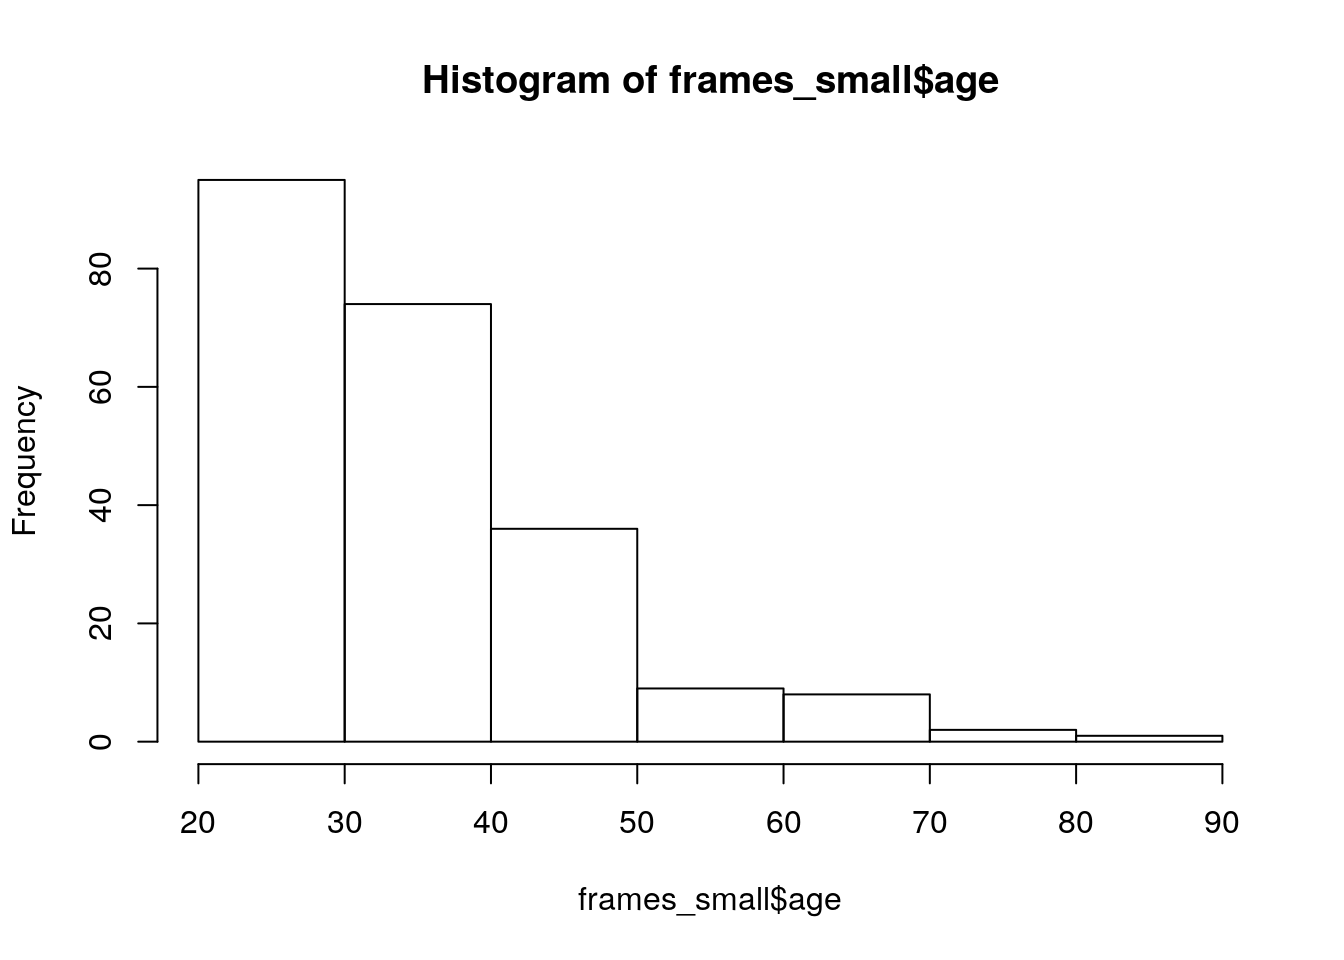
\includegraphics{2-01-visualisation_files/figure-latex/unnamed-chunk-2-1.pdf}
It's not exactly pretty -- though it's way nicer than the default plots that I remember seeing when I was younger -- but it gets the job done.

Okay, how do I create a histogram the tidyverse way? Much like base graphics, \textbf{ggplot2} recognises that histograms are such a fundamentally useful thing that there exists a ``geom'' (a term I'll explain in a moment) for them, but there's no way to draw a plot without going through a somewhat more convoluted process:

\begin{Shaded}
\begin{Highlighting}[]
\NormalTok{frames_small }\OperatorTok
\StringTok{  }\KeywordTok{ggplot}\NormalTok{(}\KeywordTok{aes}\NormalTok{(}\DataTypeTok{x =}\NormalTok{ age)) }\OperatorTok{+}
\StringTok{  }\KeywordTok{geom_histogram}\NormalTok{()}
\end{Highlighting}
\end{Shaded}

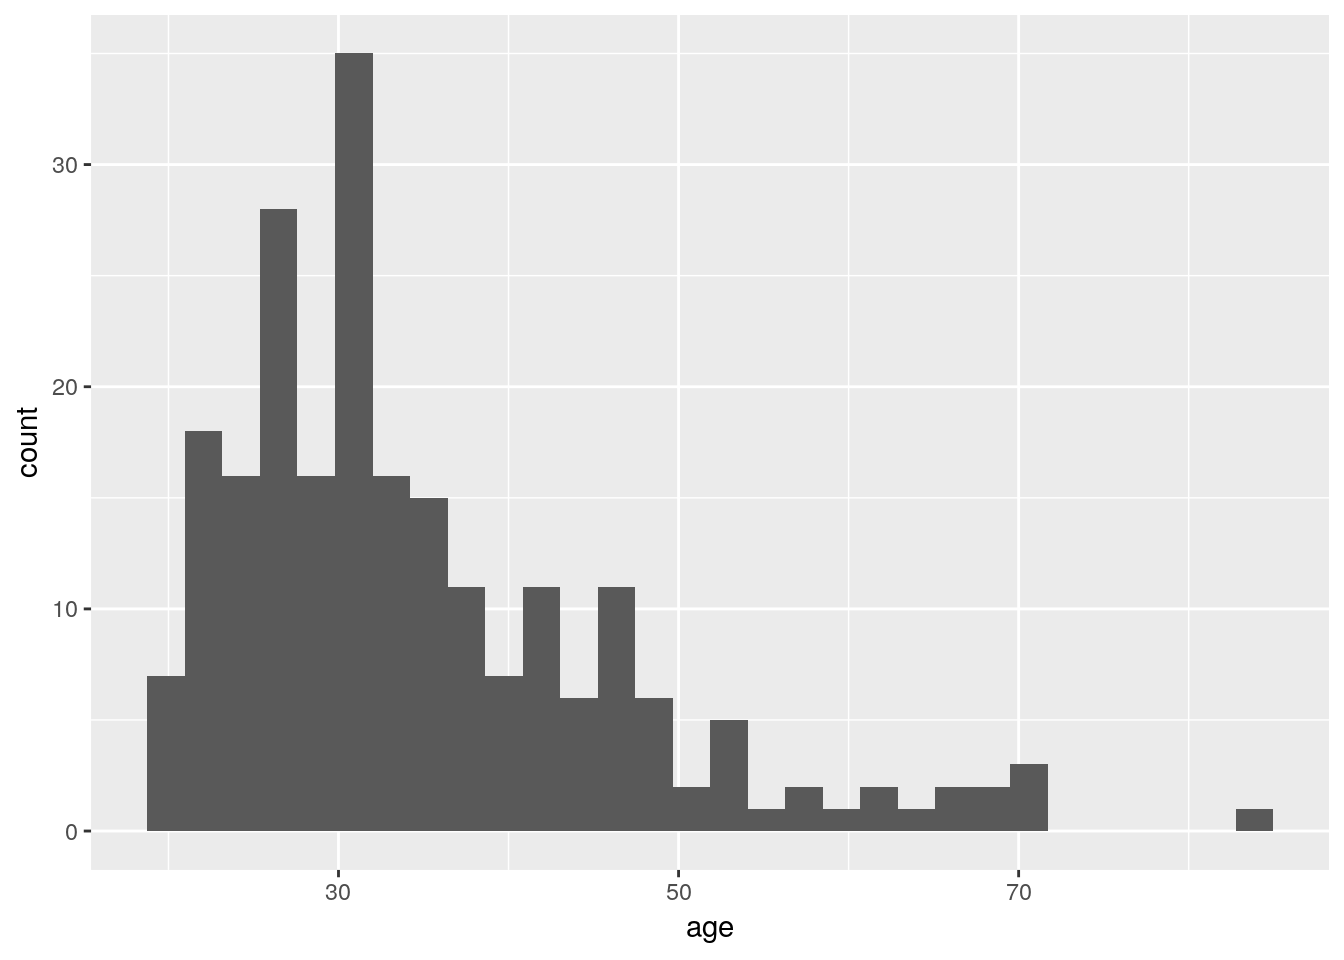
\includegraphics{2-01-visualisation_files/figure-latex/unnamed-chunk-3-1.pdf}
The output is prettier, admittedly, but our goal here wasn't to be pretty. Our goal was to be simple. For this comparison, the tidyverse approach is not as straightforward as base graphics.

Where the tidyverse versions shines is when we want to do something a little bit more complicated. Suppose I wanted two histograms side by side, plotting the age distribution separately by \texttt{condition}. In base graphics, it's a little cumbersome. What I have to do here is manually control the ``layout'' of the plot, dividing it into two separate panels and then drawing the histogram separately into each panel. That gives me code that looks like this:

\begin{Shaded}
\begin{Highlighting}[]
\KeywordTok{layout}\NormalTok{(}\KeywordTok{matrix}\NormalTok{(}\DecValTok{1}\OperatorTok{:}\DecValTok{2}\NormalTok{, }\DecValTok{1}\NormalTok{, }\DecValTok{2}\NormalTok{))}
\KeywordTok{hist}\NormalTok{(frames_small}\OperatorTok{$}\NormalTok{age[samplingframes}\OperatorTok{$}\NormalTok{condition }\OperatorTok{==}\StringTok{ "category"}\NormalTok{])}
\KeywordTok{hist}\NormalTok{(frames_small}\OperatorTok{$}\NormalTok{age[samplingframes}\OperatorTok{$}\NormalTok{condition }\OperatorTok{==}\StringTok{ "property"}\NormalTok{])}
\end{Highlighting}
\end{Shaded}

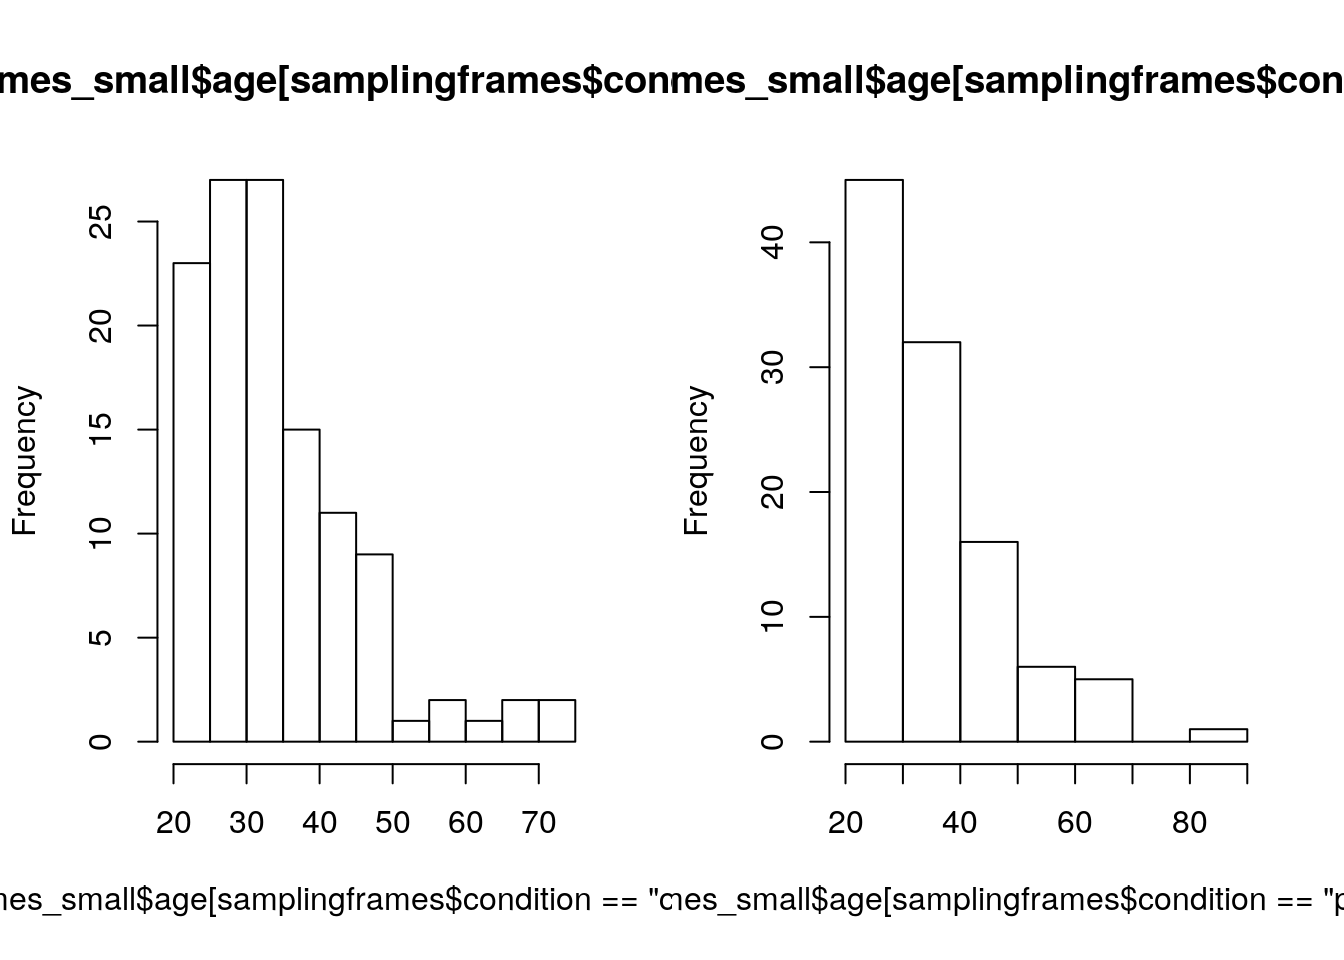
\includegraphics{2-01-visualisation_files/figure-latex/unnamed-chunk-4-1.pdf}

I need a lot more code as I did for the original version and I've ended up with an ugly plot. Of course, base graphics absolutely does allow me to do a better job than this, but I hope you can see that it will take quite a bit of effort to turn this into something readable.

What about the \textbf{ggplot2} version? It turns out that it's extremely easy. Splitting an existing plot into ``facets'' is a basic operation within \textbf{ggplot2} so all I need to do is add one line of code that specifies which variable to use to make the facets!
The result is actually kind of nice:

\begin{Shaded}
\begin{Highlighting}[]
\NormalTok{frames_small }\OperatorTok
\StringTok{  }\KeywordTok{ggplot}\NormalTok{(}\KeywordTok{aes}\NormalTok{(}\DataTypeTok{x =}\NormalTok{ age)) }\OperatorTok{+}
\StringTok{  }\KeywordTok{geom_histogram}\NormalTok{() }\OperatorTok{+}
\StringTok{  }\KeywordTok{facet_wrap}\NormalTok{(}\OperatorTok{~}\NormalTok{condition)}
\end{Highlighting}
\end{Shaded}

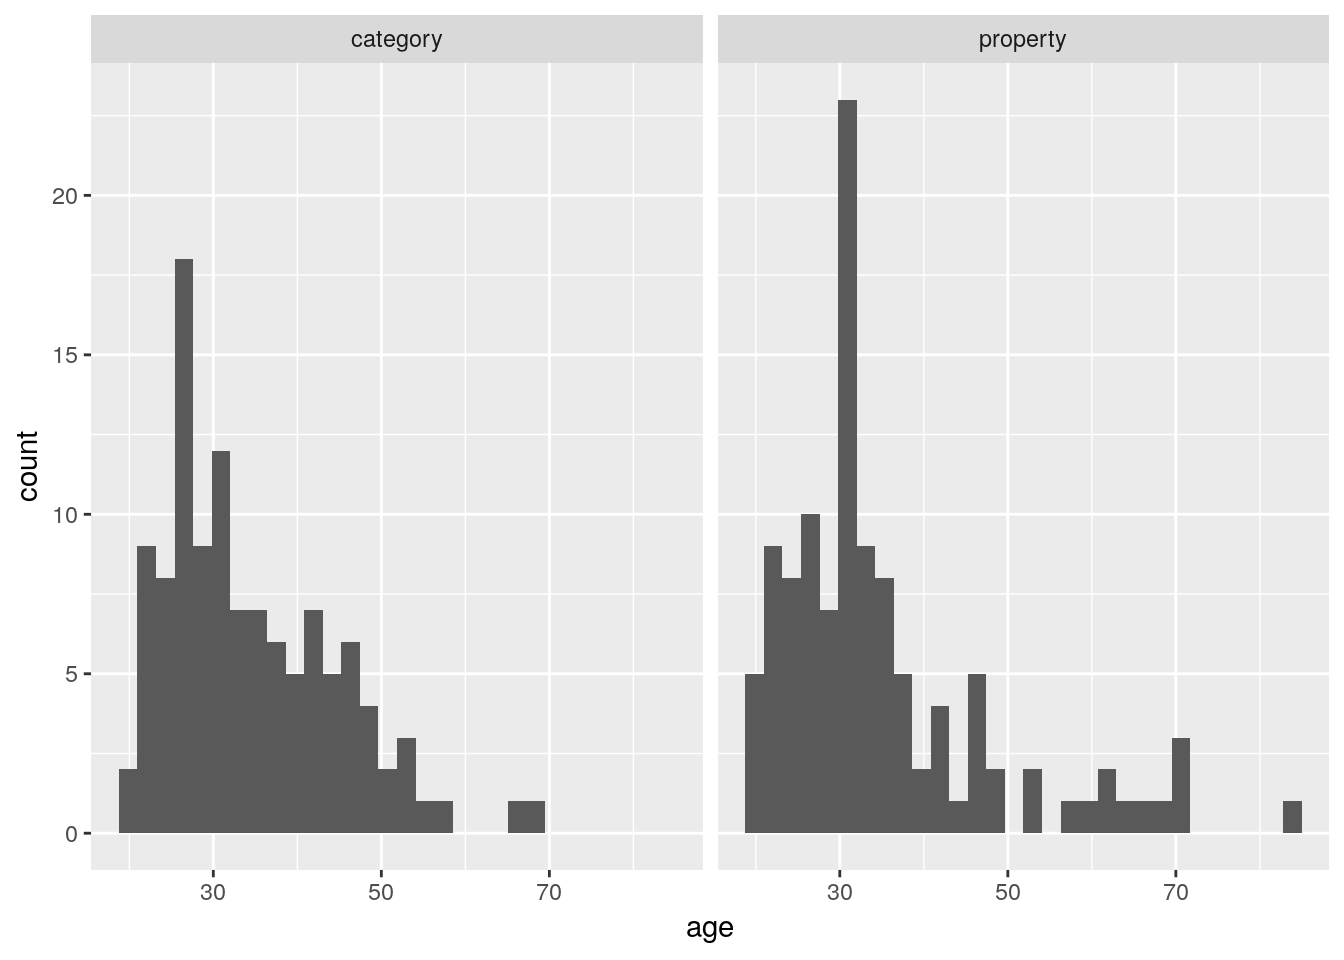
\includegraphics{2-01-visualisation_files/figure-latex/unnamed-chunk-5-1.pdf}

For me at least, this is the big advantage to the \textbf{ggplot2} approach. There's a certain amount of effort required to construct the basic plot, but once that is done, you can modify or manipulate that plot in an extremely flexible fashion with very little effort indeed. What I've found in practice is that the low-effort to making changes makes me much more willing to ``play around'' with different ways of visualising the data. So, while I'll admit that there are some situations where I resort to using base graphics (mostly when I have a very unconventional graph to draw), I tend to find the tidyverse approach works better in the majority of cases.

As far as what the data visualisation is telling us: the distribution of ages was mostly in the 20-40 age range with a modest positive skew. That's pretty typical of these studies. More importantly, it's pretty clear from inspection that there's not much of a difference in the age distribition across conditions, which is what I'd hope to see given that people were assigned randomly.

\hypertarget{scatter-plot}{%
\section{Scatter plot}\label{scatter-plot}}

The second kind of plot I'll talk about is a scatter plot, in which each observation is drawn as a point, and the graph shows the values on one variable against the values on another. It's such a simply plot that I'll use it as a mechanism to illustrate the key ideas in \textbf{ggplot2}.

Lets build our plot piece by piece. The data we want to use here come from \texttt{frames\_small}, so the first thing we'll do is pipe this data set to the \texttt{ggplot()} function and see what it produces:

\begin{Shaded}
\begin{Highlighting}[]
\NormalTok{frames_small }\OperatorTok\StringTok{ }
\StringTok{  }\KeywordTok{ggplot}\NormalTok{()}
\end{Highlighting}
\end{Shaded}


\includegraphics{2-01-visualisation_files/figure-latex/unnamed-chunk-6-1.pdf}

In retrospect that's unsurprising. Although we've passed the data to \texttt{ggplot()}, we haven't told R what it ought to \emph{do} with these data, so the output is simply a blank canvas! To make some progress, the next step is to specify a \texttt{mapping} for the plot that will tell R something about what roles the different variables play. In \textbf{ggplot2} these mappings are described as a set of ``\emph{aesthetics}'', defined using the \texttt{aes()} function. There are many different aesthetics that can be used, but for a scatter plot the only things we really \emph{need} to specify as aesthetics are the variable on the \texttt{x} axis and the variable on the \texttt{y} axis. So if we wanted to plot \texttt{y\ =\ response} against \texttt{x\ =\ age}, this is the mapping we would need:

\begin{Shaded}
\begin{Highlighting}[]
\NormalTok{frames_small }\OperatorTok\StringTok{ }
\StringTok{  }\KeywordTok{ggplot}\NormalTok{(}\DataTypeTok{mapping =} \KeywordTok{aes}\NormalTok{(}\DataTypeTok{x =}\NormalTok{ age, }\DataTypeTok{y =}\NormalTok{ response))}
\end{Highlighting}
\end{Shaded}

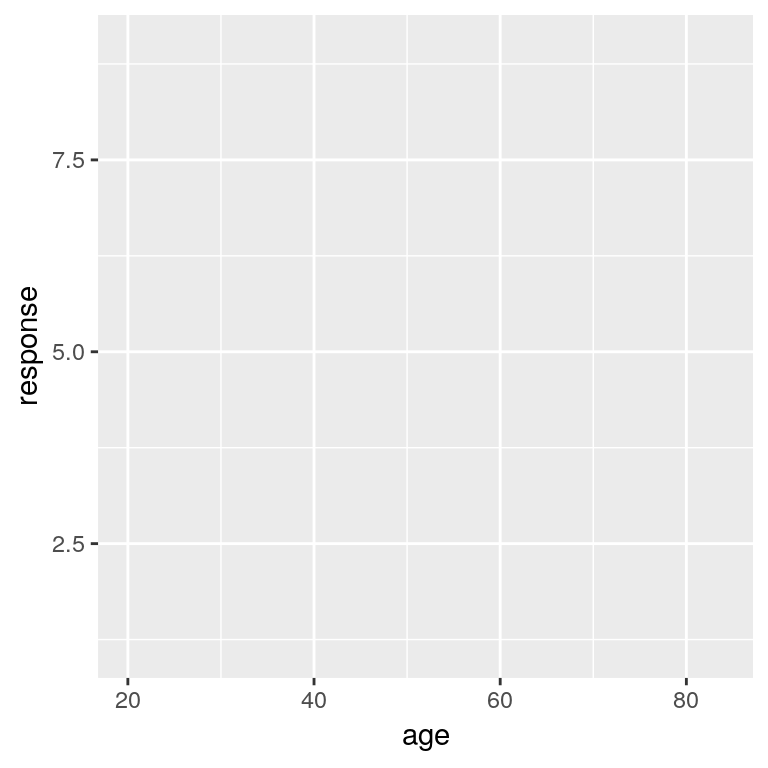
\includegraphics{2-01-visualisation_files/figure-latex/unnamed-chunk-7-1.pdf}

Hm. That's clearly some progress. The canvas now has the axis labels and gridlines reflecting the fact that R now knows which variables we're hoping to ploy. However, we still don't have any data, because we haven't told R what it should \emph{do} to render the data. This is the role played by \emph{geoms}, which specify different ways in which data can be displayed. Since we're trying to draw a scatter plot, I'm going to use the simplest possible \emph{geom} function, namely \texttt{geom\_point()}. All it does is draw a dot for each data point:

\begin{Shaded}
\begin{Highlighting}[]
\NormalTok{frames_small }\OperatorTok\StringTok{ }
\StringTok{  }\KeywordTok{ggplot}\NormalTok{(}\DataTypeTok{mapping =} \KeywordTok{aes}\NormalTok{(}\DataTypeTok{x =}\NormalTok{ age, }\DataTypeTok{y =}\NormalTok{ response)) }\OperatorTok{+}
\StringTok{  }\KeywordTok{geom_point}\NormalTok{()}
\end{Highlighting}
\end{Shaded}

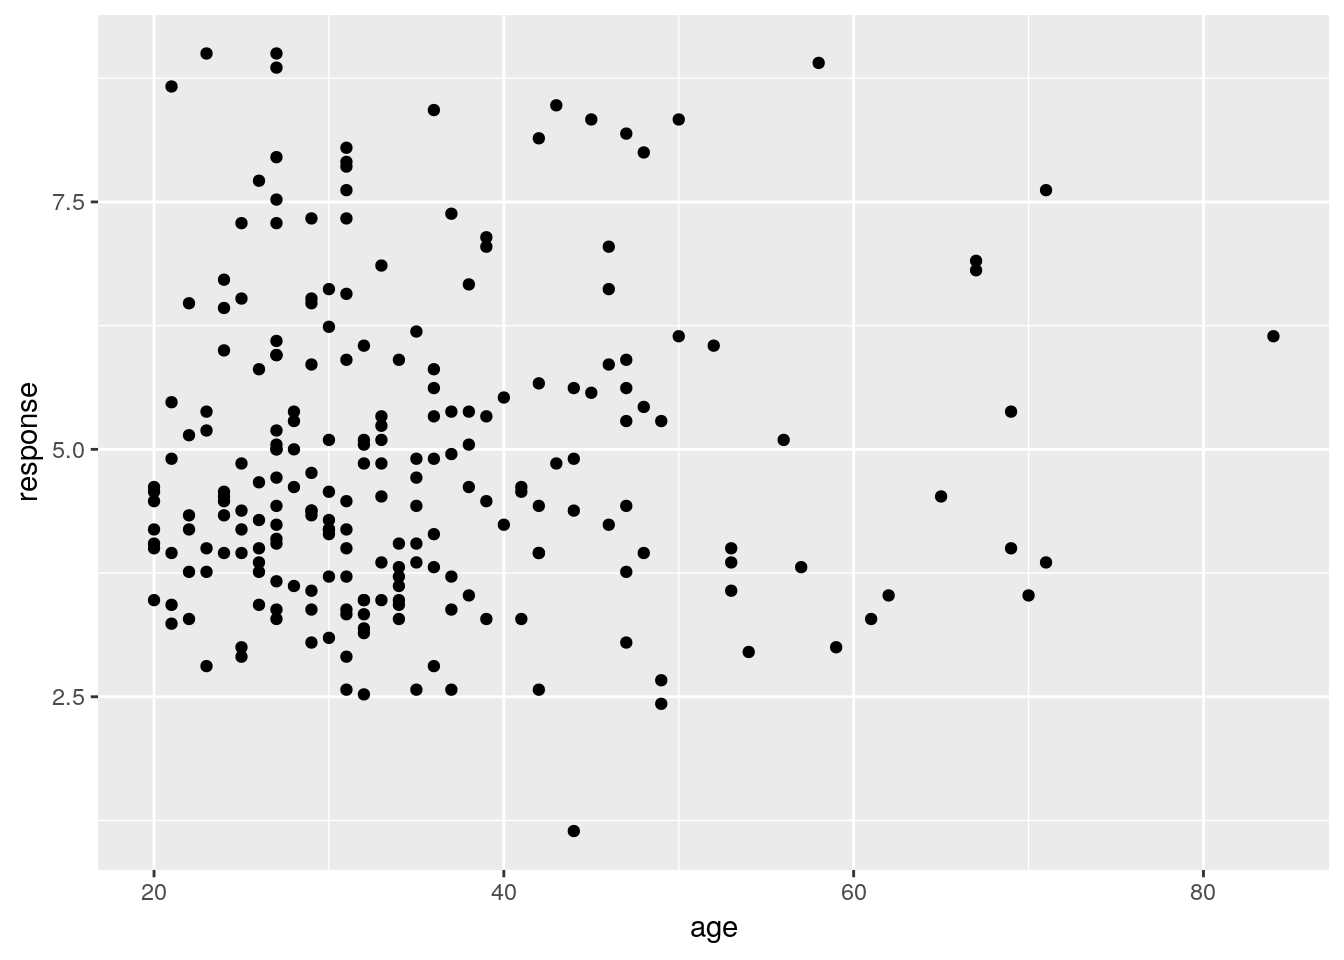
\includegraphics{2-01-visualisation_files/figure-latex/unnamed-chunk-8-1.pdf}

Now we have our scatter plot! From visual inspection there doesn't seem to be any strong relationship between the \texttt{age} of a participant and the \texttt{response} they give. Again, that's not surprising, but useful to check.

It's worth highlighting the different roles played by aesthetics and geoms. For instance, I could have expanded the list of aesthetics to include \texttt{colour\ =\ condition}, which would indicate that the colour of each dot should indicated which condition the participant in question was assigned to:

\begin{Shaded}
\begin{Highlighting}[]
\NormalTok{frames_small }\OperatorTok\StringTok{ }
\StringTok{  }\KeywordTok{ggplot}\NormalTok{(}\DataTypeTok{mapping =} \KeywordTok{aes}\NormalTok{(}\DataTypeTok{x =}\NormalTok{ age, }\DataTypeTok{y =}\NormalTok{ response, }\DataTypeTok{colour =}\NormalTok{ condition)) }\OperatorTok{+}
\StringTok{  }\KeywordTok{geom_point}\NormalTok{()}
\end{Highlighting}
\end{Shaded}

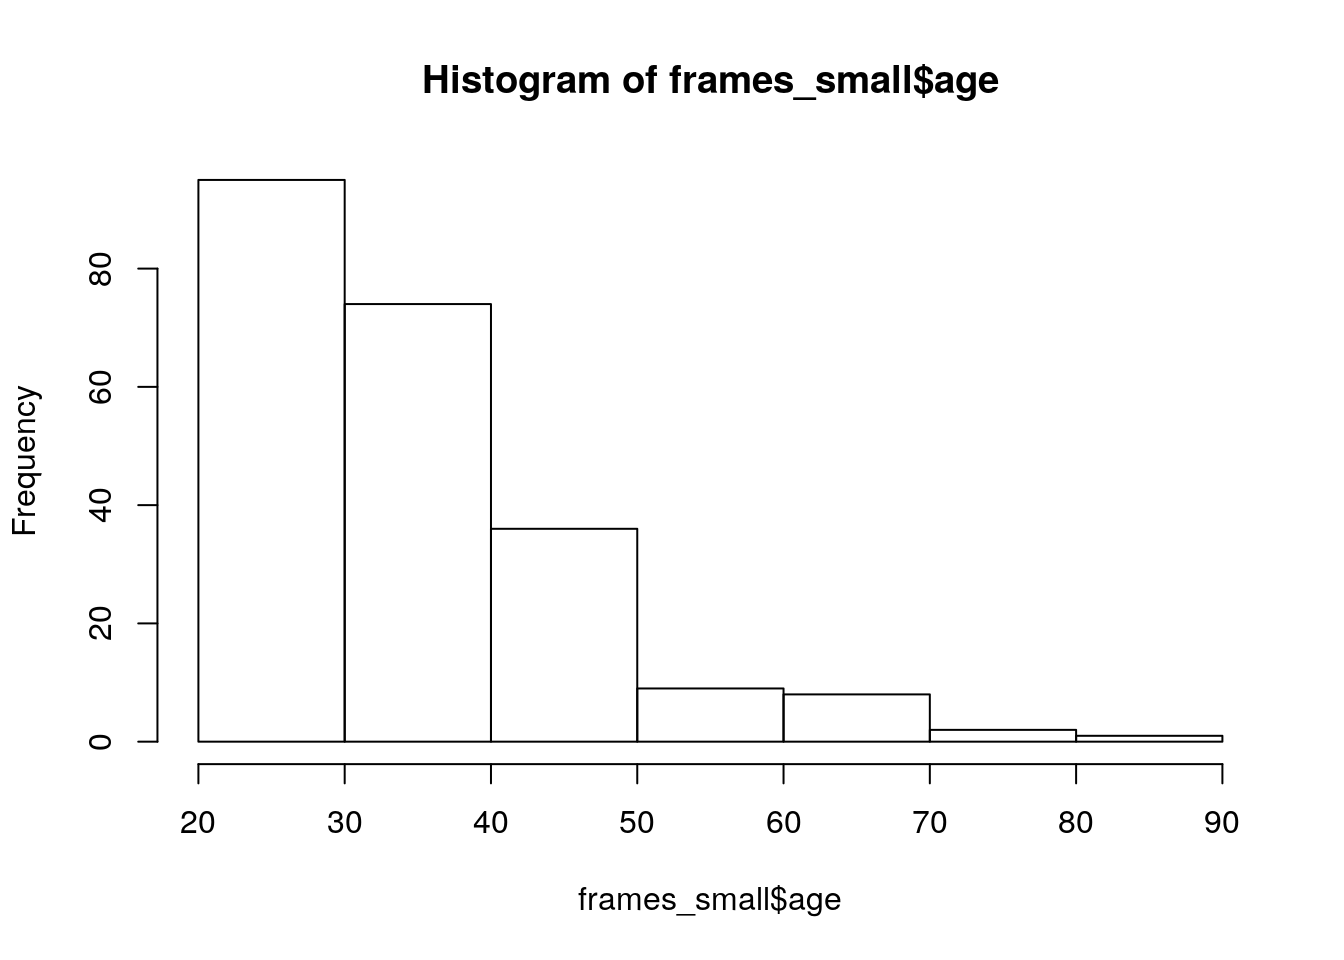
\includegraphics{2-01-visualisation_files/figure-latex/unnamed-chunk-9-1.pdf}

However, I can also add new geoms that will draw new layers to the plot. For example, \texttt{geom\_rug} adds a visual representation of the marginal distribution of the data on both axes, like this:

\begin{Shaded}
\begin{Highlighting}[]
\NormalTok{frames_small }\OperatorTok\StringTok{ }
\StringTok{  }\KeywordTok{ggplot}\NormalTok{(}\DataTypeTok{mapping =} \KeywordTok{aes}\NormalTok{(}\DataTypeTok{x =}\NormalTok{ age, }\DataTypeTok{y =}\NormalTok{ response, }\DataTypeTok{colour =}\NormalTok{ condition)) }\OperatorTok{+}
\StringTok{  }\KeywordTok{geom_point}\NormalTok{() }\OperatorTok{+}\StringTok{ }
\StringTok{  }\KeywordTok{geom_rug}\NormalTok{()}
\end{Highlighting}
\end{Shaded}

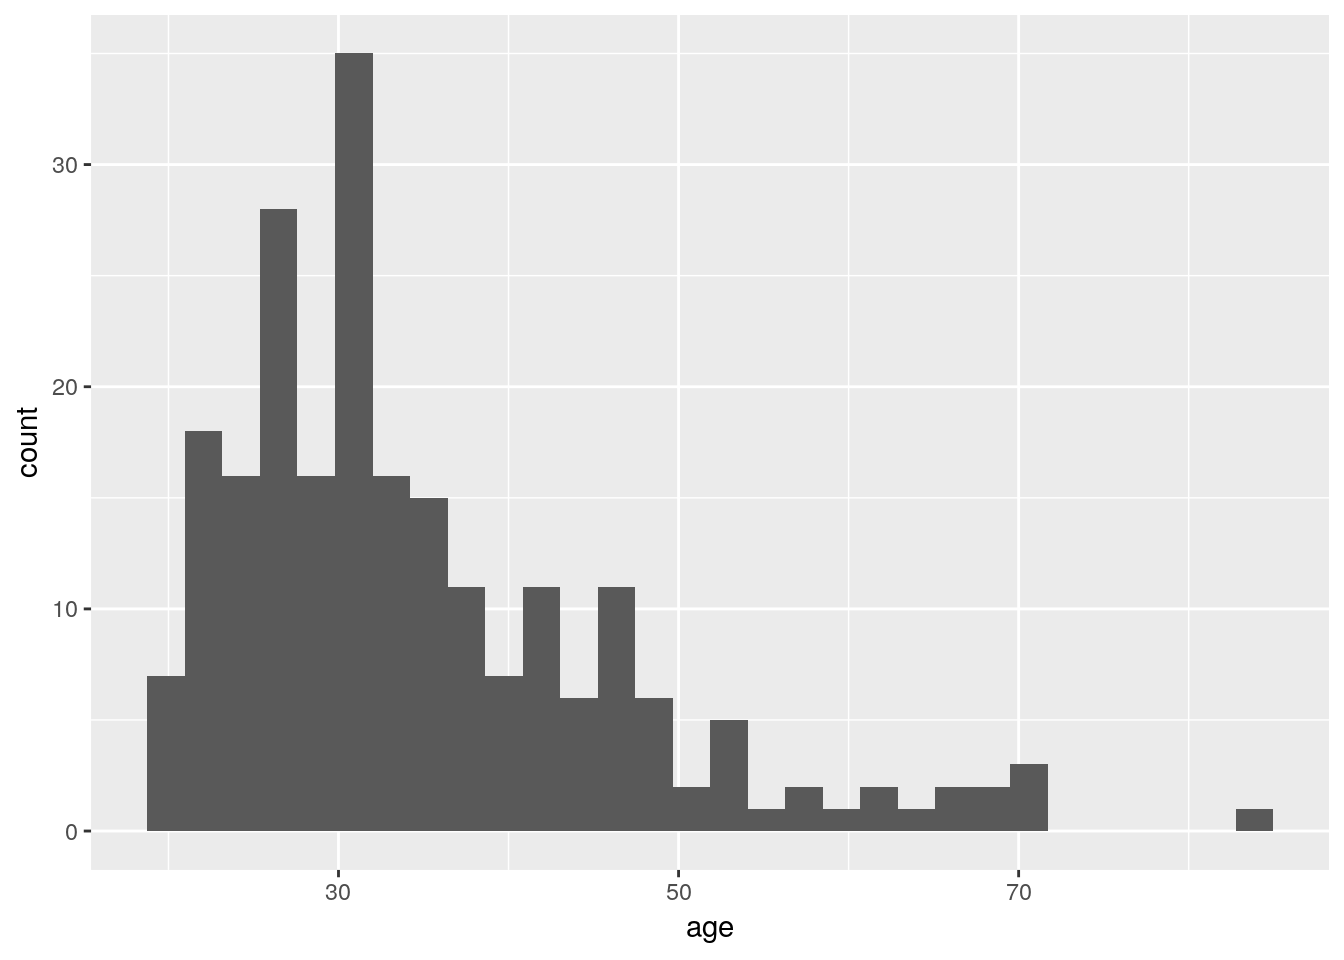
\includegraphics{2-01-visualisation_files/figure-latex/unnamed-chunk-10-1.pdf}

Notice the style here. A pretty typical way to build a visualisation is to construct it in layers, \emph{adding} new geoms, aesthetics and other plot customisations as you go. So you'll often end up with code structured like this:\footnote{There is a little bit of weirdness to this. Once you've gotten accustomed to using the pipe operator \texttt{\%\textgreater{}\%} it starts to feel like we should be writing code like \texttt{data\ \%\textgreater{}\%\ ggplot()\ \%\textgreater{}\%\ geom()\ \%\textgreater{}\%\ etc} rather than \texttt{data\ \%\textgreater{}\%\ (ggplot()\ +\ geom()\ +\ etc)}. This is purely for historical reasons: \textbf{ggplot2} predates the pipe operator and so unlike everything else in \textbf{tidyverse} it's not very compatible with \texttt{\%\textgreater{}\%}.}

\begin{verbatim}
DATA %>%
  ggplot(aes( LIST_OF_AESTHETICS )) +
  A_GEOM +
  ANOTHER_GEOM +
  ETC
\end{verbatim}

In any case, looking at these scatter plots there's nothing that immediately suggests and differential patterns of responding as a function of age but there is a hint that responses are lower in the property sampling condition (blue) than in the category sampling condition (red).

\hypertarget{bar-graphs}{%
\section{Bar graphs}\label{bar-graphs}}

The humble bar graph is a staple in the scientific literature, and can be rendered by \textbf{ggplot2} with the assistance of the \texttt{geom\_bar()} function. Suppose I want to check that the gender distribution for this study was relatively even across conditions.\footnote{In this study I asked people to respond with a three value questionnaire, with options for ``male'', ``female'' and ``other'' as possible gender identities. I'm not entirely satisfied with this as a measurement method though, and the question wasn't compulsory to answer.} To do that, I'll set up my mapping with \texttt{gender} on the x-axis (using \texttt{ggplot} to initialise the plot and \texttt{aes} to specify the aesthetics), create separate panels for each \texttt{condition} (using \texttt{facet\_wrap} which I'll explain in more detail below), and then use \texttt{geom\_bar()} to draw the plot:

\begin{Shaded}
\begin{Highlighting}[]
\NormalTok{frames_small }\OperatorTok
\StringTok{  }\KeywordTok{ggplot}\NormalTok{(}\KeywordTok{aes}\NormalTok{(}\DataTypeTok{x =}\NormalTok{ gender)) }\OperatorTok{+}\StringTok{  }\CommentTok{# set up the mapping}
\StringTok{  }\KeywordTok{facet_wrap}\NormalTok{(}\OperatorTok{~}\NormalTok{condition) }\OperatorTok{+}\StringTok{   }\CommentTok{# split it into plots}
\StringTok{  }\KeywordTok{geom_bar}\NormalTok{()                 }\CommentTok{# add the bars!}
\end{Highlighting}
\end{Shaded}

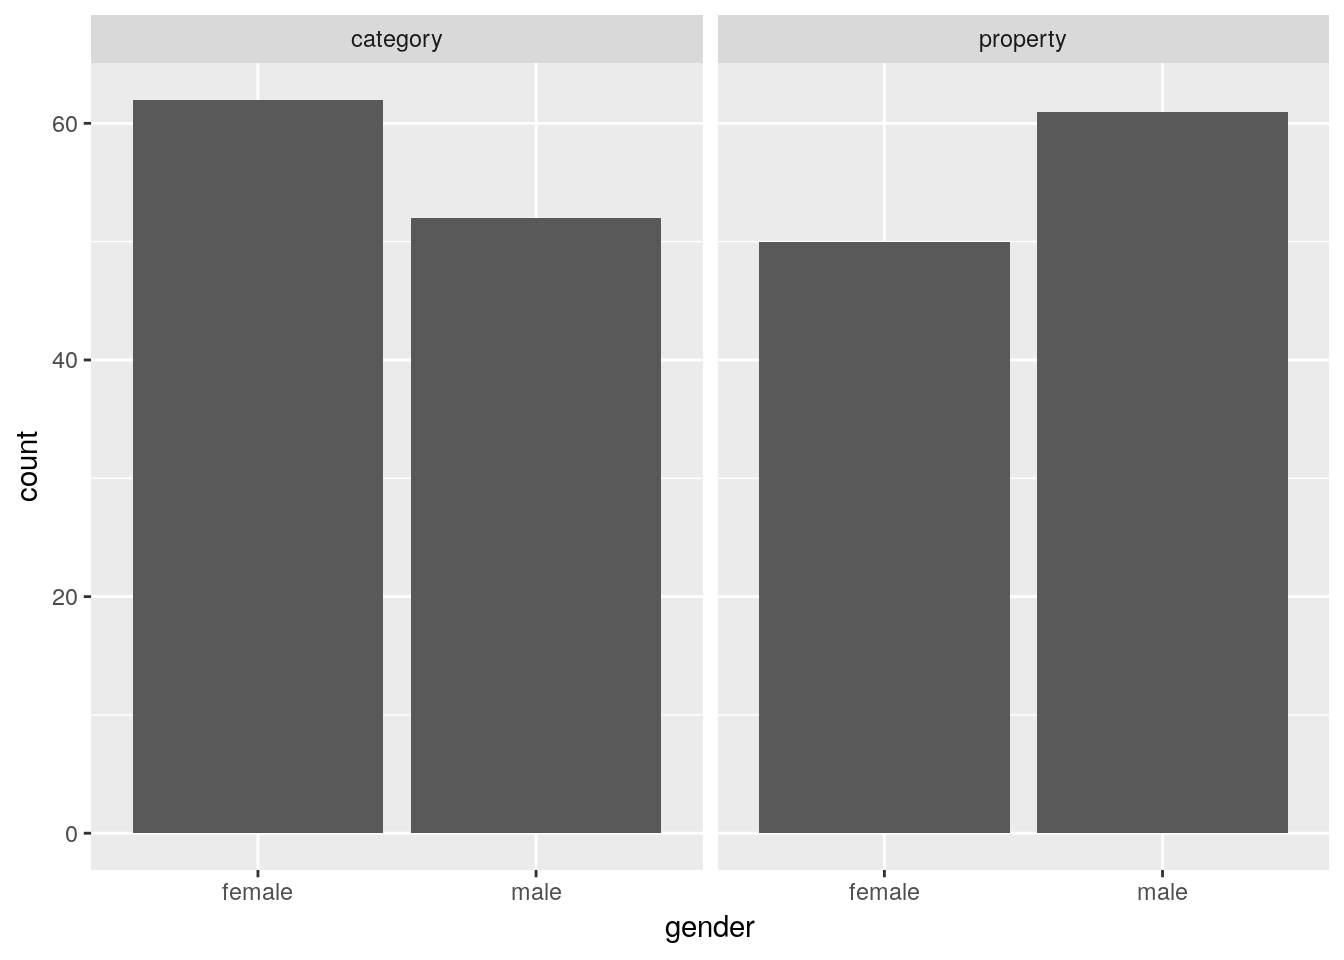
\includegraphics{2-01-visualisation_files/figure-latex/unnamed-chunk-11-1.pdf}

As one would expect for random assignment there's a little unevenness but not very much. That looks totally fine to me, and at this point I've convinced myself that the \texttt{age} and \texttt{gender} variables really don't matter very much, so I can start digging into the details about how the manipulated variables of theoretical interest (\texttt{sample\_size}, \texttt{condition} and \texttt{test\_loc}) relate to the inductive generalisation \texttt{response} judgment that people make\ldots{}

\hypertarget{box-plots}{%
\section{Box plots}\label{box-plots}}

Another classic data visualisation used in psychology is the box plot (due to John Tukey), which presents a schematic representation of the distribution of responses. Box plots can be drawn in many different forms, but the most conventional version the median value (50th percentile) as a thick horizontal line, contained within a box that spans the range from 25th percentile to the 75th percentile. Above and below the box are the ``whiskers'' which extend to cover the full range of the data (after excluding outliers).
Outliers are plotted as individual dots. Note that in this context an outlier is conventionally defined as a point that lies more than 1.5 times the interquartile range from the median: this is often a convenient heuristic to use but it's not magical. Don't read too much into the fact that a data set includes outliers!

To construct a boxplot using \textbf{ggplot2} all we need to do is add a \texttt{geom\_boxplot()} to the graph. So if I want to plot the distribution of \texttt{response} values across participants (averaged across test items) separately for each \texttt{condition}, I could do this:

\begin{Shaded}
\begin{Highlighting}[]
\NormalTok{frames_small }\OperatorTok
\StringTok{  }\KeywordTok{ggplot}\NormalTok{(}\KeywordTok{aes}\NormalTok{(}\DataTypeTok{x =}\NormalTok{ condition, }\DataTypeTok{y =}\NormalTok{ response)) }\OperatorTok{+}\StringTok{ }
\StringTok{  }\KeywordTok{geom_boxplot}\NormalTok{()}
\end{Highlighting}
\end{Shaded}

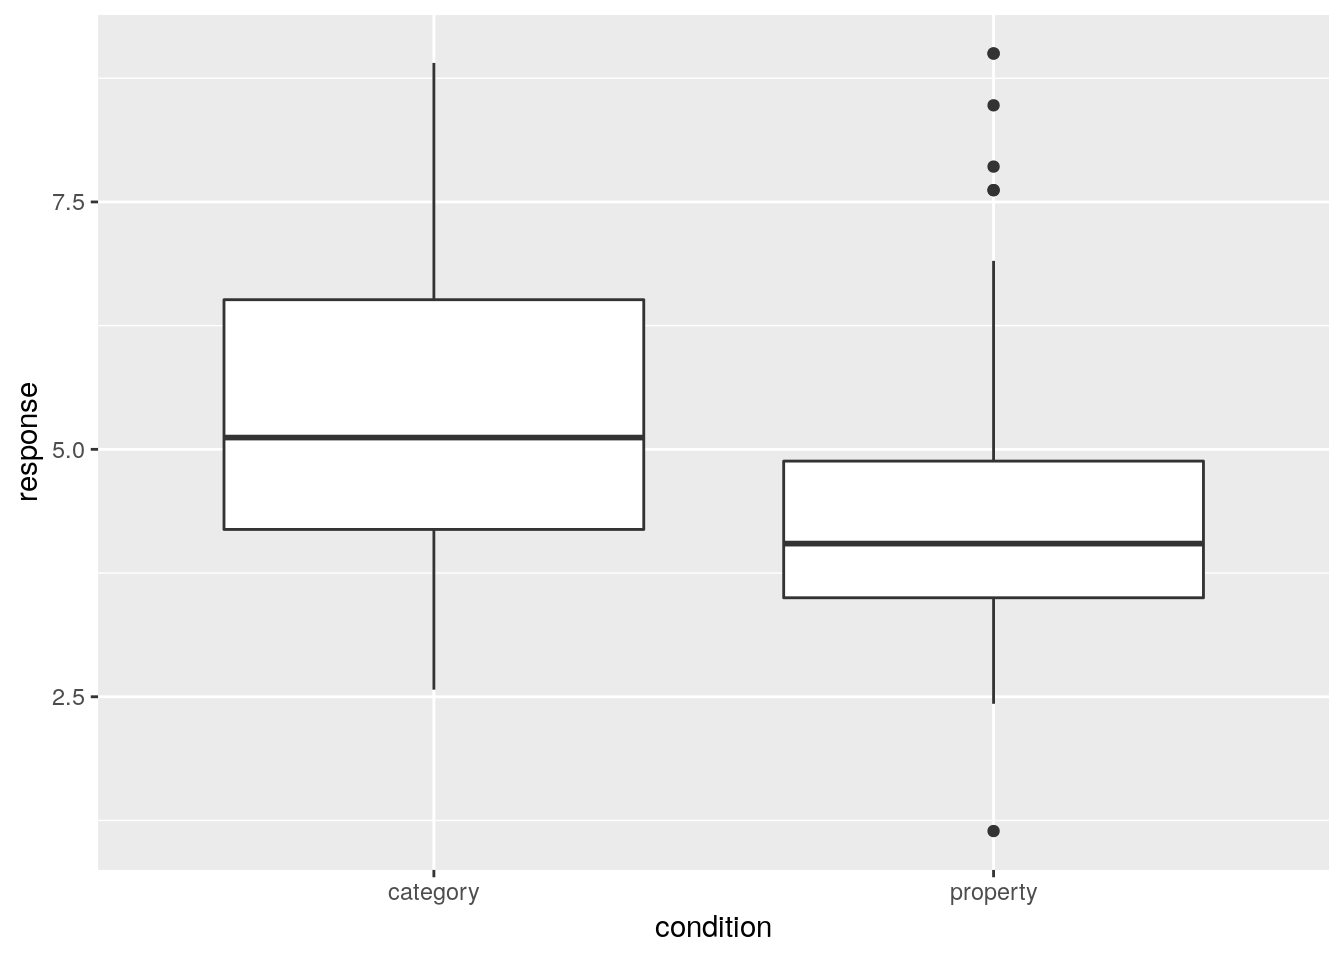
\includegraphics{2-01-visualisation_files/figure-latex/unnamed-chunk-12-1.pdf}

This plot is easy to interpret and provides our first hint that there is in fact something of interest going on in these data. On a first pass, it rather looks like people are less willing to make inductive generalisations (i.e., give lower scores) in the property sampling condition than in the category sampling condition!

\hypertarget{violin-plots}{%
\section{Violin plots}\label{violin-plots}}

Although the box plot is an old method for visualising the key characteristics of distribution it's a very good one. It's visually simple, meaning that you can put a lot of box plots in a single graph without causing too much clutter, yet it still conveys a lot of information about the distribution. So there are many situations in which they are worth including (we'll see a good example in a moment)

On the other hand, for the specific situation here where there are only two disributions to be displayed, it does seem like we could do better. With the state of computing having advanced quite dramatically over recent decades, it is extremely easy to construct more complicated \emph{kernel density estimates} of the shape of the population from which the sample is drawn. The \emph{violin plot} provides a method for visually displaying a kernel density estimate. If we switch from \texttt{geom\_boxplot()} to \texttt{geom\_violin()} the resulting plot looks like this:

\begin{Shaded}
\begin{Highlighting}[]
\NormalTok{frames_small }\OperatorTok
\StringTok{  }\KeywordTok{ggplot}\NormalTok{(}\KeywordTok{aes}\NormalTok{(}\DataTypeTok{x =}\NormalTok{ condition, }\DataTypeTok{y =}\NormalTok{ response)) }\OperatorTok{+}\StringTok{ }
\StringTok{  }\KeywordTok{geom_violin}\NormalTok{()}
\end{Highlighting}
\end{Shaded}


\includegraphics{2-01-visualisation_files/figure-latex/unnamed-chunk-13-1.pdf}

It's intuitively obvious what this plot is doing: the ``width'' of the violin\footnote{Yeah, they never actually look like violins. We should just give up and call them blob plots} at each point shows the estimated ``density'' of the population distribution at that point. To make it a little clearer what this is showing, let's overlay the raw data on the plot, using the \texttt{geom\_jitter()} method to make it a little easier to see:

\begin{Shaded}
\begin{Highlighting}[]
\NormalTok{frames_small }\OperatorTok
\StringTok{  }\KeywordTok{ggplot}\NormalTok{(}\KeywordTok{aes}\NormalTok{(}\DataTypeTok{x =}\NormalTok{ condition, }\DataTypeTok{y =}\NormalTok{ response)) }\OperatorTok{+}\StringTok{ }
\StringTok{  }\KeywordTok{geom_violin}\NormalTok{() }\OperatorTok{+}
\StringTok{  }\KeywordTok{geom_jitter}\NormalTok{()}
\end{Highlighting}
\end{Shaded}

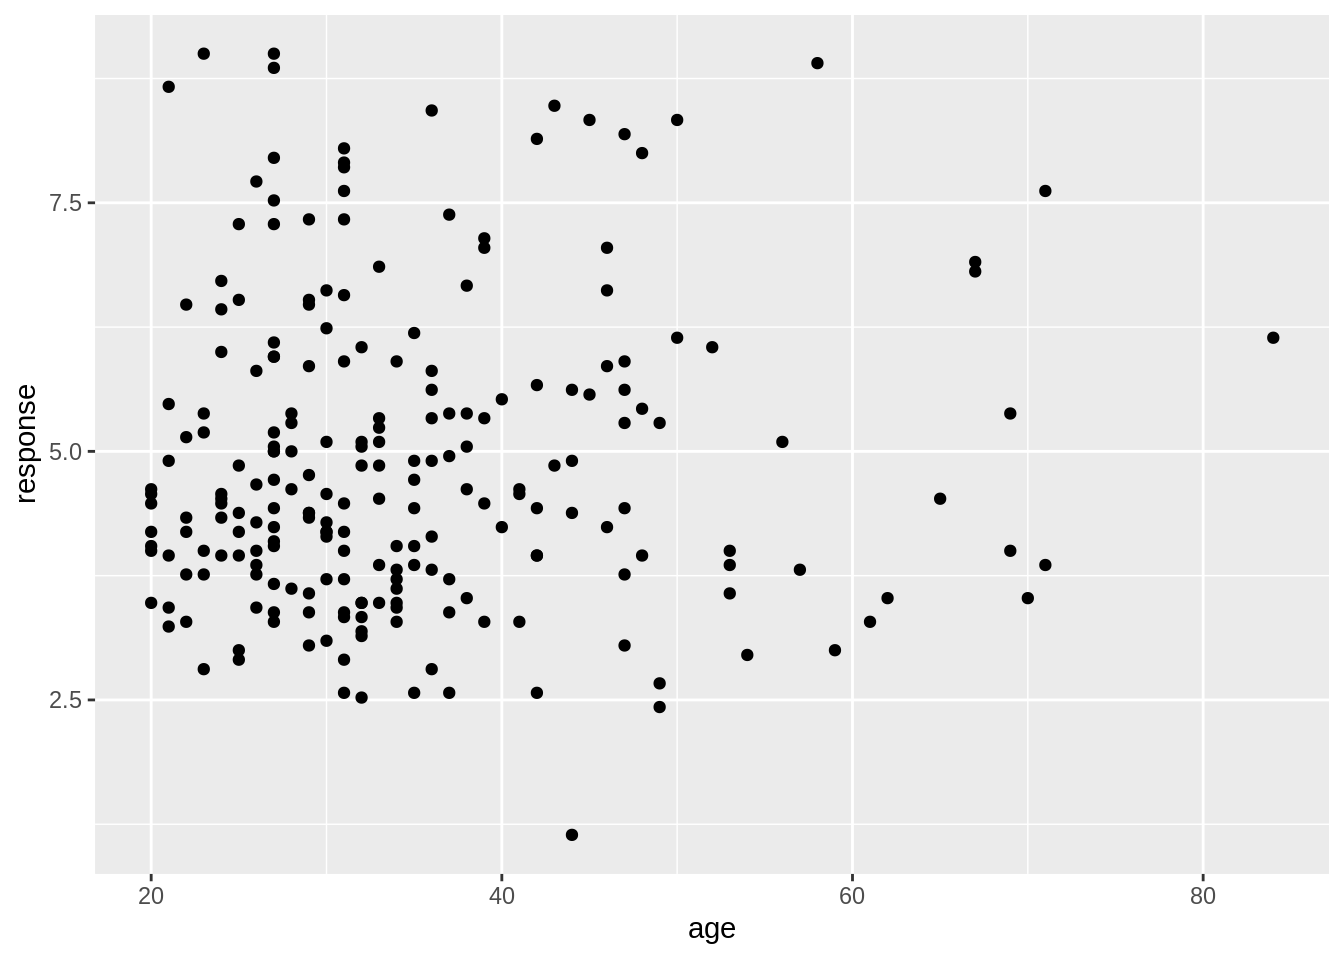
\includegraphics{2-01-visualisation_files/figure-latex/unnamed-chunk-14-1.pdf}

As you can see, in the property sampling condition the data are concentrated pretty tightly around 4.5, whereas in the category sampling condition the data are shifted upwards and spread out. That's what produces the different shapes in the violin plots.

\hypertarget{facetted-plots}{%
\section{Facetted plots}\label{facetted-plots}}

The big problem I have with the data visualisations we've drawn so far is that we're really not getting a very fine grained story. When we constructed the \texttt{response} variable for the \texttt{frames\_small} data frame we averaged over all three values of \texttt{sample\_size} and across all seven values of \texttt{test\_loc}. That's fine as a first pass if we want to take a quick look at the difference across \texttt{condition}, but in real world data analysis we need to hold ourselves to higher standards! So lets go back to the raw \texttt{frames} data, and see if we can find a better visualisation. This brings us naturally to the topic of \emph{faceting} a plot\ldots{}

A common task in data visualisation is to construct facet plots that display an existing plot separately for each group. We've seen this twice already, once in the histogram at the start of this section and previously in the \href{./prelude-to-data.html}{prelude}. In both cases I used \texttt{facet\_wrap()} to do the work, using the \texttt{\textasciitilde{}} operator to specify a one-sided formula (e.g., \texttt{\textasciitilde{}condition}). This function splits the plot by the levels of a factor, and then ``wraps'' them around to keep the plot tidy. For example, if there were 16 levels of the \texttt{condition} variable then \texttt{facet\_wrap()} would probably give us a 4x4 grid.

If you want more precise control over the faceting, an alternative approach is to use \texttt{facet\_grid()}. For instance, let's suppose I want to draw separate boxplots for the \texttt{response} variable for every possible \texttt{test\_item}, broken down by \texttt{condition} and \texttt{sample\_size}. That's going to give us 42 boxplots, so some degree of care is required here! Here's my first attempt:

\begin{Shaded}
\begin{Highlighting}[]
\NormalTok{samplingframes }\OperatorTok\StringTok{                               }\CommentTok{# start with the full data set!}
\StringTok{  }\KeywordTok{ggplot}\NormalTok{(}\KeywordTok{aes}\NormalTok{(}
    \DataTypeTok{x =} \KeywordTok{factor}\NormalTok{(test_item),               }\CommentTok{# treat "test_item" as categorical}
    \DataTypeTok{y =}\NormalTok{ response)) }\OperatorTok{+}\StringTok{                     }\CommentTok{# y variable is "response"}
\StringTok{  }\KeywordTok{facet_grid}\NormalTok{(sample_size }\OperatorTok{~}\StringTok{ }\NormalTok{condition) }\OperatorTok{+}\StringTok{  }\CommentTok{# add faceting}
\StringTok{  }\KeywordTok{geom_boxplot}\NormalTok{()                         }\CommentTok{# oh, right... add the boxplots :-)}
\end{Highlighting}
\end{Shaded}

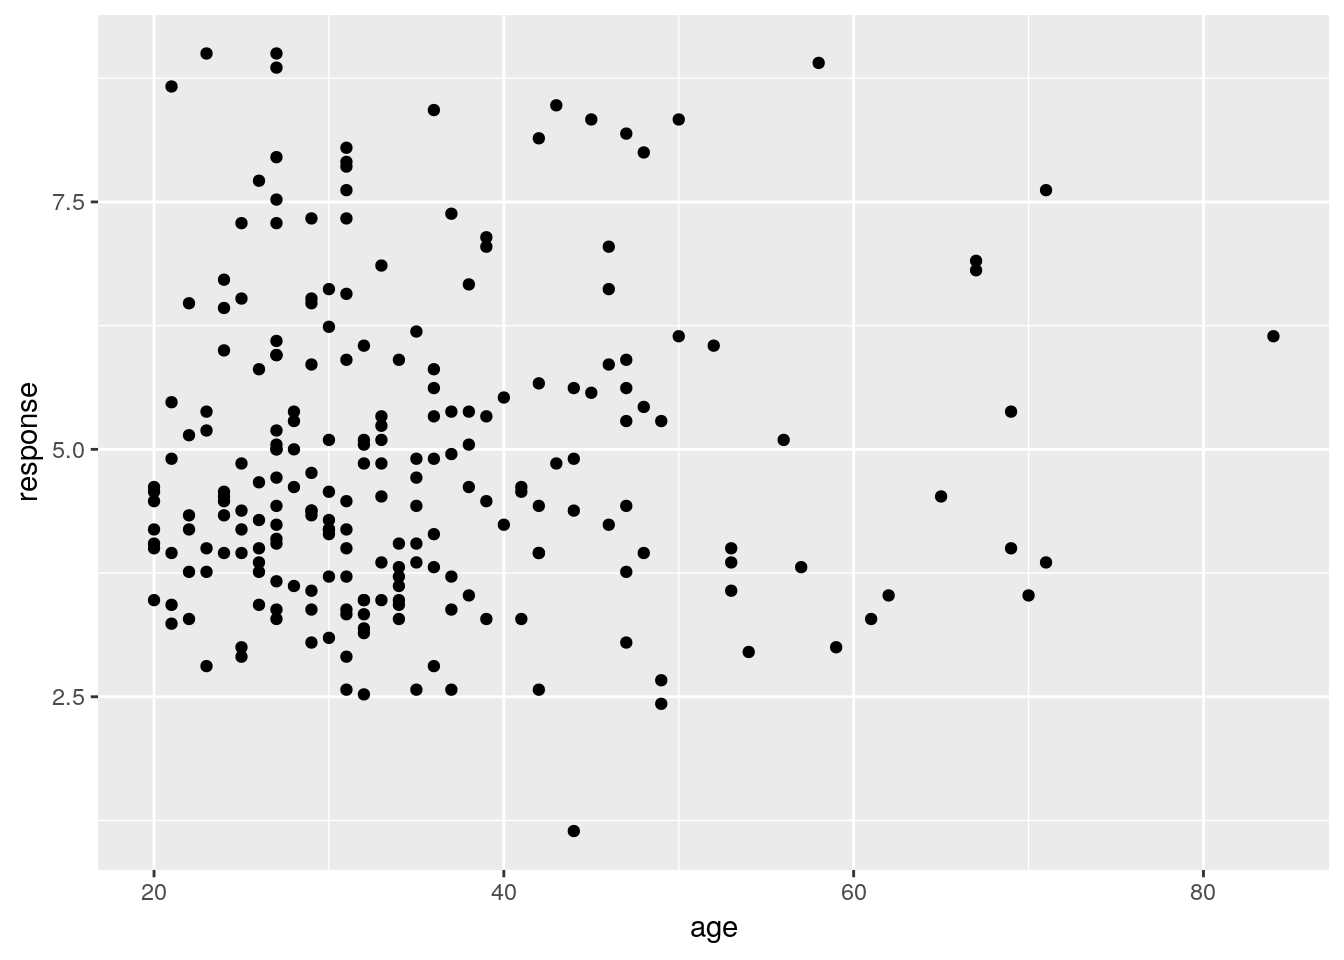
\includegraphics{2-01-visualisation_files/figure-latex/unnamed-chunk-15-1.pdf}

That's not bad as a first pass. There's a few things I'd like to do to tidy it though:

\begin{itemize}
\tightlist
\item
  Flip the grid by changing the formula to \texttt{condition\ \textasciitilde{}\ sample\_size}
\item
  Reorder the sample size facets by changing \texttt{sample\_size} to a factor
\item
  Adding nicer axis labels using \texttt{xlab()} and \texttt{ylab()}
\item
  Make the ``outliers'' less obtrusive using transparency
\end{itemize}

To do this, the first thing I'm going to do is use \texttt{dplyr::mutate} -- discussed in the previous section -- to convert the \texttt{sample\_size} variable to a factor, and make sure the levels are specified in the order I want them to appear in the plot:

\begin{Shaded}
\begin{Highlighting}[]
\NormalTok{samplingframes <-}\StringTok{ }\NormalTok{samplingframes }\OperatorTok
\StringTok{  }\KeywordTok{mutate}\NormalTok{(}\DataTypeTok{sample_size =} \KeywordTok{factor}\NormalTok{(sample_size, }\DataTypeTok{levels =} \KeywordTok{c}\NormalTok{(}\StringTok{"small"}\NormalTok{,}\StringTok{"medium"}\NormalTok{,}\StringTok{"large"}\NormalTok{)))}
\end{Highlighting}
\end{Shaded}

Now my command to draw the plot looks like this:

\begin{Shaded}
\begin{Highlighting}[]
\NormalTok{samplingframes }\OperatorTok\StringTok{                               }
\StringTok{  }\KeywordTok{ggplot}\NormalTok{(}\KeywordTok{aes}\NormalTok{(}
    \DataTypeTok{x =} \KeywordTok{factor}\NormalTok{(test_item),               }
    \DataTypeTok{y =}\NormalTok{ response)) }\OperatorTok{+}\StringTok{                     }
\StringTok{  }\KeywordTok{facet_grid}\NormalTok{(condition }\OperatorTok{~}\StringTok{ }\NormalTok{sample_size) }\OperatorTok{+}\StringTok{  }\CommentTok{# reversed faceting}
\StringTok{  }\KeywordTok{geom_boxplot}\NormalTok{(}\DataTypeTok{outlier.alpha =} \FloatTok{0.1}\NormalTok{) }\OperatorTok{+}\StringTok{    }\CommentTok{# alpha sets the transparency}
\StringTok{  }\KeywordTok{xlab}\NormalTok{(}\StringTok{"Location of Test Stimulus"}\NormalTok{) }\OperatorTok{+}\StringTok{    }\CommentTok{# add x-label}
\StringTok{  }\KeywordTok{ylab}\NormalTok{(}\StringTok{"Response"}\NormalTok{)                       }\CommentTok{# add y-label}
\end{Highlighting}
\end{Shaded}

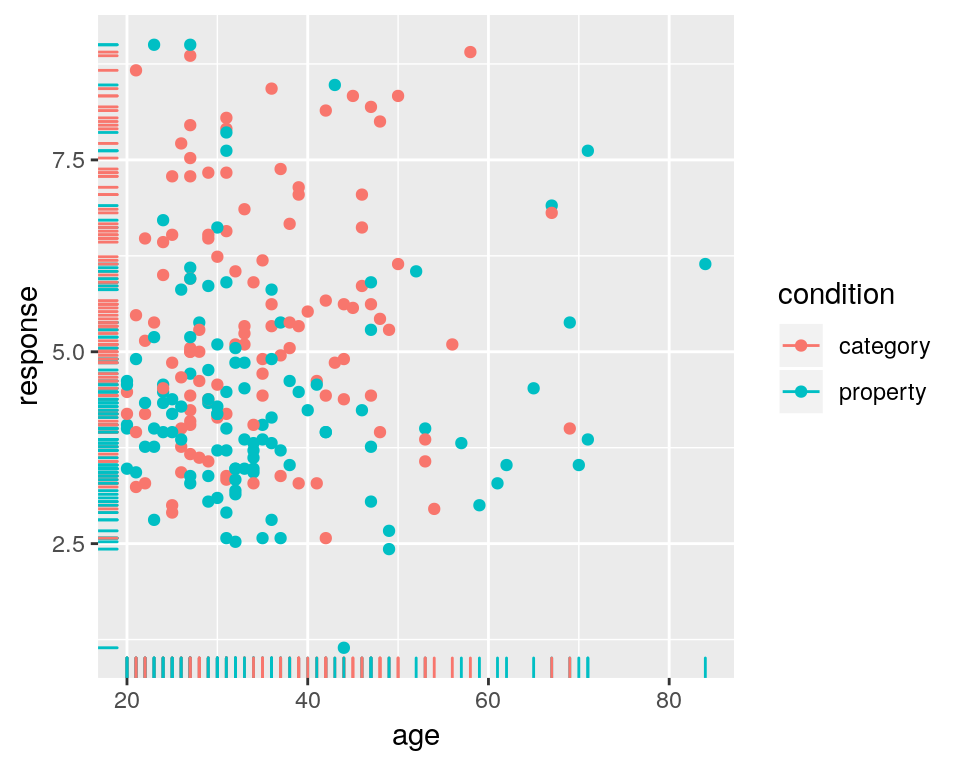
\includegraphics{2-01-visualisation_files/figure-latex/unnamed-chunk-17-1.pdf}

It's essentially the same as before, but we've switched the ordering of variables in \texttt{facet\_grid()}, added the \texttt{outlier.alpha\ =\ 0.1} argument to \texttt{geom\_boxplot()} to make the outliers fade into the background, and then specified some nicer axis titles. The resulting plot is a fair bit more readable.

As for what we're seeing in the data, there are a few different things to notice:

\begin{itemize}
\tightlist
\item
  Within every facet the responses tend to shift \emph{downwards} from left to right: as the test item becomes less similar to the training items, people are less willing to make generalisations. This pattern of similarity-based generalisation is unsurprising and it's a finding that has been replicated many, many times in the literature.
\item
  The effect of sample size is inhomogeneous. For stimuli that are very similar to the training items (test locations 1 and 2), increasing the sample size pushes the generalisation \emph{upwards}, regardless of whether category sampling or property sampling is applied
\item
  For stimuli that are very dissimilar (especially test items 6 and 7), the effect of sample size depends on the sampling method. For category sampling, basically \emph{nothing happens}: the box plots for large sample sizes aren't any different to those for small sample sizes. Yet for property sampling, there's a systematic tendency for these to shift \emph{downwards}
\end{itemize}

Assuming that these findings replicate\footnote{They appear to -- we ran 9 experiments in total and while some effects are a little fragile and I wouldn't put too much faith in their ability to replicate, the core effect in which there are systematic differences in how statistical information (e.g., sample size, base rate, auxiliary data) interacts with the sampling mechanism replicated every time; oh and if you go read the paper the model predictions correlate with human data very highly, always produce the same qualitative patterns regardless of parametre values\ldots{} etc, etc. This isn't a cognitive science paper so I won't bore you with details, but the reason this works as cleanly as it does is that we didn't choose these manipulations arbitrarily. We had a proper theory to guide us!} it looks like we have a three-way interaction of some kind!

To be honest though, I'm still not pleased with this graph. I think we can do better.

\hypertarget{bubble-plots}{%
\section{Bubble plots}\label{bubble-plots}}

One difficulty with box plots is that they only work as distributional summaries when the data are unimodal. If most people respond with extreme values, the box plot ends up being a little misleading. Violin plots are often better at capturing multimodality, but they're designed to work for continuous variables and often behave poorly when applied to data that fall in a small number of ordered categories. Psychological data from questionnaires or -- as in the \texttt{frames} data set - other ordinal response methods often have exactly this characteristic. Neither box plots nor violin plots are ideally suited to this situation.

Fortunately a bubble plot can help out here. This takes the form of a scatter plot, but instead of plotting every data point as a unique dot, we plot dots at every location whose size (area) is proportional to the number of cases at that location.\footnote{There are drawbacks to bubble plots. The psychophysical function for area isn't linear, so subjective area doesn't scale perfectly with actual area. If you need people to be able to make fine-grained comparisons between quantities don't use bubble plots. However, my goal here is different - I don't mind if we can't quite see the ``perfect'' relationship, I just want the ``gist'' to come through properly.} To do this with \textbf{ggplot2} all we need to do is use the \texttt{geom\_count()} function. When applied to the \texttt{frames} data, we get this:

\begin{Shaded}
\begin{Highlighting}[]
\NormalTok{samplingframes }\OperatorTok
\StringTok{  }\KeywordTok{ggplot}\NormalTok{(}\KeywordTok{aes}\NormalTok{(}\DataTypeTok{x =}\NormalTok{ test_item, }\DataTypeTok{y =}\NormalTok{ response)) }\OperatorTok{+}\StringTok{ }
\StringTok{  }\KeywordTok{facet_grid}\NormalTok{(condition }\OperatorTok{~}\StringTok{ }\NormalTok{sample_size) }\OperatorTok{+}
\StringTok{  }\KeywordTok{geom_count}\NormalTok{()}
\end{Highlighting}
\end{Shaded}

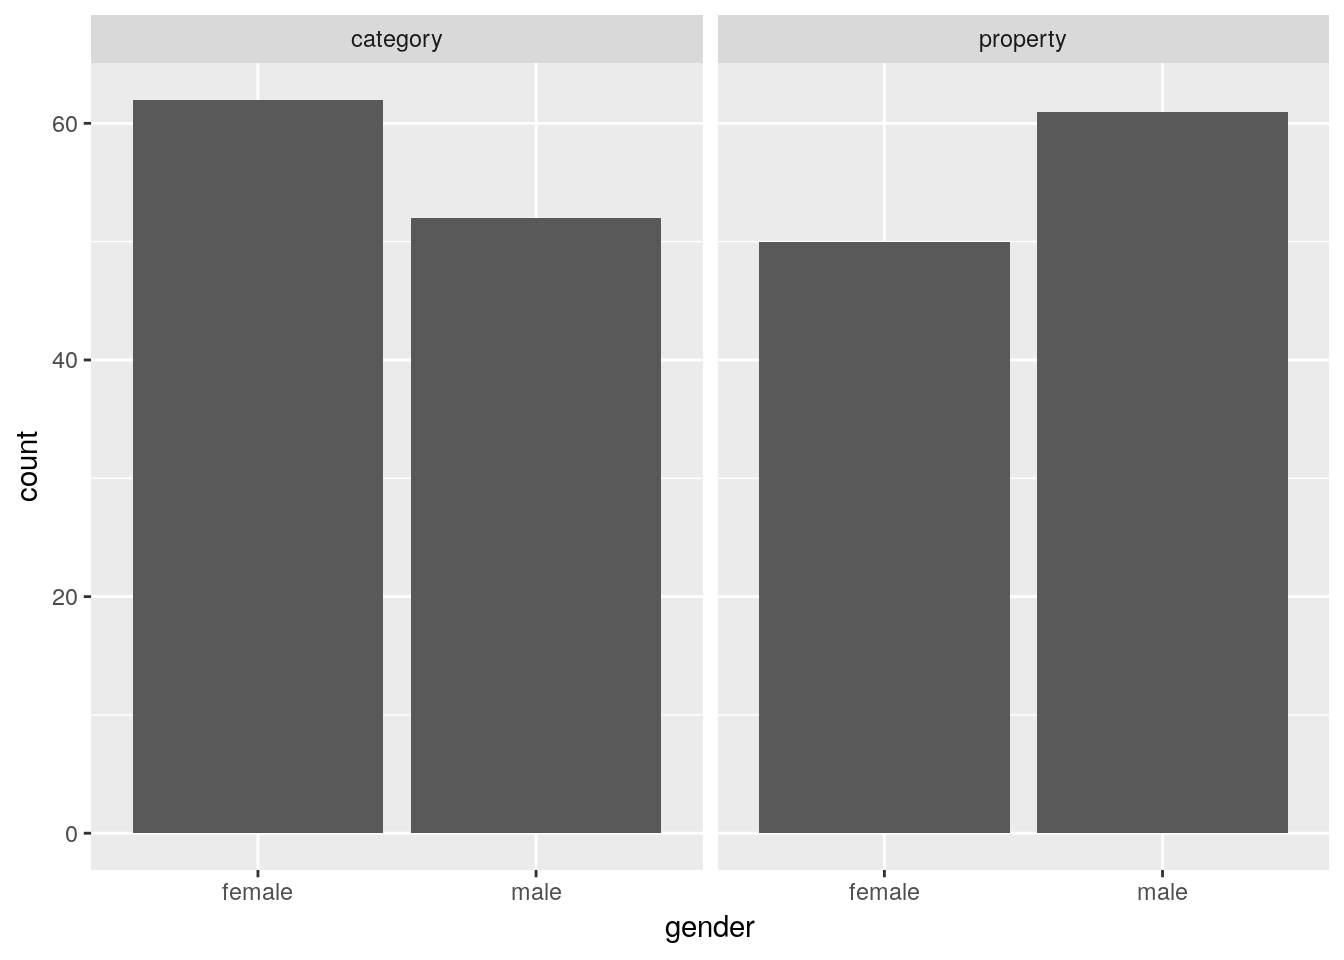
\includegraphics{2-01-visualisation_files/figure-latex/unnamed-chunk-18-1.pdf}

This version of the plot highlights a failure of the box plot version. Compare the distribution of responses to test item 7 in the category sampling condition (top row). In the \texttt{small} sample size, the modal response is 4, with most people using the middle category, whereas for the \texttt{large} sample size most people are using the extremes, responding with either 0 or 9. However, both cases have the same median and very similar inter-quartile ranges, so the box plots look almost the same!

On the other hand, this plot is a little hard to read. We've added a lot of new detail about the low frequency responses and in doing so learned more about the overall distribution of responding, but that's come at the cost of making it harder to see what the most typical responses are! A compromise that I am often fond of is using shading to slightly de-emphasize the low frequency cases. Larger bubbles should stand out (dark colour), but low frequency responses should fade into the light grey background. It's actually pretty easy to do that: \texttt{geom\_count()} keeps track of the number of observations in each cell, and so we can add a new aesthetic to the \texttt{geom\_count()} layer, simply by specifying \texttt{colour\ =\ ..n..}:

\begin{Shaded}
\begin{Highlighting}[]
\NormalTok{samplingframes }\OperatorTok
\StringTok{  }\KeywordTok{ggplot}\NormalTok{(}\KeywordTok{aes}\NormalTok{(}\DataTypeTok{x =}\NormalTok{ test_item, }\DataTypeTok{y =}\NormalTok{ response)) }\OperatorTok{+}\StringTok{ }
\StringTok{  }\KeywordTok{facet_grid}\NormalTok{(condition }\OperatorTok{~}\StringTok{ }\NormalTok{sample_size) }\OperatorTok{+}
\StringTok{  }\KeywordTok{geom_count}\NormalTok{(}\KeywordTok{aes}\NormalTok{(}\DataTypeTok{colour =}\NormalTok{ ..n..))}
\end{Highlighting}
\end{Shaded}

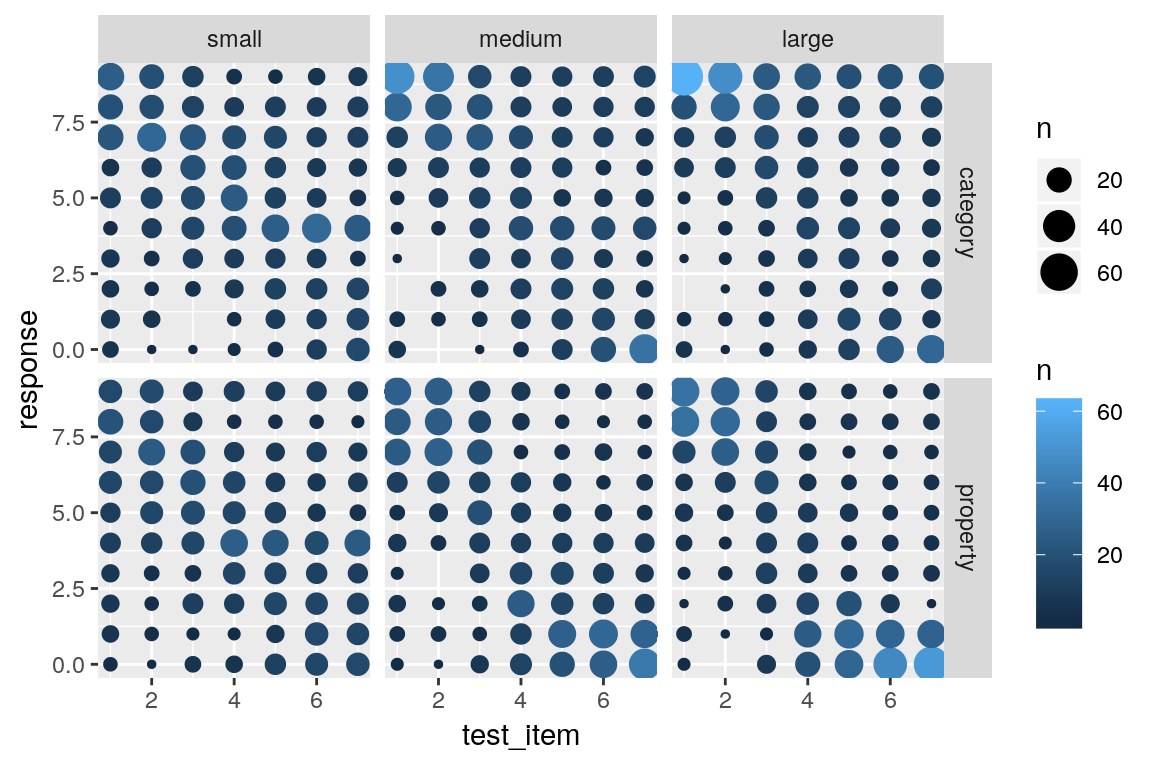
\includegraphics{2-01-visualisation_files/figure-latex/unnamed-chunk-19-1.pdf}

That's a little nicer, but in this case I don't want or need the pretty blue colouring. What I want to do is specify my own grey scale, where larger dots are coloured closer to black (e.g., upper bound is \texttt{"grey20"}) and the smaller dots are coloured in a light grey (e.g., lower bound is \texttt{"grey80"}).\footnote{R is quite flexible in how it handles colours. For most purposes you can use an English colour word and R will have a rough idea what you mean. Type \texttt{colours()} at the console to see a list of the colour names it knows: there are a lot! Alternatively you can specify a hexadecimal string like \texttt{\#88398A}, or use a function like \texttt{rgb()} or \texttt{hsv()} to construct the colour you want.} Then all I have to do is this:

\begin{Shaded}
\begin{Highlighting}[]
\NormalTok{samplingframes }\OperatorTok
\StringTok{  }\KeywordTok{ggplot}\NormalTok{(}\KeywordTok{aes}\NormalTok{(}\DataTypeTok{x =}\NormalTok{ test_item, }\DataTypeTok{y =}\NormalTok{ response)) }\OperatorTok{+}\StringTok{ }
\StringTok{  }\KeywordTok{facet_grid}\NormalTok{(condition }\OperatorTok{~}\StringTok{ }\NormalTok{sample_size) }\OperatorTok{+}
\StringTok{  }\KeywordTok{geom_count}\NormalTok{(}\KeywordTok{aes}\NormalTok{(}\DataTypeTok{colour =}\NormalTok{ ..n..)) }\OperatorTok{+}\StringTok{ }
\StringTok{  }\KeywordTok{scale_colour_gradient}\NormalTok{(}\DataTypeTok{low =} \StringTok{"grey80"}\NormalTok{, }\DataTypeTok{high =} \StringTok{"grey20"}\NormalTok{)}
\end{Highlighting}
\end{Shaded}

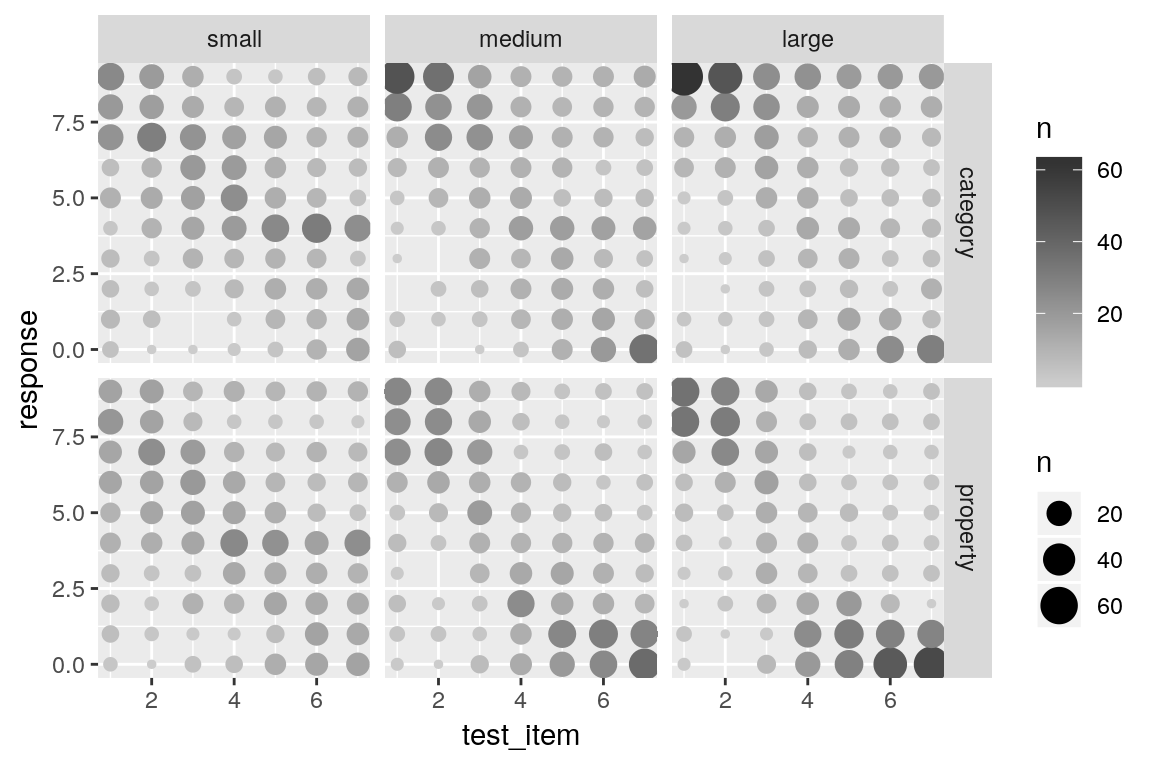
\includegraphics{2-01-visualisation_files/figure-latex/unnamed-chunk-20-1.pdf}

To my mind that's much more readable! It captures the multimodality of the responding without overwhelming the viewer with too much detail. There are still some issues that you might want to care about in real life -- the figure is a little too low contrast for people with less than perfect vision, for instance. But it comes a lot closer to what we need.

\hypertarget{error-bars}{%
\section{Error bars}\label{error-bars}}

As much as I love the bubble plot above, academic journals often expect a more compressed representation of the data, especially when the manuscript you're submitting involves a large number of experiments. It's often the case that we want to summarise the data from a single condition using a ``mean plus error bar'' style plot. A common format is to plot the mean for every experimental condition and have error bars plotting the 95\% confidence interval for the mean. To do that for the \texttt{frames} data, let's begin by constructing a summary data set

\begin{Shaded}
\begin{Highlighting}[]
\NormalTok{frames_mean <-}\StringTok{ }\NormalTok{samplingframes }\OperatorTok
\StringTok{  }\KeywordTok{group_by}\NormalTok{(condition,sample_size,test_item) }\OperatorTok
\StringTok{  }\KeywordTok{summarise}\NormalTok{(}
    \DataTypeTok{mean_response =} \KeywordTok{mean}\NormalTok{(response),}
    \DataTypeTok{lower =}\NormalTok{ lsr}\OperatorTok{::}\KeywordTok{ciMean}\NormalTok{(response)[}\DecValTok{1}\NormalTok{],}
    \DataTypeTok{upper =}\NormalTok{ lsr}\OperatorTok{::}\KeywordTok{ciMean}\NormalTok{(response)[}\DecValTok{2}\NormalTok{]}
\NormalTok{  )}
\NormalTok{frames_mean}
\end{Highlighting}
\end{Shaded}

\begin{verbatim}
## # A tibble: 42 x 6
## # Groups:   condition, sample_size [6]
##    condition sample_size test_item mean_response lower upper
##    <chr>     <fct>           <dbl>         <dbl> <dbl> <dbl>
##  1 category  small               1          6.07  5.55  6.59
##  2 category  small               2          6.26  5.84  6.69
##  3 category  small               3          5.87  5.50  6.24
##  4 category  small               4          5.11  4.74  5.49
##  5 category  small               5          4.55  4.12  4.99
##  6 category  small               6          4.16  3.69  4.63
##  7 category  small               7          3.98  3.44  4.52
##  8 category  medium              1          7.32  6.85  7.78
##  9 category  medium              2          7.17  6.80  7.54
## 10 category  medium              3          5.98  5.54  6.42
## # ... with 32 more rows
\end{verbatim}

In this case I'm using the \texttt{ciMean()} function from the \textbf{lsr} package to compute the 95\% confidence intervals. Just so that you can see how this function works -- without all the additional complications from calling it within the \texttt{summarise()} operation -- here's a simple example. I'll generate 20 numbers from a normal distribution with true mean 100 and true standard deviation 15 (following the convention used for IQ scores), and then use the \texttt{ciMean()} function to calculate a 95\% confidence interval:

\begin{Shaded}
\begin{Highlighting}[]
\NormalTok{fake_iq <-}\StringTok{ }\KeywordTok{rnorm}\NormalTok{(}\DataTypeTok{n =} \DecValTok{20}\NormalTok{, }\DataTypeTok{mean =} \DecValTok{100}\NormalTok{, }\DataTypeTok{sd =} \DecValTok{15}\NormalTok{)  }\CommentTok{# normally distributed data}
\NormalTok{lsr}\OperatorTok{::}\KeywordTok{ciMean}\NormalTok{(fake_iq)                           }\CommentTok{# 95% confidence interval }
\end{Highlighting}
\end{Shaded}

\begin{verbatim}
##             2.5%    97.5%
## fake_iq 94.36016 112.5708
\end{verbatim}

So the \texttt{lower} variable in \texttt{frames\_mean} is the lower bound on the 95\% confidence interval, and \texttt{upper} is the upper bound. In any case, now that we have data in an appropriate format we can create the plot.

To add error bars is no more difficult than anything else in \textbf{ggplot2}. There is a geom called \texttt{geom\_errorbar()} that will draw those for us. However, it does need some new information. In our previous graphs we've specifed three aesthetics at the beginning of our graphing exercise, namely \texttt{x\ =\ test\_item}, \texttt{y\ =\ mean\_response} and \texttt{colour\ =\ condition}. That works fine for \texttt{geom\_point()} because doesn't need anything else, but \texttt{geom\_errorbar()} also needs to know which variables specify the \texttt{ymin} and \texttt{ymax} values that will be displayed in the error bars. If I wanted to, I could could include these aesthetics within the original call to \texttt{ggplot()} but I'll do something a little different this time. Individual geoms can have their own unique aesthetics, so I can insert a new call to \texttt{aes()} within the \texttt{geom\_errorbar()} call. Conceptually I find this neater, because it makes clear that \texttt{ymin} and \texttt{ymax} are aesthetics that apply to the error bars, but not to other geoms in the plot. Anyway here's the command:

\begin{Shaded}
\begin{Highlighting}[]
\NormalTok{my_pic <-}\StringTok{ }\NormalTok{frames_mean }\OperatorTok
\StringTok{  }\KeywordTok{ggplot}\NormalTok{(}\KeywordTok{aes}\NormalTok{(}\DataTypeTok{x =}\NormalTok{ test_item, }\DataTypeTok{y =}\NormalTok{ mean_response, }\DataTypeTok{colour =}\NormalTok{ condition)) }\OperatorTok{+}
\StringTok{  }\KeywordTok{geom_point}\NormalTok{() }\OperatorTok{+}
\StringTok{  }\KeywordTok{geom_errorbar}\NormalTok{(}\KeywordTok{aes}\NormalTok{(}\DataTypeTok{ymin =}\NormalTok{ lower, }\DataTypeTok{ymax =}\NormalTok{ upper)) }\OperatorTok{+}\StringTok{  }\CommentTok{# add the error bars!}
\StringTok{  }\KeywordTok{facet_wrap}\NormalTok{(}\OperatorTok{~}\NormalTok{sample_size)}
\end{Highlighting}
\end{Shaded}

Hey, where's my plot? Oh right\ldots{} notice that I assigned the result to a variable called \texttt{my\_pic}. Under the hood, \texttt{my\_pic} is essentially a big list of information that specifies everything R needs to know to draw the plot. So if we want to \emph{see} the plot, all we need to do is call \texttt{print(my\_pic)} or \texttt{plot(my\_pic)}, or even more simply I can do this:

\begin{Shaded}
\begin{Highlighting}[]
\NormalTok{my_pic}
\end{Highlighting}
\end{Shaded}

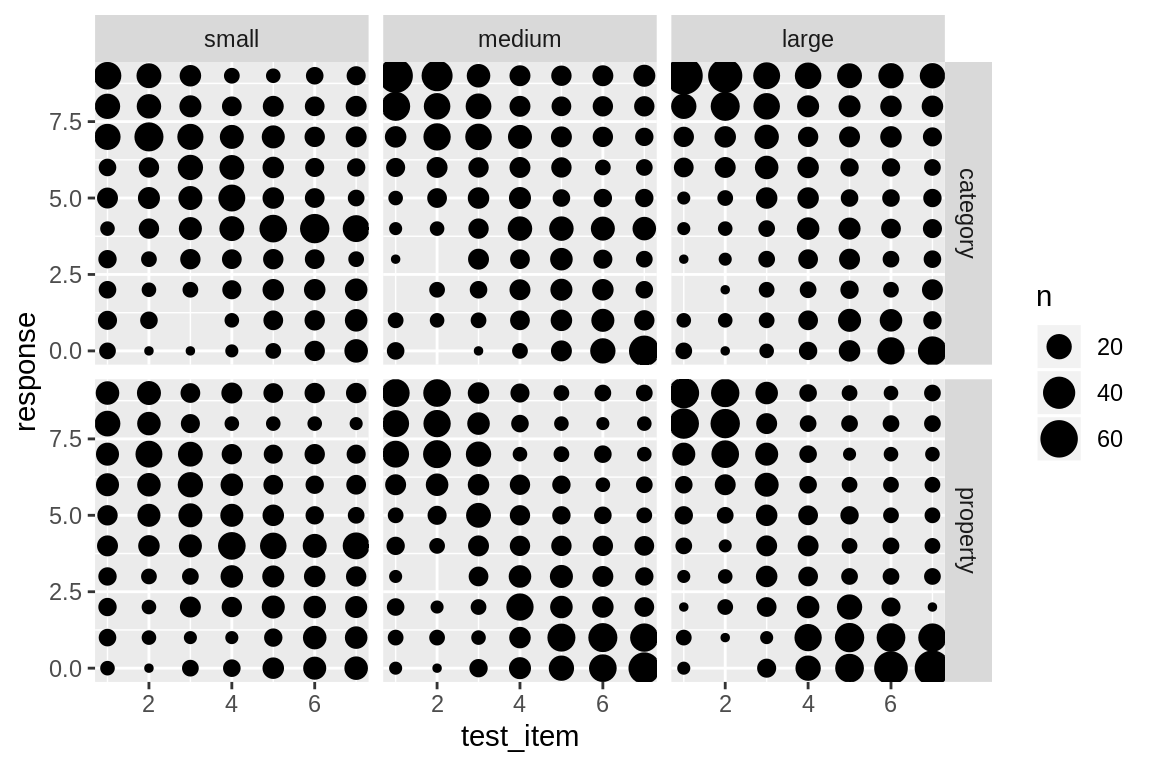
\includegraphics{2-01-visualisation_files/figure-latex/unnamed-chunk-24-1.pdf}

Clearly, when compared to the bubble plot we are losing a lot of information -- all we have left is information about the distributional mean -- but it's still fairly informative about what is going on across the diferent conditions.

Another thing worth noting. Because the test items vary along a continuous scale, it's appropriate to connect the points with lines. I can do this in a straightforward way simply by adding \texttt{geom\_line()} to the plot:

\begin{Shaded}
\begin{Highlighting}[]
\NormalTok{my_pic }\OperatorTok{+}\StringTok{ }\KeywordTok{geom_line}\NormalTok{()}
\end{Highlighting}
\end{Shaded}

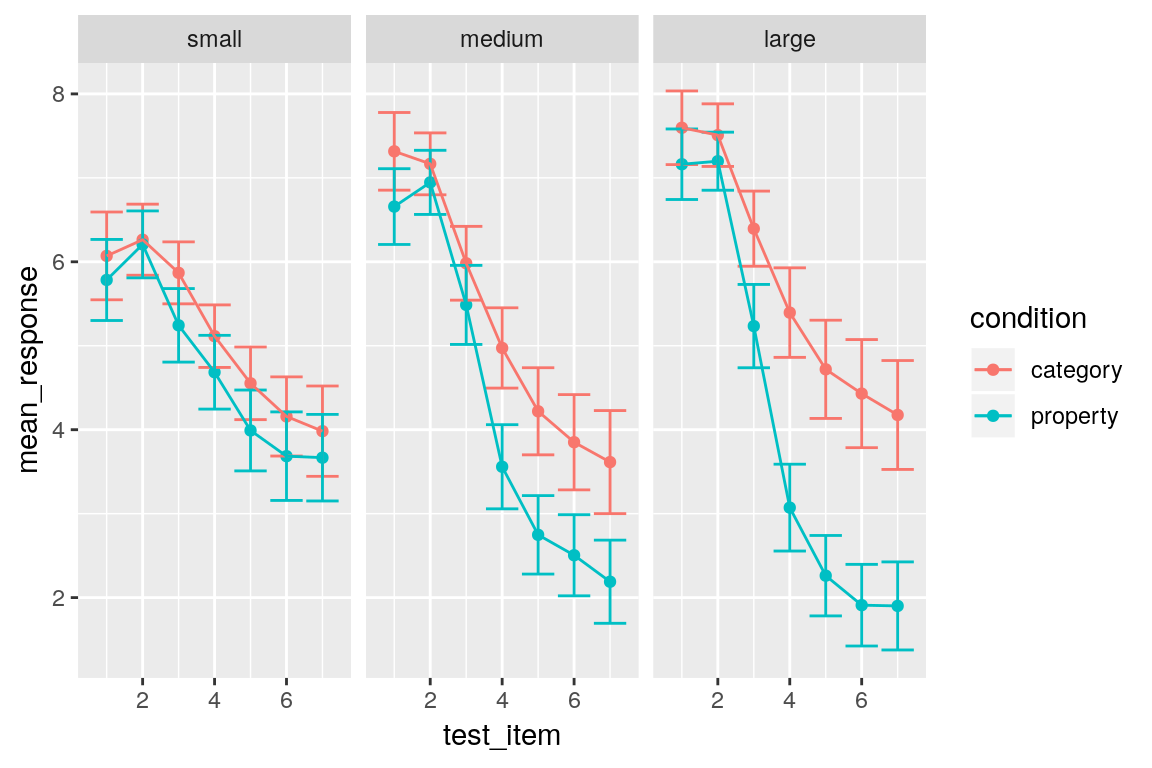
\includegraphics{2-01-visualisation_files/figure-latex/unnamed-chunk-25-1.pdf}

Notice that I can add \texttt{geom\_line()} directly to \texttt{my\_pic}. That can be extremely handy if you've worked out what the core features of your plot will be and want to play around with a few possible additions to the plot.

\hypertarget{other-possibilities}{%
\section{Other possibilities}\label{other-possibilities}}

As you can see, there are quite a few things you can do with this package. However, the \textbf{ggplot2} package provides many more plotting tools than I've described so far, and it was designed to be extensible so there are many other packages that extend it in interesting ways. Even without looking at other packages, there are various neat possibilities. Just to give you a bit of a sense of this, here are a few more! If I want to add contouring to a scatter plot, I can do this using the \texttt{geom\_density\_2d()} function:

\begin{Shaded}
\begin{Highlighting}[]
\NormalTok{frames_small }\OperatorTok\StringTok{ }
\StringTok{  }\KeywordTok{ggplot}\NormalTok{(}\DataTypeTok{mapping =} \KeywordTok{aes}\NormalTok{(}\DataTypeTok{x =}\NormalTok{ age, }\DataTypeTok{y =}\NormalTok{ response, }\DataTypeTok{colour =}\NormalTok{ condition)) }\OperatorTok{+}
\StringTok{  }\KeywordTok{geom_point}\NormalTok{() }\OperatorTok{+}\StringTok{ }
\StringTok{  }\KeywordTok{theme_bw}\NormalTok{() }\OperatorTok{+}
\StringTok{  }\KeywordTok{geom_density_2d}\NormalTok{() }\OperatorTok{+}
\StringTok{  }\KeywordTok{facet_wrap}\NormalTok{(}\OperatorTok{~}\NormalTok{condition) }\OperatorTok{+}
\StringTok{  }\KeywordTok{ylim}\NormalTok{(}\DecValTok{0}\NormalTok{,}\DecValTok{9}\NormalTok{)}
\end{Highlighting}
\end{Shaded}

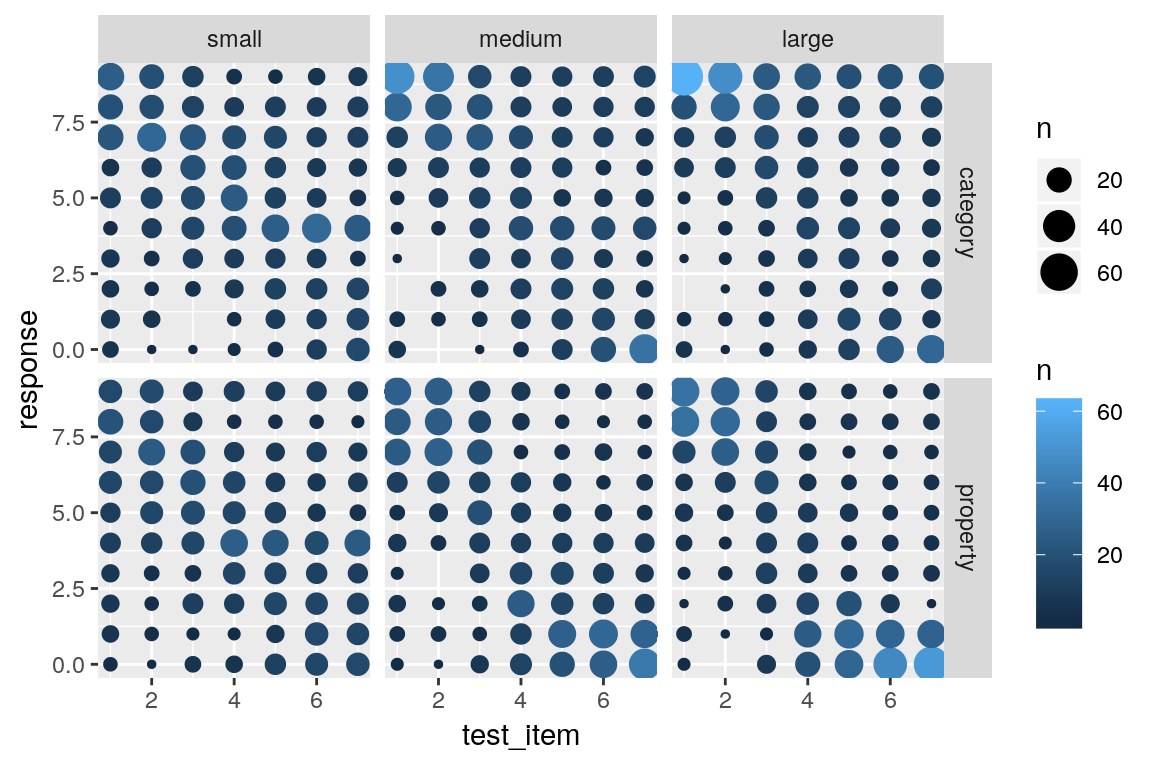
\includegraphics{2-01-visualisation_files/figure-latex/unnamed-chunk-26-1.pdf}

Alternatively, if I want to add regression lines to this plot I can use \texttt{geom\_smooth()}. By default the \texttt{geom\_smooth()} function applies a non-linear method (loess regression), which we saw previously in the \href{./prelude-to-data.html}{prelude}. This is also customisable. If I want to use a simpler linear model to provide my regression line, all I need to do is specify \texttt{method\ =\ "lm"} and I get a plot like this:

\begin{Shaded}
\begin{Highlighting}[]
\NormalTok{frames_small }\OperatorTok\StringTok{ }
\StringTok{  }\KeywordTok{ggplot}\NormalTok{(}\DataTypeTok{mapping =} \KeywordTok{aes}\NormalTok{(}\DataTypeTok{x =}\NormalTok{ age, }\DataTypeTok{y =}\NormalTok{ response, }\DataTypeTok{colour =}\NormalTok{ condition)) }\OperatorTok{+}
\StringTok{  }\KeywordTok{geom_point}\NormalTok{() }\OperatorTok{+}\StringTok{ }
\StringTok{  }\KeywordTok{geom_smooth}\NormalTok{(}\DataTypeTok{method =} \StringTok{"lm"}\NormalTok{) }\OperatorTok{+}
\StringTok{  }\KeywordTok{facet_wrap}\NormalTok{(}\OperatorTok{~}\NormalTok{condition) }\OperatorTok{+}
\StringTok{  }\KeywordTok{ylim}\NormalTok{(}\DecValTok{0}\NormalTok{,}\DecValTok{9}\NormalTok{)}
\end{Highlighting}
\end{Shaded}

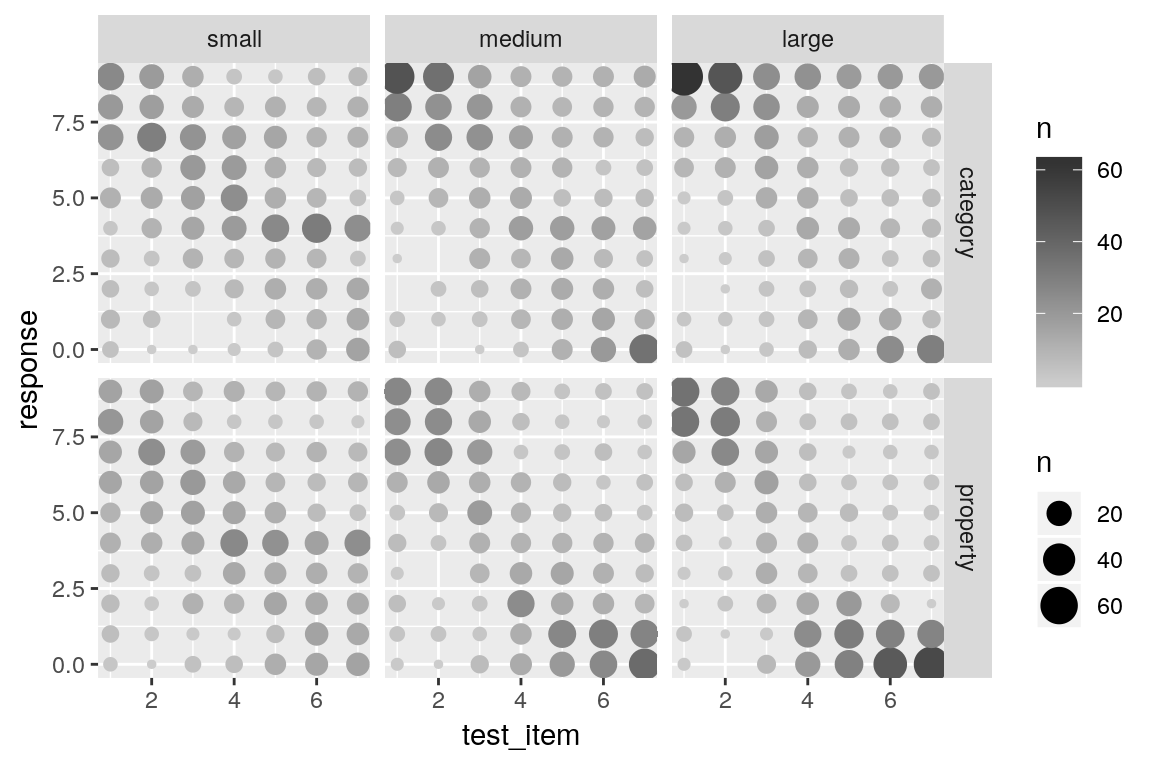
\includegraphics{2-01-visualisation_files/figure-latex/unnamed-chunk-27-1.pdf}

Similarly, plots are customisable in other ways. We can use \texttt{theme\_dark()} to switch to a dark theme or \texttt{theme\_bw()} to switch to a black and white scheme. We can add horizontal lines to plots with \texttt{geom\_hline()}, vertical lines with \texttt{geom\_vline()} and diagonal lines with \texttt{geom\_abline()}. The colour palette can be adapted in arbitrary ways (e.g.~with \texttt{scale\_color\_brewer}). We can control the axis scales with \texttt{xlim()} and \texttt{ylim()}. We can add text to a plot with \texttt{geom\_text()}. Here's an example showing some of those customisation:

\begin{Shaded}
\begin{Highlighting}[]
\NormalTok{my_new_pic <-}\StringTok{ }\NormalTok{my_pic }\OperatorTok{+}\StringTok{ }
\StringTok{  }\KeywordTok{theme_dark}\NormalTok{() }\OperatorTok{+}
\StringTok{  }\KeywordTok{scale_color_brewer}\NormalTok{(}\DataTypeTok{palette =} \StringTok{"Pastel2"}\NormalTok{) }\OperatorTok{+}
\StringTok{  }\KeywordTok{ylim}\NormalTok{(}\DecValTok{0}\NormalTok{, }\DecValTok{9}\NormalTok{) }\OperatorTok{+}\StringTok{ }
\StringTok{  }\KeywordTok{geom_vline}\NormalTok{(}\DataTypeTok{xintercept =} \FloatTok{2.5}\NormalTok{, }\DataTypeTok{colour =} \StringTok{"white"}\NormalTok{, }\DataTypeTok{lty =} \StringTok{"dotted"}\NormalTok{) }\OperatorTok{+}
\StringTok{  }\KeywordTok{xlab}\NormalTok{(}\StringTok{"Location of Test Stimulus"}\NormalTok{) }\OperatorTok{+}
\StringTok{  }\KeywordTok{ylab}\NormalTok{(}\StringTok{"Mean Response"}\NormalTok{)}

\NormalTok{my_new_pic}
\end{Highlighting}
\end{Shaded}

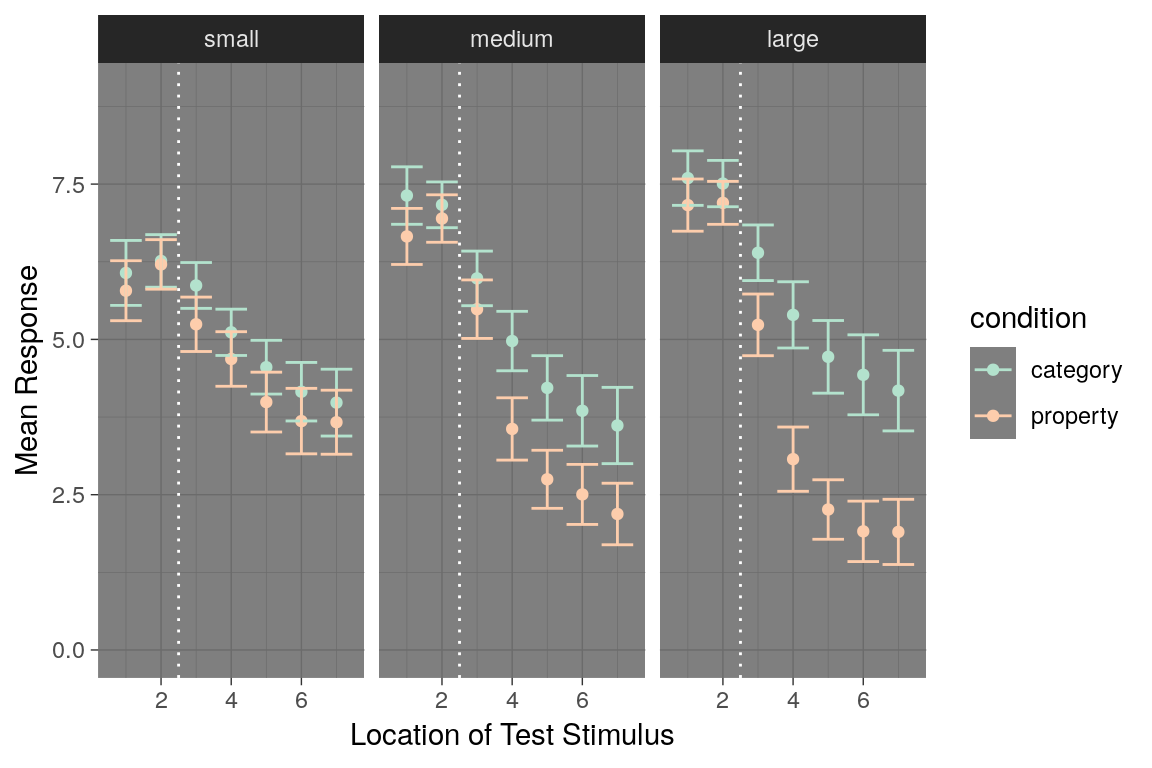
\includegraphics{2-01-visualisation_files/figure-latex/unnamed-chunk-28-1.pdf}

The possibilities are limited mostly by your imagination, and by common sense. The \textbf{ggplot2} system is so rich and flexible that it's easy to go overboard with creating pretty pictures. Always remember that there's a human reader at the other end of your picture, and they're more interested in what your data visualisation can tell them about \emph{the data}, not what it says about your R skills! :-)

\hypertarget{saving-images}{%
\section{Saving images}\label{saving-images}}

The last topic I want to cover here is how to save your plot to an image file. Suppose I want to take \texttt{my\_new\_plot} and save it to a PNG file that is 16cm wide and 8cm high. The \texttt{ggsave()} function allows me to do that, and the command is pretty intuitive:

\begin{Shaded}
\begin{Highlighting}[]
\KeywordTok{ggsave}\NormalTok{(}
  \DataTypeTok{filename =} \StringTok{"./output/frame_pic.png"}\NormalTok{,}
  \DataTypeTok{plot =}\NormalTok{ my_new_pic,}
  \DataTypeTok{width =} \DecValTok{16}\NormalTok{,}
  \DataTypeTok{height =} \DecValTok{8}\NormalTok{,}
  \DataTypeTok{units =} \StringTok{"cm"}
\NormalTok{)}
\end{Highlighting}
\end{Shaded}

The function is smart enough to guess from the \texttt{filename} argument what kind of image file to create (e.g., PNG, JPG, etc), and so as long as the filename specifies a file extension that \texttt{ggsave()} can handle it will automatically create the right kind of image. The result in this case is \href{./output/frame_pic.png}{this image file}.

\hypertarget{further-reading}{%
\section{Further reading}\label{further-reading}}

\begin{itemize}
\tightlist
\item
  \href{https://socviz.co/}{Data visualisation: A practical introduction}. Kieran Healy
\item
  ggplot2: Elegant graphics for data analysis. Hadley Wickham.
\end{itemize}

\hypertarget{descriptives}{%
\chapter{Describing data}\label{descriptives}}

\begin{itemize}
\tightlist
\item
  Explain summary statistics
\item
  Cover basic dplyr
\end{itemize}

\hypertarget{part-learning-from-data}{%
\part{Learning from data}\label{part-learning-from-data}}

\hypertarget{probability}{%
\chapter{Probability}\label{probability}}

\hypertarget{orthodox}{%
\chapter{Orthodox theory}\label{orthodox}}

\hypertarget{bayes}{%
\chapter{Bayesian theory}\label{bayes}}

\hypertarget{linearmodels}{%
\chapter{Linear models}\label{linearmodels}}

\hypertarget{part-tools-of-the-trade}{%
\part{Tools of the trade}\label{part-tools-of-the-trade}}

\hypertarget{cleaning-data}{%
\chapter{Cleaning data}\label{cleaning-data}}

\begin{itemize}
\tightlist
\item
  Reshaping
\item
  Joins
\item
  Looking for errors
\item
  Tidy data
\item
  Naming things
\item
  etc
\end{itemize}

\hypertarget{documenting}{%
\chapter{Documenting your work}\label{documenting}}

\begin{itemize}
\tightlist
\item
  readmes, rmarkdowns, packages
\item
  preregistration methods
\item
  version control (super brief?)
\item
  data archiving
\end{itemize}

\hypertarget{appendix-appendices}{%
\appendix}


\hypertarget{data-types}{%
\chapter{Data types in R}\label{data-types}}

\begin{quote}
He divided the universe in forty categories or classes, these being further subdivided into differences, which was then subdivided into species. He assigned to each class a monosyllable of two letters; to each difference, a consonant; to each species, a vowel. For example: \texttt{de}, which means an element; \texttt{deb}, the first of the elements, fire; \texttt{deba}, a part of the element fire, a flame. \ldots{} The words of the analytical language created by John Wilkins are not mere arbitrary symbols; each letter in them has a meaning, like those from the Holy Writ had for the Cabbalists.
~~~~~~--Jorge Luis Borges, \href{https://en.wikipedia.org/wiki/The_Analytical_Language_of_John_Wilkins}{The Analytical Language of John Wilkins}
\end{quote}

\begin{Shaded}
\begin{Highlighting}[]
\KeywordTok{library}\NormalTok{(tidyverse)}
\KeywordTok{library}\NormalTok{(tidylsr)}
\end{Highlighting}
\end{Shaded}

\hypertarget{vectors}{%
\section{Vectors}\label{vectors}}

When I introduced variablesx, I showed you how we can use them to store a single number. In this section, we'll extend this idea and look at how to store multiple numbers within the one variable. In R the name for a variable that can store multiple values is a \textbf{vector}. So let's create one.

\hypertarget{character-vectors}{%
\subsection{Character vectors}\label{character-vectors}}

Let's return to the example we were working with in the previous section on variables. We're designing a survey, and we want to keep track of the responses that a participant has given. This time, let's imagine that we've finished running the survey and we're examining the data. Suppose we've administered the \href{http://www2.psy.unsw.edu.au/dass/}{Depression, Anxiety and Stress Scale} (DASS) and as a consequence every participant has scores for on the \emph{depression}, \emph{anxiety} and \emph{stress} scales provided by the DASS. One thing we might want to do is create a single variable called \texttt{scale\_name} that identifies the three scales. The simplest way to do this in R is to use the \emph{combine} function, \texttt{c}.\footnote{Notice that I didn't specify any argument names here. The \texttt{c} function is one of those cases where we don't use names. We just type all the numbers, and R just dumps them all in a single variable.} To do so, all we have to do is type the values we want to store in a comma separated list, like this

\begin{Shaded}
\begin{Highlighting}[]
\NormalTok{scale_name <-}\StringTok{ }\KeywordTok{c}\NormalTok{(}\StringTok{"depression"}\NormalTok{,}\StringTok{"anxpiety"}\NormalTok{,}\StringTok{"stress"}\NormalTok{)}
\NormalTok{scale_name}
\end{Highlighting}
\end{Shaded}

\begin{verbatim}
## [1] "depression" "anxpiety"   "stress"
\end{verbatim}

To use the correct terminology here, we have a single variable here called \texttt{scale\_name}: this variable is a \textbf{vector} that has three \textbf{elements}.
Because the vector contains text, it is a character vector. You can use the \texttt{length} function to check the length, and the \texttt{class} function to check what kind of vector it is:

\begin{Shaded}
\begin{Highlighting}[]
\KeywordTok{length}\NormalTok{(scale_name)}
\end{Highlighting}
\end{Shaded}

\begin{verbatim}
## [1] 3
\end{verbatim}

\begin{Shaded}
\begin{Highlighting}[]
\KeywordTok{class}\NormalTok{(scale_name)}
\end{Highlighting}
\end{Shaded}

\begin{verbatim}
## [1] "character"
\end{verbatim}

\hypertarget{numeric-vectors}{%
\subsection{Numeric vectors}\label{numeric-vectors}}

As you might expect, we can define numeric or logical variables in the same way. For instance, we could define the raw scores on the three DASS scales like so:

\begin{Shaded}
\begin{Highlighting}[]
\NormalTok{raw_score <-}\StringTok{ }\KeywordTok{c}\NormalTok{(}\DecValTok{12}\NormalTok{, }\DecValTok{3}\NormalTok{, }\DecValTok{8}\NormalTok{)}
\NormalTok{raw_score}
\end{Highlighting}
\end{Shaded}

\begin{verbatim}
## [1] 12  3  8
\end{verbatim}

We'll talk about logical vectors in a moment.

\hypertarget{extracting-an-element}{%
\subsection{Extracting an element}\label{extracting-an-element}}

If I want to extract the first element from the vector, all I have to do is refer to the relevant numerical index, using square brackets to do so. For example, to get the first element of \texttt{scale\_name} I would type this

\begin{Shaded}
\begin{Highlighting}[]
\NormalTok{scale_name[}\DecValTok{1}\NormalTok{]}
\end{Highlighting}
\end{Shaded}

\begin{verbatim}
## [1] "depression"
\end{verbatim}

The second element of the vector is

\begin{Shaded}
\begin{Highlighting}[]
\NormalTok{scale_name[}\DecValTok{2}\NormalTok{]}
\end{Highlighting}
\end{Shaded}

\begin{verbatim}
## [1] "anxpiety"
\end{verbatim}

You get the idea.\footnote{Note that the square brackets here are used to index the elements of the vector, and that this is the same notation that we see in the R output. That's not accidental: when R prints \texttt{{[}1{]}\ "depression"} to the screen what it's saying is that \texttt{"depression"} is the first element of the output. When the output is long enough, you'll often see other numbers at the start of each line of the output.}

\hypertarget{extracting-multiple-elements}{%
\subsection{Extracting multiple elements}\label{extracting-multiple-elements}}

There are a few ways to extract multiple elements of a vector. The first way is to specify a vector that contains the indices of the variables that you want to keep. To extract the first two scale names:

\begin{Shaded}
\begin{Highlighting}[]
\NormalTok{scale_name[}\KeywordTok{c}\NormalTok{(}\DecValTok{1}\NormalTok{,}\DecValTok{2}\NormalTok{)]}
\end{Highlighting}
\end{Shaded}

\begin{verbatim}
## [1] "depression" "anxpiety"
\end{verbatim}

Alternatively, R provides a convenient shorthand notation in which \texttt{1:2} is a vector containing the nubmers from 1 to 2, and similarly \texttt{1:10} is a vector containing the numbers from 1 to 10. So this is also the same:

\begin{Shaded}
\begin{Highlighting}[]
\NormalTok{scale_name[}\DecValTok{1}\OperatorTok{:}\DecValTok{2}\NormalTok{]}
\end{Highlighting}
\end{Shaded}

\begin{verbatim}
## [1] "depression" "anxpiety"
\end{verbatim}

Notice that order matters here. So if I do this

\begin{Shaded}
\begin{Highlighting}[]
\NormalTok{scale_name[}\KeywordTok{c}\NormalTok{(}\DecValTok{2}\NormalTok{,}\DecValTok{1}\NormalTok{)]}
\end{Highlighting}
\end{Shaded}

\begin{verbatim}
## [1] "anxpiety"   "depression"
\end{verbatim}

I get the same numbers, but in the reverse order.

\hypertarget{removing-elements}{%
\subsection{Removing elements}\label{removing-elements}}

Finally, when working with vectors, R allows us to use negative numbers to indicate which elements to remove. So this is yet another way of doing the same thing:

\begin{Shaded}
\begin{Highlighting}[]
\NormalTok{scale_name[}\OperatorTok{-}\DecValTok{3}\NormalTok{]}
\end{Highlighting}
\end{Shaded}

\begin{verbatim}
## [1] "depression" "anxpiety"
\end{verbatim}

Notice that done of this has changed the original variable. The \texttt{scale\_name} itself has remained completely untouched.

\begin{Shaded}
\begin{Highlighting}[]
\NormalTok{scale_name}
\end{Highlighting}
\end{Shaded}

\begin{verbatim}
## [1] "depression" "anxpiety"   "stress"
\end{verbatim}

\hypertarget{editing-vectors}{%
\subsection{Editing vectors}\label{editing-vectors}}

Sometimes you'll want to change the values stored in a vector. Imagine my surprise when a student points out that \texttt{"anxpiety"} is not in fact a real thing. I should probably fix that! One possibility would be to assign the whole vector again from the beginning, using \texttt{c}. But that's a lot of typing. Also, it's a little wasteful: why should R have to redefine the names for all three scales, when only the second one is wrong? Fortunately, we can tell R to change only the second element, using this trick:

\begin{Shaded}
\begin{Highlighting}[]
\NormalTok{scale_name[}\DecValTok{2}\NormalTok{] <-}\StringTok{ "anxiety"}
\NormalTok{scale_name}
\end{Highlighting}
\end{Shaded}

\begin{verbatim}
## [1] "depression" "anxiety"    "stress"
\end{verbatim}

That's better.

Another way to edit variables in is to use the \texttt{edit} function. I won't go into that here, but if you're curious, try typing a command like this:

\begin{Shaded}
\begin{Highlighting}[]
\KeywordTok{edit}\NormalTok{(scale_name)}
\end{Highlighting}
\end{Shaded}

\hypertarget{naming-elements}{%
\subsection{Naming elements}\label{naming-elements}}

One very handy thing in R is that it lets you assign meaningul \emph{names} to the different elements in a vector. For example, the \texttt{raw\_scores} vector that we introduced earlier contains the actual data from a study but when you print it out on its own

\begin{Shaded}
\begin{Highlighting}[]
\NormalTok{raw_score}
\end{Highlighting}
\end{Shaded}

\begin{verbatim}
## [1] 12  3  8
\end{verbatim}

its not obvious what each of the scores corresponds to. There are several different ways of making this a little more meaningful (and we'll talk about them later) but for now I want to show one simple trick. Ideally, what we'd like to do is have R remember that the first element of the \texttt{raw\_score} is the ``depression'' score, the second is ``anxiety'' and the third is ``stress''. We can do that like this:

\begin{Shaded}
\begin{Highlighting}[]
\KeywordTok{names}\NormalTok{(raw_score) <-}\StringTok{ }\NormalTok{scale_name}
\end{Highlighting}
\end{Shaded}

This is a bit of an unusual looking assignment statement. Usually, whenever we use \texttt{\textless{}-} the thing on the left hand side is the variable itself (i.e., \texttt{raw\_score}) but this time around the left hand side refers to the names. To see what this command has done, let's get R to print out the \texttt{raw\_score} variable now:

\begin{Shaded}
\begin{Highlighting}[]
\NormalTok{raw_score}
\end{Highlighting}
\end{Shaded}

\begin{verbatim}
## depression    anxiety     stress 
##         12          3          8
\end{verbatim}

That's a little nicer. Element names don't just look nice, they're functional too. You can refer to the elements of a vector using their names, like so:

\begin{Shaded}
\begin{Highlighting}[]
\NormalTok{raw_score[}\StringTok{"anxiety"}\NormalTok{]}
\end{Highlighting}
\end{Shaded}

\begin{verbatim}
## anxiety 
##       3
\end{verbatim}

\hypertarget{vector-operations}{%
\subsection{Vector operations}\label{vector-operations}}

One really nice thing about vectors is that a lot of R functions and operators will work on the whole vector at once. For instance, suppose I want to normalise the raw scores from the DASS. Each scale of the DASS is constructed from 14 questions that are rated on a 0-3 scale, so the minimum possible score is 0 and the maximum is 42. Suppose I wanted to rescale the raw scores to lie on a scale from 0 to 1. I can create the \texttt{scaled\_score} variable like this:

\begin{Shaded}
\begin{Highlighting}[]
\NormalTok{scaled_score <-}\StringTok{ }\NormalTok{raw_score }\OperatorTok{/}\StringTok{ }\DecValTok{42}
\NormalTok{scaled_score}
\end{Highlighting}
\end{Shaded}

\begin{verbatim}
## depression    anxiety     stress 
## 0.28571429 0.07142857 0.19047619
\end{verbatim}

In other words, when you divide a vector by a single number, all elements in the vector get divided. The same is true for addition, subtraction, multiplicattion and taking powers. So that's neat.

Suppose it later turned out that I'd made a mistake. I hadn't in fact administered the complete DASS, only the first page. As noted in the DASS website, it's possible to fix this mistake (sort of). First, I have to recognise that my scores are actually out of 21 not 42, so the calculation I should have done is this:

\begin{Shaded}
\begin{Highlighting}[]
\NormalTok{scaled_score <-}\StringTok{ }\NormalTok{raw_score }\OperatorTok{/}\StringTok{ }\DecValTok{21}
\NormalTok{scaled_score}
\end{Highlighting}
\end{Shaded}

\begin{verbatim}
## depression    anxiety     stress 
##  0.5714286  0.1428571  0.3809524
\end{verbatim}

Then, it turns out that page 1 of the full DASS is \emph{almost} the same as the short form of the DASS, but there's a \href{http://www2.psy.unsw.edu.au/dass/DASSFAQ.htm\#_28.__I_accidentally_administered_th}{correction factor} you have to apply. The depression score needs to be multiplied by 1.04645, the anxiety score by 1.02284, and stress by 0.98617

\begin{Shaded}
\begin{Highlighting}[]
\NormalTok{correction_factor <-}\StringTok{ }\KeywordTok{c}\NormalTok{(}\FloatTok{1.04645}\NormalTok{, }\FloatTok{1.02284}\NormalTok{, }\FloatTok{0.98617}\NormalTok{)}
\NormalTok{corrected_score <-}\StringTok{ }\NormalTok{scaled_score }\OperatorTok{*}\StringTok{ }\NormalTok{correction_factor}
\NormalTok{corrected_score}
\end{Highlighting}
\end{Shaded}

\begin{verbatim}
## depression    anxiety     stress 
##  0.5979714  0.1461200  0.3756838
\end{verbatim}

What this has done is multiply the first element of \texttt{scaled\_score} by the first element of \texttt{correction\_factor}, multiply the second element of \texttt{scaled\_score} by the second element of \texttt{correction\_factor}, and so on.

I'll talk more about calculations involving vectors later, because they come up a lot. In particular R has a thing called the \emph{recycling rule} that is worth knowing about.\footnote{The recycling rule: if two vectors are of unequal length, the values of shorter one will be ``recycled''. To get a feel for how this works, try setting \texttt{x\ \textless{}-\ c(1,1,1,1,1)} and \texttt{y\ \textless{}-\ c(2,7)} and then getting R to evaluate \texttt{x\ +\ y}} But that's enough detail for now.

\hypertarget{logical-vectors}{%
\subsection{Logical vectors}\label{logical-vectors}}

I mentioned earlier that we can define vectors of logical values in the same way that we can store vectors of numbers and vectors of text, again using the \texttt{c} function to combine multiple values. Logical vectors can be useful as data in their own right, but the thing that they're expecially useful for is extracting elements of another vector, which is referred to as \emph{logical indexing}.

Here's a simple example. Suppose I decide that the stress scale is not very useful for my study, and I only want to keep the first two elements, depression and anxiety. One way to do this is to define a logical vector that indicates which values to \texttt{keep}:

\begin{Shaded}
\begin{Highlighting}[]
\NormalTok{keep <-}\StringTok{ }\KeywordTok{c}\NormalTok{(}\OtherTok{TRUE}\NormalTok{, }\OtherTok{TRUE}\NormalTok{, }\OtherTok{FALSE}\NormalTok{) }
\NormalTok{keep}
\end{Highlighting}
\end{Shaded}

\begin{verbatim}
## [1]  TRUE  TRUE FALSE
\end{verbatim}

In this instance the \texttt{keep} vector indicates that it is \texttt{TRUE} that I want to retain the first two elements, and \texttt{FALSE} that I want to keep the third. So if I type this

\begin{Shaded}
\begin{Highlighting}[]
\NormalTok{corrected_score[keep]}
\end{Highlighting}
\end{Shaded}

\begin{verbatim}
## depression    anxiety 
##  0.5979714  0.1461200
\end{verbatim}

R prints out the corrected scores for the two variables only. As usual, note that this hasn't changed the original variable. If I print out the original vector\ldots{}

\begin{Shaded}
\begin{Highlighting}[]
\NormalTok{corrected_score}
\end{Highlighting}
\end{Shaded}

\begin{verbatim}
## depression    anxiety     stress 
##  0.5979714  0.1461200  0.3756838
\end{verbatim}

\ldots{} all three values are still there. If I \emph{do} want to create a new variable, I need to explicitly assign the results of my previous command to a variable.

Let's suppose that I want to call the new variable \texttt{short\_score}, indicating that I've only retained some of the scales. Here's how I do that:

\begin{Shaded}
\begin{Highlighting}[]
\NormalTok{short_score <-}\StringTok{ }\NormalTok{corrected_score[keep]}
\NormalTok{short_score}
\end{Highlighting}
\end{Shaded}

\begin{verbatim}
## depression    anxiety 
##  0.5979714  0.1461200
\end{verbatim}

\hypertarget{comment}{%
\subsection{Comment}\label{comment}}

At this point, I hope you can see why logical indexing is such a useful thing. It's a very basic, yet very powerful way to manipulate data. For intance, I might want to extract the scores of the adult participants in a study, which would probably involve a command like \texttt{scores{[}age\ \textgreater{}\ 18{]}}. The operation \texttt{age\ \textgreater{}\ 18} would return a vector of \texttt{TRUE} and \texttt{FALSE} values, and so the the full command \texttt{scores{[}age\ \textgreater{}\ 18{]}} would return only the \texttt{scores} for participants with \texttt{age\ \textgreater{}\ 18}. It does take practice to become completely comfortable using logical indexing, so it's a good idea to play around with these sorts of commands. Practice makes perfect, and it's only by practicing logical indexing that you'll perfect the art of yelling frustrated insults at your computer.

\hypertarget{exercises-1}{%
\subsection{Exercises}\label{exercises-1}}

\begin{itemize}
\tightlist
\item
  Use the combine function \texttt{c} to create a numeric vector called \texttt{age} that lists the ages of four people (e.g., 19, 34, 7 and 67)
\item
  Use the square brackets \texttt{{[}{]}} to print out the \texttt{age} of the second person.
\item
  Use the square brackets \texttt{{[}{]}} to print out the \texttt{age} of the second person and third persons
\item
  Use the combine function \texttt{c} to create a character vector called \texttt{gender} that lists the gender of those four people
\item
  Create a logical vector \texttt{adult} that indicates whether each participant was 18 or older. Instead of using \texttt{c}, try using a logical operator like \texttt{\textgreater{}} or \texttt{\textgreater{}=} to automatically create \texttt{adult} from \texttt{age}
\item
  Test your logical indexing skills. Print out the \texttt{gender} of all the \texttt{adult} participants.
\end{itemize}

\hypertarget{factors}{%
\section{Factors}\label{factors}}

As psychological research methodology classes are at pains to point out, the data we analyse come in different kinds. Some variables are inherently \emph{quantitative} in nature: response time (RT) for instance, has a natural interpretation in units of time. So when I defined a response time variable in the previous section, I used a numeric vector. To keep my variable names concise, I'll define the same variable again using the conventional RT abbreviation:

\begin{Shaded}
\begin{Highlighting}[]
\NormalTok{RT <-}\StringTok{ }\KeywordTok{c}\NormalTok{(}\DecValTok{420}\NormalTok{, }\DecValTok{619}\NormalTok{, }\DecValTok{550}\NormalTok{, }\DecValTok{521}\NormalTok{, }\DecValTok{1003}\NormalTok{, }\DecValTok{486}\NormalTok{, }\DecValTok{512}\NormalTok{, }\DecValTok{560}\NormalTok{, }\DecValTok{495}\NormalTok{, }\DecValTok{610}\NormalTok{)}
\end{Highlighting}
\end{Shaded}

A response time of 1500 milliseconds is indeed 400 milliseconds slower than a response time of 1100 milliseconds, so addition and subtraction are meaningful operations. Similarly, 1500 milliseconds is twice as long as 750 milliseconds, so multiplication and division are also meaningful. That's not the case for other kinds of data, and this is where \textbf{factors} can be useful\ldots{}

\hypertarget{unordered-factors}{%
\subsection{Unordered factors}\label{unordered-factors}}

Some variables are inherently \emph{nominal} in nature. If I recruit participants in an online experiment I might see that their place of residence falls in one of several different regions. For simplicity, let's imagine that my study is designed to sample people from one of four distinct geographical regions: the United States, India, China or the European Union, which I'll represent using the codes \texttt{"us"}, \texttt{"in"}, \texttt{"ch"} and \texttt{"eu"}. My first thought would be to represent the data using a character vector:

\begin{Shaded}
\begin{Highlighting}[]
\NormalTok{region_raw <-}\StringTok{ }\KeywordTok{c}\NormalTok{(}\StringTok{"us"}\NormalTok{,}\StringTok{"us"}\NormalTok{,}\StringTok{"us"}\NormalTok{,}\StringTok{"eu"}\NormalTok{,}\StringTok{"in"}\NormalTok{,}\StringTok{"eu"}\NormalTok{,}\StringTok{"in"}\NormalTok{,}\StringTok{"in"}\NormalTok{,}\StringTok{"us"}\NormalTok{,}\StringTok{"in"}\NormalTok{)}
\end{Highlighting}
\end{Shaded}

This seems quite reasonable, but there's a problem: as it happens there is nobody from China in this sample. So if I try to construct a frequency table of these data -- which I can do using the \texttt{table()} function in R -- the answer I get omits China entirely:

\begin{Shaded}
\begin{Highlighting}[]
\KeywordTok{table}\NormalTok{(region_raw)}
\end{Highlighting}
\end{Shaded}

\begin{verbatim}
## region_raw
## eu in us 
##  2  4  4
\end{verbatim}

Intuitively it feels like there should be a fourth entry here, indicating that we have 0 participants from China. R has a natural tool for representing this idea, called a \textbf{factor}. First, we'll create a new variable using the \texttt{factor()} function that contains the same information but represents it as a factor:

\begin{Shaded}
\begin{Highlighting}[]
\NormalTok{region <-}\StringTok{ }\KeywordTok{factor}\NormalTok{(region_raw)}
\NormalTok{region}
\end{Highlighting}
\end{Shaded}

\begin{verbatim}
##  [1] us us us eu in eu in in us in
## Levels: eu in us
\end{verbatim}

This looks a much the same, and not surprisingly R still doesn't know anything about the possibility of participants from China. However, notice that the bottom of the output lists the \emph{levels} of the factor. The levels of a factor specify the set of values that variable could have taken. By default, \texttt{factor()} tries to guess the levels using the raw data, but we can override that manually, like this:

\begin{Shaded}
\begin{Highlighting}[]
\NormalTok{region <-}\StringTok{ }\KeywordTok{factor}\NormalTok{(region_raw, }\DataTypeTok{levels =} \KeywordTok{c}\NormalTok{(}\StringTok{"ch"}\NormalTok{,}\StringTok{"eu"}\NormalTok{,}\StringTok{"in"}\NormalTok{,}\StringTok{"us"}\NormalTok{))}
\NormalTok{region}
\end{Highlighting}
\end{Shaded}

\begin{verbatim}
##  [1] us us us eu in eu in in us in
## Levels: ch eu in us
\end{verbatim}

Now when we tabulate the \texttt{region} variable, we obtain the right answer:

\begin{Shaded}
\begin{Highlighting}[]
\KeywordTok{table}\NormalTok{(region)}
\end{Highlighting}
\end{Shaded}

\begin{verbatim}
## region
## ch eu in us 
##  0  2  4  4
\end{verbatim}

Much nicer.

\hypertarget{ordered-factors}{%
\subsection{Ordered factors}\label{ordered-factors}}

There are two different types of factor in R. Until now we have been discussing \emph{unordered} factors, in which the categories are purely nominal and there is no notion that the categories are arranged in any particular order. However, many psychologically important variables are inherently \emph{ordinal}. Questionnaire responses often take this form, where participants might be asked to endorse a proposition using verbal categories such as \emph{``strongly agree'', ``agree'', ``neutral'', ``disagree''} and \emph{``strongly disagree''}. The five response categories can't be given any sensible numerical values\footnote{For example, suppose we decide to assign them the numbers 1 to 5. If we take these numbers literally, we're implicitly assuming that is the psycholigical difference between \emph{``strongly agree''} and \emph{``neutral''} is the same in ``size'' as the difference between \emph{``agree''} and \emph{``disagree''}. In many situations this is probably okay to a first approximation, but in general it feels very strange.} but they can be ordered in a sensible fashion. In this situation we may want to represent the responses as an \textbf{ordered factor}.

To give you a sense of how these work in R, suppose we've been unfortunate enough to be given a data set that encodes ordinal responses numerically. In my experience that happens quite often. Let's suppose the original survey asked people how strongly they supported a polticial policy. Here we have a variable consisting of Likert scale data, where (let's suppose) in the original questionnaire 1 = \emph{``strongly agree''} and 7 = \emph{``strongly disagree''},

\begin{Shaded}
\begin{Highlighting}[]
\NormalTok{support_raw <-}\StringTok{ }\KeywordTok{c}\NormalTok{(}\DecValTok{1}\NormalTok{, }\DecValTok{7}\NormalTok{, }\DecValTok{3}\NormalTok{, }\DecValTok{4}\NormalTok{, }\DecValTok{4}\NormalTok{, }\DecValTok{4}\NormalTok{, }\DecValTok{2}\NormalTok{, }\DecValTok{6}\NormalTok{, }\DecValTok{5}\NormalTok{, }\DecValTok{5}\NormalTok{)}
\end{Highlighting}
\end{Shaded}

We can convert this to an ordered factor by specifying \texttt{ordered\ =\ TRUE} when we call the \texttt{factor()} function, like so:

\begin{Shaded}
\begin{Highlighting}[]
\NormalTok{support <-}\StringTok{ }\KeywordTok{factor}\NormalTok{( }
  \DataTypeTok{x =}\NormalTok{ support_raw,            }\CommentTok{# the raw data}
  \DataTypeTok{levels =} \KeywordTok{c}\NormalTok{(}\DecValTok{7}\NormalTok{,}\DecValTok{6}\NormalTok{,}\DecValTok{5}\NormalTok{,}\DecValTok{4}\NormalTok{,}\DecValTok{3}\NormalTok{,}\DecValTok{2}\NormalTok{,}\DecValTok{1}\NormalTok{),  }\CommentTok{# strongest agreement is 1, weakest is 7}
  \DataTypeTok{ordered =} \OtherTok{TRUE}              \CommentTok{# and it’s ordered}
\NormalTok{)}
\NormalTok{support}
\end{Highlighting}
\end{Shaded}

\begin{verbatim}
##  [1] 1 7 3 4 4 4 2 6 5 5
## Levels: 7 < 6 < 5 < 4 < 3 < 2 < 1
\end{verbatim}

Notice that when we print out the ordered factor, R explicitly tells us what order the levels come in.

Because I wanted to order my levels in terms of \emph{increasing} strength of endorsement, and because a response of 1 corresponded to the strongest agreement and 7 to the strongest disagreement, it was important that I tell R to encode 7 as the lowest value and 1 as the largest. Always check this when creating an ordered factor: it's very easy to accidentally encode your data with the levels reversed if you're not paying attention. In any case, note that we can (and should) attach meaningful names to these factor levels by using the \texttt{levels} function, like this:

\begin{Shaded}
\begin{Highlighting}[]
\KeywordTok{levels}\NormalTok{(support) <-}\StringTok{ }\KeywordTok{c}\NormalTok{( }
  \StringTok{"strong disagree"}\NormalTok{, }\StringTok{"disagree"}\NormalTok{, }\StringTok{"weak disagree"}\NormalTok{,}
  \StringTok{"neutral"}\NormalTok{, }\StringTok{"weak agree"}\NormalTok{, }\StringTok{"agree"}\NormalTok{, }\StringTok{"strong agree"} 
\NormalTok{)}
\NormalTok{support}
\end{Highlighting}
\end{Shaded}

\begin{verbatim}
##  [1] strong agree    strong disagree weak agree      neutral        
##  [5] neutral         neutral         agree           disagree       
##  [9] weak disagree   weak disagree  
## 7 Levels: strong disagree < disagree < weak disagree < ... < strong agree
\end{verbatim}

A nice thing about ordered factors is that some analyses in R automatically treat ordered factors differently to unordered factors, and generally in a way that is more appropriate for ordinal data.

\hypertarget{data-frames-tibbles}{%
\section{Data frames / tibbles}\label{data-frames-tibbles}}

We now have three variables that we might plausibly have encountered as the result of some study, \texttt{region}, \texttt{support} and \texttt{RT}.\footnote{Admittedly it would be a strange study that produced only these three variables, but I hope you'll forgive the lack of realism on this point.} At the moment, R has no understanding of how these variables are related to each other. Quite likely they're ordered the same way, so that the data stored in \texttt{region{[}1{]}}, \texttt{support{[}1{]}} and \texttt{RT{[}1{]}} all come from the same person. That would be sensible, but R is a robot and does not possess common sense. To help a poor little robot out (and to make our own lives easier), it's nice to organise these three variable into a tabular format. We saw this in the last section, in which the AFL data was presented as a table. This is where \textbf{data frames} -- and the tidyverse analog \textbf{tibbles} -- are very useful.

\hypertarget{making-a-data-frame}{%
\subsection{Making a data frame}\label{making-a-data-frame}}

So how do we create a data frame (or tibble)? One way we've already seen: if we import our data from a CSV file, R will create one for you. A second method is to create a data frame directly from some existing variables using the \texttt{data.frame} function. In real world data analysis this method is less common, but it's very helpful for understanding what a data frame actually is, so that's what we'll do in this section.

Manually constructing a data frame is simple. All you have to do when calling \texttt{data.frame} is type a list of variables that you want to include in the data frame. If I want to store the variables from my experiment in a data frame called \texttt{dat} I can do so like this:

\begin{Shaded}
\begin{Highlighting}[]
\NormalTok{dat <-}\StringTok{ }\KeywordTok{data.frame}\NormalTok{(region, support, RT)}
\NormalTok{dat}
\end{Highlighting}
\end{Shaded}

\begin{verbatim}
##    region         support   RT
## 1      us    strong agree  420
## 2      us strong disagree  619
## 3      us      weak agree  550
## 4      eu         neutral  521
## 5      in         neutral 1003
## 6      eu         neutral  486
## 7      in           agree  512
## 8      in        disagree  560
## 9      us   weak disagree  495
## 10     in   weak disagree  610
\end{verbatim}

Note that \texttt{dat} is a self-contained variable. Once created, it no longer depends on the variables from which it was constructed. If we make changes to the original \texttt{RT} variable, these will not influence the copy in \texttt{dat} (or vice versa). So for the sake of my sanity I'm going to remove all the originals:

\begin{Shaded}
\begin{Highlighting}[]
\KeywordTok{rm}\NormalTok{(region_raw, region, support_raw, support, RT)  }
\KeywordTok{show_environment}\NormalTok{() }
\end{Highlighting}
\end{Shaded}

\begin{verbatim}
## # A tibble: 8 x 3
##   variable          class      size                
##   <chr>             <chr>      <chr>               
## 1 corrected_score   numeric    length: 3           
## 2 correction_factor numeric    length: 3           
## 3 dat               data.frame rectangular: 10 by 3
## 4 keep              logical    length: 3           
## 5 raw_score         numeric    length: 3           
## 6 scale_name        character  length: 3           
## 7 scaled_score      numeric    length: 3           
## 8 short_score       numeric    length: 2
\end{verbatim}

As you can see, our workspace has only a single variable, a data frame called \texttt{dat}. In this example I constructed the data frame manually so that you can see \emph{how} a data frame is built from a set of variables, but in most real life situations you'd probably load your data frame directly from a CSV file or similar.

\hypertarget{making-a-tibble}{%
\subsection{Making a tibble}\label{making-a-tibble}}

Constructing a tibble from raw variables is essentially the same as constructing a data frame, and the function we use to do this is \texttt{tibble}. If I hadn't deleted all the raw variables in the previous section, this command would work:

\begin{Shaded}
\begin{Highlighting}[]
\NormalTok{tib <-}\StringTok{ }\KeywordTok{tibble}\NormalTok{(region, support, RT)}
\end{Highlighting}
\end{Shaded}

Alas they are gone, and I will have to try a different method. Fortunately, I can \textbf{coerce} my existing data frame \texttt{dat} into a tibble using the \texttt{as\_tibble()} function, and use it to create a tibble called \texttt{tib}. I'm very imaginative :-)

\begin{Shaded}
\begin{Highlighting}[]
\NormalTok{tib <-}\StringTok{ }\KeywordTok{as_tibble}\NormalTok{(dat)}
\NormalTok{tib}
\end{Highlighting}
\end{Shaded}

\begin{verbatim}
## # A tibble: 10 x 3
##    region support            RT
##    <fct>  <ord>           <dbl>
##  1 us     strong agree      420
##  2 us     strong disagree   619
##  3 us     weak agree        550
##  4 eu     neutral           521
##  5 in     neutral          1003
##  6 eu     neutral           486
##  7 in     agree             512
##  8 in     disagree          560
##  9 us     weak disagree     495
## 10 in     weak disagree     610
\end{verbatim}

Coercion is an important R concept, and one that we'll talk about again at the end of this section. In the meantime, there are some nice things to note about the output when we print \texttt{tib}. It states that the variable is a tibble with 10 rows and 3 columns. Underneath the variable names it tells you what type of data they store: \texttt{region} is a factor (\texttt{\textless{}fct\textgreater{}}), \texttt{support} is an ordered factor (\texttt{\textless{}ord\textgreater{}}) and RT is numeric (\texttt{\textless{}dbl\textgreater{}}, short for ``double'')\footnote{The origin of the term ``double'' comes from \href{https://en.wikipedia.org/wiki/Double-precision_floating-point_format}{double precision floating point} the format in which numeric variables are represented internally}.

\hypertarget{tibbles-are-data-frames}{%
\subsection{Tibbles are data frames}\label{tibbles-are-data-frames}}

Under the hood, tibbles are essentially the same thing as data frames and are designed to behave the same way. In fact, if we use the \texttt{class()} function to see what R thinks \texttt{tib} really is\ldots{}

\begin{Shaded}
\begin{Highlighting}[]
\KeywordTok{class}\NormalTok{(tib)}
\end{Highlighting}
\end{Shaded}

\begin{verbatim}
## [1] "tbl_df"     "tbl"        "data.frame"
\end{verbatim}

\ldots{} it agrees that in addition to being a tibble, \texttt{tib} is also a data frame! We can check this more directly using the \texttt{is.data.frame()} function:

\begin{Shaded}
\begin{Highlighting}[]
\KeywordTok{is.data.frame}\NormalTok{(tib)}
\end{Highlighting}
\end{Shaded}

\begin{verbatim}
## [1] TRUE
\end{verbatim}

That being said, there are one or two differences between tibbles and pure data frames. For the most part, my impression has been that whenever they differ, the behaviour of tibbles tends to be more intuitive. With this in mind, although I'll tend to use the terms ``data frame'' and ``tibble'' interchangeably in these notes, for the rest of these notes I'm going to work with tibbles like \texttt{tib} rather than pure data frames like \texttt{dat}.

\hypertarget{using-the-operator}{%
\subsection{\texorpdfstring{Using the \texttt{\$} operator}{Using the \$ operator}}\label{using-the-operator}}

At this point our workspace contains a data frame called \texttt{dat}, a tibble called \texttt{tib}, but no longer contains the original variables. That's okay because the tibble (data frame) is acting as a container that keeps them in a nice tidy rectangular shape. Conceptually this is very nice, but now we have a practical question \ldots{} how do we get information out again? There are two qualitatively different ways to do this,\footnote{Technically this is a lie: there are many more ways to do this, but let's not make this any more difficult than it needs to be, yeah?} reflecting two different ways to think about your data:

\begin{itemize}
\tightlist
\item
  Your data set is a \emph{list of variables} (\ldots{}use \texttt{\$})
\item
  Your data set is a \emph{table of values} (\ldots{}use \texttt{{[}\ {]}})
\end{itemize}

Both perspectives are valid, and R allows you to work with your data both ways.

To start with, let's think of \texttt{tib} as a list of variables. This was the perspective we took when constructing \texttt{dat} in the first place: we took three different vectors (\texttt{region}, \texttt{support}, \texttt{RT}) and bound them together into a data frame, which we later coerced into the tibble \texttt{tib}. From this perspective, what we want is an operator that will extract one of those variables for us. This is the role plaed by \texttt{\$}. If I want to refer to the \texttt{region} variable contained \emph{within} the \texttt{tib} tibble, I would use this command:

\begin{Shaded}
\begin{Highlighting}[]
\NormalTok{tib}\OperatorTok{$}\NormalTok{region}
\end{Highlighting}
\end{Shaded}

\begin{verbatim}
##  [1] us us us eu in eu in in us in
## Levels: ch eu in us
\end{verbatim}

As you can see, the output looks exactly the same as it did for the original variable: \texttt{tib\$region} \emph{is a vector} (an unordered factor in this case), and we can refer to an element of that vector in the same way we normally would:

\begin{Shaded}
\begin{Highlighting}[]
\NormalTok{tib}\OperatorTok{$}\NormalTok{region[}\DecValTok{1}\NormalTok{]}
\end{Highlighting}
\end{Shaded}

\begin{verbatim}
## [1] us
## Levels: ch eu in us
\end{verbatim}

Conceptually, the metaphor here is \texttt{dataset\$variable{[}value{]}}. The table below illustrates this by showing what type of output you get with different commands:

\begin{tabular}{l|l|l|l}
\hline
data frame command & data frame output & tibble command & tibble output\\
\hline
dat & data frame & tib & tibble\\
\hline
dat\$RT & vector & tib\$RT & vector\\
\hline
dat\$RT[1] & element & tib\$RT[1] & element\\
\hline
\end{tabular}

As you can see, the \texttt{\$} operator works the same way for pure data frames as for tibbles. This is not quite the case for when using square brackets \texttt{{[}\ {]}}, as the next section demonstrates\ldots{}

\hypertarget{using-square-brackets}{%
\subsection{Using square brackets}\label{using-square-brackets}}

The second way to think about a tibble is to treat it as a fancy table. There is something appealing about this, because it emphasises the fact that the data set has a \emph{case by variable} structure:

\begin{Shaded}
\begin{Highlighting}[]
\NormalTok{tib}
\end{Highlighting}
\end{Shaded}

\begin{verbatim}
## # A tibble: 10 x 3
##    region support            RT
##    <fct>  <ord>           <dbl>
##  1 us     strong agree      420
##  2 us     strong disagree   619
##  3 us     weak agree        550
##  4 eu     neutral           521
##  5 in     neutral          1003
##  6 eu     neutral           486
##  7 in     agree             512
##  8 in     disagree          560
##  9 us     weak disagree     495
## 10 in     weak disagree     610
\end{verbatim}

In this structure each row is a person, and each column is a variable. The square bracket notation allows you to refer to entries in the data set by their row and column number (or name). As such, the reference looks like this:

\begin{verbatim}
dataset[row,column]
\end{verbatim}

R allows you to select multiple rows and colummns. For instance if you set \texttt{row} to be \texttt{1:3} then R will return the first three cases. Here is an example where we select the first three rows and the first two columns:

\begin{Shaded}
\begin{Highlighting}[]
\NormalTok{tib[}\DecValTok{1}\OperatorTok{:}\DecValTok{3}\NormalTok{, }\DecValTok{1}\OperatorTok{:}\DecValTok{2}\NormalTok{]}
\end{Highlighting}
\end{Shaded}

\begin{verbatim}
## # A tibble: 3 x 2
##   region support        
##   <fct>  <ord>          
## 1 us     strong agree   
## 2 us     strong disagree
## 3 us     weak agree
\end{verbatim}

If we omit values for the rows (or columms) \emph{while keeping the comma} then R will assume you want all rows (or colummns). So this returns every row in \texttt{tib} but only the first two columns:

\begin{Shaded}
\begin{Highlighting}[]
\NormalTok{tib[, }\DecValTok{1}\OperatorTok{:}\DecValTok{2}\NormalTok{]}
\end{Highlighting}
\end{Shaded}

\begin{verbatim}
## # A tibble: 10 x 2
##    region support        
##    <fct>  <ord>          
##  1 us     strong agree   
##  2 us     strong disagree
##  3 us     weak agree     
##  4 eu     neutral        
##  5 in     neutral        
##  6 eu     neutral        
##  7 in     agree          
##  8 in     disagree       
##  9 us     weak disagree  
## 10 in     weak disagree
\end{verbatim}

An important thing to recognise here is that -- for tibbles -- the metaphor underpinning the square bracket system is that your data have a rectangular shape that is imposed by the fact that your variable is a tibble, and no matter what you do with the square brackets the result will \textbf{always remain a tibble}. If I select just one row\ldots{}

\begin{Shaded}
\begin{Highlighting}[]
\NormalTok{tib[}\DecValTok{5}\NormalTok{,]}
\end{Highlighting}
\end{Shaded}

\begin{verbatim}
## # A tibble: 1 x 3
##   region support    RT
##   <fct>  <ord>   <dbl>
## 1 in     neutral  1003
\end{verbatim}

the result is a tibble. If I select just one column\ldots{}

\begin{Shaded}
\begin{Highlighting}[]
\NormalTok{tib[,}\DecValTok{3}\NormalTok{]}
\end{Highlighting}
\end{Shaded}

\begin{verbatim}
## # A tibble: 10 x 1
##       RT
##    <dbl>
##  1   420
##  2   619
##  3   550
##  4   521
##  5  1003
##  6   486
##  7   512
##  8   560
##  9   495
## 10   610
\end{verbatim}

the result is a tibble. Even if I select a single value\ldots{}

\begin{Shaded}
\begin{Highlighting}[]
\NormalTok{tib[}\DecValTok{5}\NormalTok{,}\DecValTok{3}\NormalTok{]}
\end{Highlighting}
\end{Shaded}

\begin{verbatim}
## # A tibble: 1 x 1
##      RT
##   <dbl>
## 1  1003
\end{verbatim}

the result is a tibble. For the square bracket system the rule is very simple: \textbf{tibbles stay tibbles}

Annoyingly, this is not the case for a pure data frame like \texttt{dat}. For a pure data frame, any time it is possible for R to treat the result as something else, it does: if I were to use the same commands for the data frame \texttt{dat}, the results would be different in some cases. This has caused my students (and myself) no end of frustration over the years because everyone forgets about this particular property of data frames and stuff breaks. In the original version of these notes published in \emph{Learning Statistics with R} I had a length explanation of this behaviour. Nowadays I just encourage people to use tibbles instead. For what it's worth, if you are working with pure data frames, here's a summary of what to expect:

\begin{tabular}{l|l|l|l}
\hline
data frame command & data frame output & tibble command & tibble output\\
\hline
dat[1,1] & element & tib[1,1] & tibble\\
\hline
dat[1,] & data frame & tib[1,] & tibble\\
\hline
dat[,1] & vector & tib[,1] & tibble\\
\hline
dat[2:3,] & data frame & tib[2:3,] & tibble\\
\hline
dat[,2:3] & data frame & tib[,2:3] & tibble\\
\hline
\end{tabular}

I \textbf{like} tibbles.\footnote{Just FYI: you can make a pure data frame behave like a tibble. If you use \texttt{dat{[},1,drop=FALSE{]}} you can suppress this weird thing and make R return a one-column data frame instead of a vector, but that command is so unbearably cumbersome that everyone forgets to use it.}

\hypertarget{matrices}{%
\section{Matrices}\label{matrices}}

Data frames and tibbles are mostly used to describe data that take the form of a \emph{case by variable} structure: each row is a case (e.g., a participant) and each column is a variable (e.g., measurement). Case by variable structures are fundamentally asymmetric because the rows and columns have qualitatively different meaning. Two participants who provide data will always provide data in the same format (if they don't then you can't organise the data this way), but two variables can be different in many different ways: one column might be numeric, another is a factor, yet another might contains dates. Many psychological data sets have this characteristic. Others do not, so it is worth talking about a few other data structures that arise quite frequently!

Much like a data frame, a \textbf{matrix} is basically a big rectangular table of data, and there are similarities between the two. However, matrices treat columns and rows in the same fashion, and as a consequence every entry in a matrix has to be of the same type (e.g.~all numeric, all character, etc). Let's create a matrix using the \emph{row bind} function, \texttt{rbind}, which combines multiple vectors in a row-wise fashion:

\begin{Shaded}
\begin{Highlighting}[]
\NormalTok{row1 <-}\StringTok{ }\KeywordTok{c}\NormalTok{(}\DecValTok{2}\NormalTok{, }\DecValTok{3}\NormalTok{, }\DecValTok{1}\NormalTok{)          }\CommentTok{# create data for row 1}
\NormalTok{row2 <-}\StringTok{ }\KeywordTok{c}\NormalTok{(}\DecValTok{5}\NormalTok{, }\DecValTok{6}\NormalTok{, }\DecValTok{7}\NormalTok{)          }\CommentTok{# create data for row 2}
\NormalTok{mattie <-}\StringTok{ }\KeywordTok{rbind}\NormalTok{(row1, row2) }\CommentTok{# row bind them into a matrix}
\NormalTok{mattie}
\end{Highlighting}
\end{Shaded}

\begin{verbatim}
##      [,1] [,2] [,3]
## row1    2    3    1
## row2    5    6    7
\end{verbatim}

Notice that when we bound the two vectors together R turned the names of the original variables into row names.\footnote{We could delete these if we wanted by typing \texttt{rownames(mattie)\textless{}-NULL}, but I generally prefer having meaningful names attached to my variables, so I'll keep them.} To keep things fair, let's add some exciting column names as well:

\begin{Shaded}
\begin{Highlighting}[]
\KeywordTok{colnames}\NormalTok{(mattie) <-}\StringTok{ }\KeywordTok{c}\NormalTok{(}\StringTok{"col1"}\NormalTok{, }\StringTok{"col2"}\NormalTok{, }\StringTok{"col3"}\NormalTok{)}
\NormalTok{mattie}
\end{Highlighting}
\end{Shaded}

\begin{verbatim}
##      col1 col2 col3
## row1    2    3    1
## row2    5    6    7
\end{verbatim}

\hypertarget{matrix-indexing}{%
\subsection{Matrix indexing}\label{matrix-indexing}}

You can use square brackets to subset a matrix in much the same way that you can for data frames, again specifying a row index and then a column index. For instance, \texttt{mattie{[}2,3{]}} pulls out the entry in the 2nd row and 3rd column of the matrix (i.e., \texttt{7}), whereas \texttt{mattie{[}2,{]}} pulls out the entire 2nd row, and \texttt{mattie{[},3{]}} pulls out the entire 3rd column. However, it's worth noting that when you pull out a column, R will print the results horizontally, not vertically.\footnote{The reason for this relates to how matrices are implemented. The original matrix \texttt{mattie} is treated as a \emph{two-dimensional} object, containing two rows and three columns. However, whenever you pull out a single row or a single column, the result is considered to be a vector, which has a \emph{length} but doesn't have dimensions. Unless you explictly coerce the vector into a matrix, R doesn't really distinguish between row vectors and column vectors. This has implications for how matrix algebra is implemented in R (which I'll admit I initially found odd). When multiplying a matrix by a vector using the \texttt{\%*\%} operator, R will attempt to interpret the vector as either a row vector or column vector, depending on whichever one makes the multiplication work. That is, suppose \(\mathbf{M}\) is \(2\times 3\) matrix, and \(v\) is a \(1\times 3\) row vector. Mathematically the matrix multiplication \(\mathbf{M}v\) doesn't make sense since the dimensions don't conform, but you can multiply by the corresponding column vector, \(\mathbf{M}v^T\). So, if I set \texttt{v\ \textless{}-\ mattie{[}2,{]}}, the object that R returns doesn't technically have any \emph{dimensions} only a \emph{length}. So even though \texttt{v} was behaving like a row vector when it was part of \texttt{mattie}, R has forgotten that completely and only knows that \texttt{v} is length three. So when I try to calculate \texttt{mattie\ \%*\%\ v}, which you'd think would fail because I didn't transpose \texttt{v}, it actually works. In this context R treated \texttt{v} as if it were a column vector for the purposes of matrix multiplication. Note that if both objects are vectors, this leads to ambiguity since \(vv^T\) (inner product) and \(v^Tv\) (outer product) yield different answers. In this situation \texttt{v\ \%*\%\ v} returns the inner product. You can obtain the outer product with \texttt{outer(v,v)}. The help documentation may come in handy!}

\begin{Shaded}
\begin{Highlighting}[]
\NormalTok{mattie[}\DecValTok{2}\NormalTok{,]}
\end{Highlighting}
\end{Shaded}

\begin{verbatim}
## col1 col2 col3 
##    5    6    7
\end{verbatim}

\begin{Shaded}
\begin{Highlighting}[]
\NormalTok{mattie[,}\DecValTok{3}\NormalTok{]}
\end{Highlighting}
\end{Shaded}

\begin{verbatim}
## row1 row2 
##    1    7
\end{verbatim}

This can be a little confusing for novice users: because it is no longer a two dimensional object R treats the output as a regular vector.\footnote{You can suppress this behaviour by using a command like \texttt{mattie{[},3,drop=FALSE{]}}. It's unpleasant though. Also be warned: data frames do this too when you select one column using square brackets. Tibbles don't. One of the reasons I like tibbles actually.}

\hypertarget{matrices-vs-data-frames}{%
\subsection{Matrices vs data frames}\label{matrices-vs-data-frames}}

As mentioned above difference between a data frame and a matrix is that, at a fundamental level, a matrix really is just \emph{one} variable: it just happens that this one variable is formatted into rows and columns. If you want a matrix of numeric data, every single element in the matrix \emph{must} be a number. If you want a matrix of character strings, every single element in the matrix \emph{must} be a character string. If you try to mix data of different types together, then R will either complain or try to transform the matrix into something unexpected. To give you a sense of this, let's do something silly and convert one element of \texttt{mattie} from the number \texttt{5} to the character string \texttt{"five"}\ldots{}

\begin{Shaded}
\begin{Highlighting}[]
\NormalTok{mattie[}\DecValTok{2}\NormalTok{,}\DecValTok{2}\NormalTok{] <-}\StringTok{ "five"} 
\NormalTok{mattie}
\end{Highlighting}
\end{Shaded}

\begin{verbatim}
##      col1 col2   col3
## row1 "2"  "3"    "1" 
## row2 "5"  "five" "7"
\end{verbatim}

Oh no I broke \texttt{mattie} -- she's all text now! I'm so sorry \texttt{mattie}, I still love you.

\hypertarget{other-ways-to-make-a-matrix}{%
\subsection{Other ways to make a matrix}\label{other-ways-to-make-a-matrix}}

When I created \texttt{mattie} I used the \texttt{rbind} command. Not surprisingly there is also a \texttt{cbind} command that combines vectors column-wise rather than row-wise. There is also a \texttt{matrix} command that you can use to specify a matrix directly:

\begin{Shaded}
\begin{Highlighting}[]
\KeywordTok{matrix}\NormalTok{(}
  \DataTypeTok{data =} \DecValTok{1}\OperatorTok{:}\DecValTok{12}\NormalTok{, }\CommentTok{# the values to include in the matrix}
  \DataTypeTok{nrow =} \DecValTok{3}\NormalTok{,    }\CommentTok{# number of rows}
  \DataTypeTok{ncol =} \DecValTok{4}     \CommentTok{# number of columns}
\NormalTok{)}
\end{Highlighting}
\end{Shaded}

\begin{verbatim}
##      [,1] [,2] [,3] [,4]
## [1,]    1    4    7   10
## [2,]    2    5    8   11
## [3,]    3    6    9   12
\end{verbatim}

The result is a \(3\times 4\) matrix of the numbers 1 to 12, listed column-wise.\footnote{I won't go into details, but note that you can refer the elements of a matrix by specifying only a single index. For a \(3\times 4\) matrix \texttt{M}, \texttt{M{[}2,2{]}} and \texttt{M{[}5{]}} refer to the same cell. This method of indexing assumes column-wise ordering regardless of whether the matrix \texttt{M} was originally created in column-wise or row-wise fashion.} If you need to create a matrix row-wise, you can specify \texttt{byrow\ =\ TRUE} when calling \texttt{matrix()}.

\hypertarget{arrays}{%
\section{Arrays}\label{arrays}}

When doing data analysis, we often have reasons to want to use higher dimensional tables (e.g., sometimes you need to cross-tabulate three variables against each other). You can't do this with matrices, but you can do it with arrays. An \textbf{array} is just like a matrix, except it can have more than two dimensions if you need it to. In fact, as far as R is concerned a matrix is just a special kind of array, in much the same way that a data frame is a special kind of list. I don't want to talk about arrays too much, but I will very briefly show you an example of what a three dimensional array looks like.

\begin{Shaded}
\begin{Highlighting}[]
\NormalTok{arr <-}\StringTok{ }\KeywordTok{array}\NormalTok{(}
  \DataTypeTok{data =} \DecValTok{1}\OperatorTok{:}\DecValTok{24}\NormalTok{, }
  \DataTypeTok{dim =} \KeywordTok{c}\NormalTok{(}\DecValTok{3}\NormalTok{,}\DecValTok{4}\NormalTok{,}\DecValTok{2}\NormalTok{)}
\NormalTok{  )}
\NormalTok{arr}
\end{Highlighting}
\end{Shaded}

\begin{verbatim}
## , , 1
## 
##      [,1] [,2] [,3] [,4]
## [1,]    1    4    7   10
## [2,]    2    5    8   11
## [3,]    3    6    9   12
## 
## , , 2
## 
##      [,1] [,2] [,3] [,4]
## [1,]   13   16   19   22
## [2,]   14   17   20   23
## [3,]   15   18   21   24
\end{verbatim}

Of course, calling an array \texttt{arr} just makes me think of pirates.

\hypertarget{array-indexing}{%
\subsection{Array indexing}\label{array-indexing}}

Array indexing is a straightforward generalisation of matrix indexing, so the same logic applies. Since \texttt{arr} is a three-dimensional \(3 \times 4 \times 2\) array, we need three indices to specify an element:

\begin{Shaded}
\begin{Highlighting}[]
\NormalTok{arr[}\DecValTok{2}\NormalTok{,}\DecValTok{3}\NormalTok{,}\DecValTok{1}\NormalTok{]}
\end{Highlighting}
\end{Shaded}

\begin{verbatim}
## [1] 8
\end{verbatim}

Omitted indices have the same meaning that they have for matrices, so \texttt{arr{[},,2{]}} is a two dimensional slice through the array, and as such R recognises it as a matrix even though the full three dimensional array \texttt{arr} does not count as one.\footnote{To see this, compare \texttt{is.matrix(arr)} to \texttt{is.matrix(arr{[},,2{]})}} Here's what \texttt{arr{[},,2{]}} returns:

\begin{Shaded}
\begin{Highlighting}[]
\NormalTok{arr[,,}\DecValTok{2}\NormalTok{]}
\end{Highlighting}
\end{Shaded}

\begin{verbatim}
##      [,1] [,2] [,3] [,4]
## [1,]   13   16   19   22
## [2,]   14   17   20   23
## [3,]   15   18   21   24
\end{verbatim}

\hypertarget{array-names}{%
\subsection{Array names}\label{array-names}}

As with other data structures, arrays can have names for specific elements. In fact, we can assign names to each of the \emph{dimensions} too. For instance, suppose we have another array -- that we affectionately call \texttt{cubie} -- it is also a three dimensional array, but that has the shape that it does because it represents a (3 genders) \(\times\) (4 seasons) \(\times\) (2 times) structure. We could specify the dimension names for \texttt{cubie} like this:

\begin{Shaded}
\begin{Highlighting}[]
\NormalTok{cubie <-}\StringTok{ }\KeywordTok{array}\NormalTok{(}
  \DataTypeTok{data =} \DecValTok{1}\OperatorTok{:}\DecValTok{24}\NormalTok{, }
  \DataTypeTok{dim =} \KeywordTok{c}\NormalTok{(}\DecValTok{3}\NormalTok{,}\DecValTok{4}\NormalTok{,}\DecValTok{2}\NormalTok{), }
  \DataTypeTok{dimnames =} \KeywordTok{list}\NormalTok{(}
    \StringTok{"genders"}\NormalTok{ =}\StringTok{ }\KeywordTok{c}\NormalTok{(}\StringTok{"male"}\NormalTok{, }\StringTok{"female"}\NormalTok{, }\StringTok{"nonbinary"}\NormalTok{),}
    \StringTok{"seasons"}\NormalTok{ =}\StringTok{ }\KeywordTok{c}\NormalTok{(}\StringTok{"summer"}\NormalTok{, }\StringTok{"autumn"}\NormalTok{, }\StringTok{"winter"}\NormalTok{, }\StringTok{"spring"}\NormalTok{),}
    \StringTok{"times"}\NormalTok{ =}\StringTok{ }\KeywordTok{c}\NormalTok{(}\StringTok{"day"}\NormalTok{, }\StringTok{"night"}\NormalTok{)}
\NormalTok{    )}
\NormalTok{  )}
\NormalTok{cubie}
\end{Highlighting}
\end{Shaded}

\begin{verbatim}
## , , times = day
## 
##            seasons
## genders     summer autumn winter spring
##   male           1      4      7     10
##   female         2      5      8     11
##   nonbinary      3      6      9     12
## 
## , , times = night
## 
##            seasons
## genders     summer autumn winter spring
##   male          13     16     19     22
##   female        14     17     20     23
##   nonbinary     15     18     21     24
\end{verbatim}

I find the output for \texttt{cubie} easier to read than the one for \texttt{arr} -- it's usually a good idea to label your arrays! Plus, it makes it a little easier to extract information from them too, since you can refer to elements by names. So if I just wanted to take a slice through the array corresponding to the \texttt{"nonbinary"} values, I could do this:

\begin{Shaded}
\begin{Highlighting}[]
\NormalTok{cubie[}\StringTok{"nonbinary"}\NormalTok{,,]}
\end{Highlighting}
\end{Shaded}

\begin{verbatim}
##         times
## seasons  day night
##   summer   3    15
##   autumn   6    18
##   winter   9    21
##   spring  12    24
\end{verbatim}

\hypertarget{lists}{%
\section{Lists}\label{lists}}

The next kind of data I want to mention are lists. Lists are an extremely fundamental data structure in R, and as you start making the transition from a novice to a savvy R user you will use lists all the time. Most of the advanced data structures in R are built from lists (e.g., data frames are actually a specific type of list), so it's useful to have a basic understanding of them.

Okay, so what is a list, exactly? Like data frames, lists are just ``collections of variables.'' However, unlike data frames -- which are basically supposed to look like a nice ``rectangular'' table of data -- there are no constraints on what kinds of variables we include, and no requirement that the variables have any particular relationship to one another. In order to understand what this actually means, the best thing to do is create a list, which we can do using the \texttt{list} function. If I type this as my command:

\begin{Shaded}
\begin{Highlighting}[]
\NormalTok{starks <-}\StringTok{ }\KeywordTok{list}\NormalTok{(}
  \DataTypeTok{parents =} \KeywordTok{c}\NormalTok{(}\StringTok{"Eddard"}\NormalTok{, }\StringTok{"Catelyn"}\NormalTok{),}
  \DataTypeTok{children =} \KeywordTok{c}\NormalTok{(}\StringTok{"Robb"}\NormalTok{, }\StringTok{"Jon"}\NormalTok{, }\StringTok{"Sansa"}\NormalTok{, }\StringTok{"Arya"}\NormalTok{, }\StringTok{"Brandon"}\NormalTok{, }\StringTok{"Rickon"}\NormalTok{),}
  \DataTypeTok{alive =} \DecValTok{8}
\NormalTok{)}
\end{Highlighting}
\end{Shaded}

I create a list \texttt{starks} that contains a list of the various characters that belong to House Stark in George R. R. Martin's \emph{A Song of Ice and Fire} novels. Because Martin does seem to enjoy killing off characters, the list starts out by indicating that all eight are currently alive (at the start of the books obviously!) and we can update it if need be. When a character dies, I might do this:

\begin{Shaded}
\begin{Highlighting}[]
\NormalTok{starks}\OperatorTok{$}\NormalTok{alive <-}\StringTok{ }\NormalTok{starks}\OperatorTok{$}\NormalTok{alive }\OperatorTok{-}\StringTok{ }\DecValTok{1}
\NormalTok{starks}
\end{Highlighting}
\end{Shaded}

\begin{verbatim}
## $parents
## [1] "Eddard"  "Catelyn"
## 
## $children
## [1] "Robb"    "Jon"     "Sansa"   "Arya"    "Brandon" "Rickon" 
## 
## $alive
## [1] 7
\end{verbatim}

I can delete whole variables from the list if I want. For instance, I might just give up on the parents entirely:

\begin{Shaded}
\begin{Highlighting}[]
\NormalTok{starks}\OperatorTok{$}\NormalTok{parents <-}\StringTok{ }\OtherTok{NULL}
\NormalTok{starks}
\end{Highlighting}
\end{Shaded}

\begin{verbatim}
## $children
## [1] "Robb"    "Jon"     "Sansa"   "Arya"    "Brandon" "Rickon" 
## 
## $alive
## [1] 7
\end{verbatim}

You get the idea, I hope. The key thing with lists is that they're flexible. You can construct a list to map onto all kinds of data structures and do cool things with them. At a fundamental level, many of the more advanced data structures in R are just fancy lists.

\hypertarget{indexing-lists}{%
\subsection{Indexing lists}\label{indexing-lists}}

In the example above we used \texttt{\$} to extract named elements from a list, in the same fashion that we would do for a data frame or tibble. It is also possible to index a list using square brackets, though it takes a little effort to get used to. The elements of a list can be extracted using single brackets (e.g., \texttt{starks{[}1{]}}) or double brackets (e.g., \texttt{starks{[}{[}1{]}{]}}). To see the difference between the two, notice that the single bracket version returns a list \emph{containing} only a single vector

\begin{Shaded}
\begin{Highlighting}[]
\NormalTok{starks[}\DecValTok{1}\NormalTok{]}
\end{Highlighting}
\end{Shaded}

\begin{verbatim}
## $children
## [1] "Robb"    "Jon"     "Sansa"   "Arya"    "Brandon" "Rickon"
\end{verbatim}

This output is a list that contains one vector \texttt{starks\$children}. In contrast, the double bracketed version returns the \texttt{children} vector itself:

\begin{Shaded}
\begin{Highlighting}[]
\NormalTok{starks[[}\DecValTok{1}\NormalTok{]]}
\end{Highlighting}
\end{Shaded}

\begin{verbatim}
## [1] "Robb"    "Jon"     "Sansa"   "Arya"    "Brandon" "Rickon"
\end{verbatim}

If this seems complicated and annoying\ldots{} well, yes. Yes it is!

I find it helps me to think of the list as a container. When we use single brackets, the result is still inside its container; when we use double brackets we remove it from the container. This intuition is illustrated nicely in the image below, \href{https://twitter.com/hadleywickham/status/643381054758363136}{tweeted} by Hadley Wickham:

In this example \texttt{x} is a container (list) containing many pepper sachets (elements). When we type \texttt{x{[}1{]}} we keep only one of the sachets of pepper, but it's still inside the container. When we type \texttt{x{[}{[}1{]}{]}} we take the sachet out of the container.

The final panel highlights how lists can become more complicated.\^{}{[}Speaking of complications\ldots{} Under the hood, data frames and tibbles are secretly lists, so you can use the list indexing methods for them and so, for example, \texttt{dat{[}{[}3{]}{]}} is the same as \texttt{dat\$RT}. Probably best not to worry too much about that detail right now! Lists are just fancy containers, and there's no reason why lists can't contain other lists. In the pepper shaker scenario, if each sachet is itself a list, we would need to type \texttt{x{[}{[}1{]}{]}{[}{[}1{]}{]}} to extract the tasty, tasty pepper!

\hypertarget{dates}{%
\section{Dates}\label{dates}}

Dates (and time) are very annoying types of data. To a first approximation we can say that there are 365 days in a year, 24 hours in a day, 60 minutes in an hour and 60 seconds in a minute, but that's not quite correct. The length of the solar day is not exactly 24 hours, and the length of solar year is not exactly 365 days, so we have a complicated system of corrections that have to be made to keep the time and date system working. On top of that, the measurement of time is usually taken relative to a local time zone, and most (but not all) time zones have both a standard time and a daylight savings time, though the date at which the switch occurs is not at all standardised. So, as a form of data, times and dates are just awful to work with. Unfortunately, they're also important. Sometimes it's possible to avoid having to use any complicated system for dealing with times and dates. Often you just want to know what year something happened in, so you can just use numeric data: in quite a lot of situations something as simple as declaring that \texttt{this\_year} is 2019, and it works just fine. If you can get away with that for your application, this is probably the best thing to do. However, sometimes you really do need to know the actual date. Or, even worse, the actual time. In this section, I'll very briefly introduce you to the basics of how R deals with date and time data. As with a lot of things in this chapter, I won't go into details: the goal here is to show you the basics of what you need to do if you ever encounter this kind of data in real life. And then we'll all agree never to speak of it again.

To start with, let's talk about the date. As it happens, modern operating systems are very good at keeping track of the time and date, and can even handle all those annoying timezone issues and daylight savings pretty well. So R takes the quite sensible view that it can just ask the operating system what the date is. We can pull the date using the \texttt{Sys.Date} function:

\begin{Shaded}
\begin{Highlighting}[]
\NormalTok{today <-}\StringTok{ }\KeywordTok{Sys.Date}\NormalTok{()  }\CommentTok{# ask the operating system for the date}
\KeywordTok{print}\NormalTok{(today)         }\CommentTok{# display the date}
\end{Highlighting}
\end{Shaded}

\begin{verbatim}
## [1] "2019-07-14"
\end{verbatim}

Okay, that seems straightforward. But, it does rather look like today is just a character string, doesn't it? That would be a problem, because dates really do have a quasi-numeric character to them, and it would be nice to be able to do basic addition and subtraction with them. Well, fear not. If you type in \texttt{class(today)}, R will tell you that the \texttt{today} variable is a \texttt{"Date"} object. What this means is that, hidden underneath this text string, R has a numeric representation.\footnote{Date objects are coded internally as the number of days that have passed since January 1, 1970.} What that means is that you can in fact add and subtract days. For instance, if we add \texttt{1} to \texttt{today}, R will print out the date for tomorrow:

\begin{Shaded}
\begin{Highlighting}[]
\NormalTok{today }\OperatorTok{+}\StringTok{ }\DecValTok{1}
\end{Highlighting}
\end{Shaded}

\begin{verbatim}
## [1] "2019-07-15"
\end{verbatim}

Let's see what happens when we add 365 days:

\begin{Shaded}
\begin{Highlighting}[]
\NormalTok{today }\OperatorTok{+}\StringTok{ }\DecValTok{365}
\end{Highlighting}
\end{Shaded}

\begin{verbatim}
## [1] "2020-07-13"
\end{verbatim}

R provides a number of functions for working with dates, but I don't want to talk about them in any detail, other than to say that the \textbf{lubridate} package (part of the tidyverse) makes things a lot easier than they used to be. A little while back I wrote a \href{http://djnavarro.net/post/2018-05-02-lubridate/}{blog post about lubridate} and may fold it into these notes one day.

\hypertarget{coercion}{%
\section{Coercion}\label{coercion}}

Sometimes you want to change the variable class. Sometimes when you import data from files, it can come to you in the wrong format: numbers sometimes get imported as text, dates usually get imported as text, and many other possibilities besides. Sometimes you might want to convert a data frame to a tibble or vice versa. Changing the variable in this way is called \textbf{coercion}, and the functions to coerce variables are usually given names like \texttt{as.numeric()}, \texttt{as.factor()}, \texttt{as\_tibble()} and so on. We've seen some explicit examples in this chapter:

\begin{itemize}
\tightlist
\item
  Coercing a data frame to a tibble
\item
  Coercing a character vector to a factor
\end{itemize}

There are many other possibilities. A common situation requiring coercion arises when you have been given a variable \texttt{x} that is \emph{supposed} to be representing a number, but the data file that you've been given has encoded it as text.

\begin{Shaded}
\begin{Highlighting}[]
\NormalTok{x <-}\StringTok{ }\KeywordTok{c}\NormalTok{(}\StringTok{"15"}\NormalTok{,}\StringTok{"19"}\NormalTok{)  }\CommentTok{# the variable}
\KeywordTok{class}\NormalTok{(x)           }\CommentTok{# what class is it?}
\end{Highlighting}
\end{Shaded}

\begin{verbatim}
## [1] "character"
\end{verbatim}

Obviously, if I want to do mathematical calculations using \texttt{x} in its current state R wil get very sad. It thinks \texttt{x} is text and it won't allow me to do mathematics with text! To coerce \texttt{x} from ``character'' to ``numeric'', we use the \texttt{as.numeric} function:

\begin{Shaded}
\begin{Highlighting}[]
\NormalTok{x <-}\StringTok{ }\KeywordTok{as.numeric}\NormalTok{(x)  }\CommentTok{# coerce the variable}
\KeywordTok{class}\NormalTok{(x)            }\CommentTok{# what class is it?}
\end{Highlighting}
\end{Shaded}

\begin{verbatim}
## [1] "numeric"
\end{verbatim}

\begin{Shaded}
\begin{Highlighting}[]
\NormalTok{x }\OperatorTok{+}\StringTok{ }\DecValTok{1}               \CommentTok{# hey, addition works!}
\end{Highlighting}
\end{Shaded}

\begin{verbatim}
## [1] 16 20
\end{verbatim}

Not surprisingly, we can also convert it back again if we need to. The function that we use to do this is the \texttt{as.character} function:

\begin{Shaded}
\begin{Highlighting}[]
\NormalTok{x <-}\StringTok{ }\KeywordTok{as.character}\NormalTok{(x)   }\CommentTok{# coerce back to text}
\KeywordTok{class}\NormalTok{(x)               }\CommentTok{# check the class}
\end{Highlighting}
\end{Shaded}

\begin{verbatim}
## [1] "character"
\end{verbatim}

There are of course some limitations: you can't coerce \texttt{"hello\ world"} into a number because there isn't a number that corresponds to it. If you try, R metaphorically shrugs its shoulders and declares it to be missing:

\begin{Shaded}
\begin{Highlighting}[]
\NormalTok{x <-}\StringTok{ }\KeywordTok{c}\NormalTok{(}\StringTok{"51"}\NormalTok{, }\StringTok{"hello world"}\NormalTok{)}
\KeywordTok{as.numeric}\NormalTok{(x)}
\end{Highlighting}
\end{Shaded}

\begin{verbatim}
## Warning: NAs introduced by coercion
\end{verbatim}

\begin{verbatim}
## [1] 51 NA
\end{verbatim}

Makes sense I suppose!

Another case worth talking about is how R handles coercion with logical variables. Coercing text to logical data using \texttt{as.logical()} is mostly intuitive. The strings \texttt{"T"}, \texttt{"TRUE"}, \texttt{"True"} and \texttt{"true"} all convert to \texttt{TRUE}, whereas \texttt{"F"}, \texttt{"FALSE"}, \texttt{"False"}, and \texttt{"false"} all become \texttt{FALSE}. All other strings convert to \texttt{NA}. When coercing from logical to test using \texttt{as.character}, \texttt{TRUE} converts to \texttt{"TRUE"} and \texttt{FALSE} converts to \texttt{"FALSE"}.

Converting numeric values to logical data -- again using \texttt{as.logical} -- is similarly straightforward. Following the standard convention in the study of Boolean logic \texttt{0} coerces to \texttt{FALSE}. Everything else is \texttt{TRUE}. When coercing logical to numeric, \texttt{FALSE} converts to \texttt{0} and \texttt{TRUE} converts to \texttt{1}.

\hypertarget{programming}{%
\chapter{Programming in R}\label{programming}}

When I introduced the idea of working with scripts I said that R starts at the top of the file and runs straight through to the end of the file. That was a tiny bit of a lie. It is true that unless you insert commands to explicitly alter how the script runs, that is what will happen. However, you actually have quite a lot of flexibility in this respect. Depending on how you write the script, you can have R repeat several commands, or skip over different commands, and so on. This topic is referred to as \textbf{flow control}.

\hypertarget{ifelse}{%
\section{If/else}\label{ifelse}}

One kind of flow control that programming languages provide is the ability to evaluate \textbf{conditional statements}. Unlike loops, which can repeat over and over again, a conditional statement only executes once, but it can switch between different possible commands depending on a condition that is specified by the programmer. The power of these commands is that they allow the program itself to make choices, and in particular, to make different choices depending on the context in which the program is run. The most prominent of example of a conditional statement is the \texttt{if} statement, and the accompanying \texttt{else} statement.\footnote{There are other ways of making conditional statements in R. In particular, the \texttt{ifelse} function and the \texttt{switch} functions can be very useful in different contexts.}

The basic format of an \texttt{if} statement in R is as follows:

\begin{verbatim}
if ( CONDITION ) {
  STATEMENT1
  STATEMENT2
  ETC 
}
\end{verbatim}

And the execution of the statement is pretty straightforward. If the condition is \texttt{TRUE}, then R will execute the statements contained in the curly braces. If the condition is \texttt{FALSE}, then it does not. So the way R processes an \texttt{if} statement is illustrated by this schematic:

If you want to, you can extend the \texttt{if} statement to include an \texttt{else} statement as well, leading to the following syntax:

\begin{verbatim}
if ( CONDITION ) {
  STATEMENT1
  STATEMENT2
  ETC
} else {
  STATEMENT3
  STATEMENT4
  ETC
}
\end{verbatim}

As you'd expect, the interpretation of this version is similar. If the condition is \texttt{TRUE}, then the contents of the first block of code (i.e., \emph{statement1}, \emph{statement2}, etc) are executed; but if it is \texttt{FALSE}, then the contents of the second block of code (i.e., \emph{statement3}, \emph{statement4}, etc) are executed instead. So the schematic illustration of an if-else construction looks like this:

In other words, when we use an if-else pair, we can define different behaviour for our script for both cases.

\hypertarget{example-1}{%
\subsection{Example 1:}\label{example-1}}

To give you a feel for how you can use \texttt{if} and \texttt{else}, the example that I'll show you is a script (\href{./scripts/feelings.R}{feelings.R}) that prints out a different message depending the day of the week. Here's the script:

\begin{Shaded}
\begin{Highlighting}[]
\ControlFlowTok{if}\NormalTok{(today }\OperatorTok{==}\StringTok{ "Monday"}\NormalTok{) \{}
  \KeywordTok{print}\NormalTok{(}\StringTok{"I don’t like Mondays"}\NormalTok{)}
\NormalTok{\} }\ControlFlowTok{else}\NormalTok{ \{}
  \KeywordTok{print}\NormalTok{(}\StringTok{"I’m a happy little automaton"}\NormalTok{)}
\NormalTok{\}}
\end{Highlighting}
\end{Shaded}

So let's set the value of \texttt{today} to \texttt{Monday} and source the script:

\begin{Shaded}
\begin{Highlighting}[]
\NormalTok{today <-}\StringTok{ "Monday"}
\KeywordTok{source}\NormalTok{(}\StringTok{"./scripts/feelings.R"}\NormalTok{)}
\end{Highlighting}
\end{Shaded}

\begin{verbatim}
## [1] "I don’t like Mondays"
\end{verbatim}

That's very sad. However, tomorrow should be better:

\begin{Shaded}
\begin{Highlighting}[]
\NormalTok{today <-}\StringTok{ "Tuesday"}
\KeywordTok{source}\NormalTok{(}\StringTok{"./scripts/feelings.R"}\NormalTok{)}
\end{Highlighting}
\end{Shaded}

\begin{verbatim}
## [1] "I’m a happy little automaton"
\end{verbatim}

\hypertarget{example-2}{%
\subsection{Example 2:}\label{example-2}}

One useful feature of \texttt{if} and \texttt{else} is that you can chain several of them together to switch between several different possibilities. For example, the \href{./scripts/more_feelings.R}{more\_feelings.R} script contains this code:

\begin{Shaded}
\begin{Highlighting}[]
\ControlFlowTok{if}\NormalTok{(today }\OperatorTok{==}\StringTok{ "Monday"}\NormalTok{) \{}
  \KeywordTok{print}\NormalTok{(}\StringTok{"I don’t like Mondays"}\NormalTok{)}
  
\NormalTok{\} }\ControlFlowTok{else} \ControlFlowTok{if}\NormalTok{(today }\OperatorTok{==}\StringTok{ "Tuesday"}\NormalTok{) \{}
  \KeywordTok{print}\NormalTok{(}\StringTok{"I’m a happy little automaton"}\NormalTok{)}
  
\NormalTok{\} }\ControlFlowTok{else} \ControlFlowTok{if}\NormalTok{(today }\OperatorTok{==}\StringTok{ "Wednesday"}\NormalTok{) \{}
  \KeywordTok{print}\NormalTok{(}\StringTok{"Wednesday is beige"}\NormalTok{)}
  
\NormalTok{\} }\ControlFlowTok{else}\NormalTok{ \{}
  \KeywordTok{print}\NormalTok{(}\StringTok{"eh, I have no feelings"}\NormalTok{)}
\NormalTok{\}}
\end{Highlighting}
\end{Shaded}

\hypertarget{exercises-2}{%
\subsection{Exercises}\label{exercises-2}}

\begin{itemize}
\tightlist
\item
  Write your own version of the ``feelings'' script that expresses your opinions about summer, winter, autumn and spring. Test your script out.
\item
  Expand your script so that it loops over vector of four \texttt{seasons} and prints out your feelings about each of them
\end{itemize}

The solutions for these exercises are \href{./scripts/solutions_branch.R}{here}.

\hypertarget{loops}{%
\section{Loops}\label{loops}}

The second kind of flow control that I want to talk about is a \textbf{loop}. The idea is simple: a loop is a block of code (i.e., a sequence of commands) that R will execute over and over again until some \emph{termination criterion} is met. To illustrate the idea, here's a schematic picture showing the difference between what R does with a script that contains a loop and one that doesn't:

Looping is a very powerful idea, because it allows you to automate repetitive tasks. Much like my children, R will execute an continuous cycle of \emph{``are we there yet? are we there yet? are we there yet?''} checks against the termination criterion, and it will keep going forever until it is finally \emph{there} and can break out of the loop. Rather unlike my children, however, I find that this behaviour is actually helpful.

There are several different ways to construct a loop in R. There are two methods I'll talk about here, one using the \texttt{while} command and another using the \texttt{for} command.

\hypertarget{the-while-loop}{%
\subsection{\texorpdfstring{The \texttt{while} loop}{The while loop}}\label{the-while-loop}}

A \texttt{while} loop is a simple thing. The basic format of the loop looks like this:

\begin{verbatim}
while ( CONDITION ) {
  STATEMENT1
  STATEMENT2
  ETC 
}
\end{verbatim}

The code corresponding to \texttt{condition} needs to produce a logical value, either \texttt{TRUE} or \texttt{FALSE}. Whenever R encounters a while statement, it checks to see if the condition is \texttt{TRUE}. If it is, then R goes on to execute all of the commands inside the curly brackets, proceeding from top to bottom as usual. However, when it gets to the bottom of those statements, it moves back up to the while statement. Then, like the mindless automaton it is, it checks to see if the condition is \texttt{TRUE}. If it is, then R goes on to execute all the commands inside \ldots{} well, you get the idea. This continues endlessly until at some point the \texttt{condition} turns out to be \texttt{FALSE}. Once that happens, R jumps to the bottom of the loop (i.e., to the \texttt{\}} character), and then continues on with whatever commands appear next in the script.

\hypertarget{a-simple-example}{%
\subsection{A simple example}\label{a-simple-example}}

To start with, let's keep things simple, and use a \texttt{while} loop to calculate the smallest multiple of 179 that is greater than or equal to 1000. This is of course a very silly example, since you can calculate it using simple arithmetic, but the point here isn't to do something novel. The point is to show how to write a \texttt{while} loop. Here's the code in action:

\begin{Shaded}
\begin{Highlighting}[]
\NormalTok{x <-}\StringTok{ }\DecValTok{0}
\ControlFlowTok{while}\NormalTok{(x }\OperatorTok{<}\StringTok{ }\DecValTok{1000}\NormalTok{) \{}
\NormalTok{  x <-}\StringTok{ }\NormalTok{x }\OperatorTok{+}\StringTok{ }\DecValTok{179}
\NormalTok{\}}
\KeywordTok{print}\NormalTok{(x)}
\end{Highlighting}
\end{Shaded}

\begin{verbatim}
## [1] 1074
\end{verbatim}

When we run this code, R starts at the top and creates a new variable called \texttt{x} and assigns it a value of 0. It then moves down to the loop, and ``notices'' that the condition here is \texttt{x\ \textless{}\ 1000}. Since the current value of \texttt{x} is zero, the condition is \texttt{TRUE}, so it enters the body of the loop (inside the curly braces). There's only one command here, which instructs R to increase the value of \texttt{x} by 179. R then returns to the top of the loop, and rechecks the condition. The value of \texttt{x} is now 179, but that's still less than 1000, so the loop continues. Here's a visual representation of that:

To see this in action, we can move the \texttt{print} statement inside the body of the loop. By doing that, R will print out the value of \texttt{x} every time it gets updated. Let's watch:

\begin{Shaded}
\begin{Highlighting}[]
\NormalTok{x <-}\StringTok{ }\DecValTok{0}
\ControlFlowTok{while}\NormalTok{(x }\OperatorTok{<}\StringTok{ }\DecValTok{1000}\NormalTok{) \{}
\NormalTok{  x <-}\StringTok{ }\NormalTok{x }\OperatorTok{+}\StringTok{ }\DecValTok{179}
  \KeywordTok{print}\NormalTok{(x)}
\NormalTok{\}}
\end{Highlighting}
\end{Shaded}

\begin{verbatim}
## [1] 179
## [1] 358
## [1] 537
## [1] 716
## [1] 895
## [1] 1074
\end{verbatim}

Truly fascinating stuff.

\hypertarget{mortgage-calculator}{%
\subsection{Mortgage calculator}\label{mortgage-calculator}}

To give you a sense of how you can use a \texttt{while} loop in a more complex situation, let's write a simple script to simulate the progression of a mortgage. BLEGH COME UP WITH SOMETHING BETTER

A happy ending! Yaaaaay!

\hypertarget{the-for-loop}{%
\subsection{\texorpdfstring{The \texttt{for} loop}{The for loop}}\label{the-for-loop}}

The \texttt{for} loop is also pretty simple, though not quite as simple as the \texttt{while} loop. The basic format of this loop goes like this:

\begin{verbatim}
for ( VAR in VECTOR ) {
  STATEMENT1
  STATEMENT2
  ETC 
}
\end{verbatim}

In a \texttt{for} loop, R runs a fixed number of iterations. We have a vector which has several elements, each one corresponding to a possible value of the variable \texttt{var}. In the first iteration of the loop, \texttt{var} is given a value corresponding to the first element of vector; in the second iteration of the loop \texttt{var} gets a value corresponding to the second value in vector; and so on. Once we've exhausted all of the values in the vector, the loop terminates and the flow of the program continues down the script.

\hypertarget{multiplication-tables}{%
\subsection{Multiplication tables}\label{multiplication-tables}}

When I was a kid we used to have multiplication tables hanging on the walls at home, so I'd end up memorising the all the multiples of small numbers. I was okay at this as long as all the numbers were smaller than 10. Anything above that and I got lazy. So as a first example we'll get R to print out the multiples of 137. Let's say I want to it to calculate \(137 \times 1\), then \(137 \times 2\), and so on until we reach \(137 \times 10\). In other words what we want to do is calculate \texttt{137\ *\ value} for every \texttt{value} within the range spanned by \texttt{1:10}, and then print the answer to the console. Because we have a \emph{fixed} range of values that we want to loop over, this situation is well-suited to a \texttt{for} loop. Here's the code:

\begin{Shaded}
\begin{Highlighting}[]
\ControlFlowTok{for}\NormalTok{(value }\ControlFlowTok{in} \DecValTok{1}\OperatorTok{:}\DecValTok{10}\NormalTok{) \{}
\NormalTok{  answer <-}\StringTok{ }\DecValTok{137} \OperatorTok{*}\StringTok{ }\NormalTok{value}
  \KeywordTok{print}\NormalTok{(answer)}
\NormalTok{\}}
\end{Highlighting}
\end{Shaded}

\begin{verbatim}
## [1] 137
## [1] 274
## [1] 411
## [1] 548
## [1] 685
## [1] 822
## [1] 959
## [1] 1096
## [1] 1233
## [1] 1370
\end{verbatim}

The intuition here is that R starts by setting \texttt{value} to 1. It then computes and prints \texttt{137\ *\ value}, then moves back to the top of the loop. When it gets there, it increases \texttt{value} by 1, and then repeats the calculation. It keeps doing this until the \texttt{value} reaches 10 and then it stops. That intuition is essentially correct, but it's worth unpacking it a bit further using a different example where R loops over something other than a sequence of numbers\ldots{}

\hypertarget{looping-over-other-vectors}{%
\subsection{Looping over other vectors}\label{looping-over-other-vectors}}

In the example above, the \texttt{for} loop was defined over the numbers from 1 to 10, specified using the R code \texttt{1:10}. However, it's worth keeping in mind that as far as R is concerned, \texttt{1:10} is actually a vector:

\begin{Shaded}
\begin{Highlighting}[]
\DecValTok{1}\OperatorTok{:}\DecValTok{10}
\end{Highlighting}
\end{Shaded}

\begin{verbatim}
##  [1]  1  2  3  4  5  6  7  8  9 10
\end{verbatim}

So in the previous example, the intuition about the \texttt{for} loop is slightly misleading. When R gets to the top of the loop the action it takes is ``\emph{assigning} \texttt{value} \emph{equal to the next element of the vector}''. In this case it turns out that this action causes R to ``\emph{increase} \texttt{value} \emph{by 1}'', but that's not true in general. To illustrate that, here's an example in which a \texttt{for} loop iterates over a character vector. First, I'll create a vector of \texttt{words}:

\begin{Shaded}
\begin{Highlighting}[]
\NormalTok{words <-}\StringTok{ }\KeywordTok{c}\NormalTok{(}\StringTok{"it"}\NormalTok{, }\StringTok{"was"}\NormalTok{, }\StringTok{"the"}\NormalTok{, }\StringTok{"dirty"}\NormalTok{, }\StringTok{"end"}\NormalTok{, }\StringTok{"of"}\NormalTok{, }\StringTok{"winter"}\NormalTok{)}
\end{Highlighting}
\end{Shaded}

Now what I'll do is create a \texttt{for} loop using this vector. For every word in the vector of \texttt{words} R will do three things:

\begin{itemize}
\tightlist
\item
  Count the number of letters in the word
\item
  Convert the word to upper case
\item
  Print a nice summary to the console
\end{itemize}

Here it is:

\begin{Shaded}
\begin{Highlighting}[]
\ControlFlowTok{for}\NormalTok{(this_word }\ControlFlowTok{in}\NormalTok{ words) \{}
\NormalTok{  n_letters <-}\StringTok{ }\KeywordTok{nchar}\NormalTok{(this_word)}
\NormalTok{  block_word <-}\StringTok{ }\KeywordTok{toupper}\NormalTok{(this_word)}
  \KeywordTok{cat}\NormalTok{(block_word, }\StringTok{"has"}\NormalTok{, n_letters, }\StringTok{"letters}\CharTok{\textbackslash{}n}\StringTok{"}\NormalTok{)}
\NormalTok{\}}
\end{Highlighting}
\end{Shaded}

\begin{verbatim}
## IT has 2 letters
## WAS has 3 letters
## THE has 3 letters
## DIRTY has 5 letters
## END has 3 letters
## OF has 2 letters
## WINTER has 6 letters
\end{verbatim}

From the perspective of the R interpreter this is what the code four the \texttt{for} loop is doing. It's pretty similar to the \texttt{while} loop, but not quite the same:

\hypertarget{vectorised-code}{%
\subsection{Vectorised code?}\label{vectorised-code}}

\begin{quote}
Somebody has to write loops: it doesn't have to be you
- Jenny Bryan
\end{quote}

Of course, there are ways of doing this that don't require you to write the loop manually. Because many functions in R operate naturally on vectors, you can take advantage of this. Code that bypasses the need to write loops is called \emph{vectorised} code, and there are some good reasons to do this (sometimes) once you're comfortable working in R. Here's an example:

\begin{Shaded}
\begin{Highlighting}[]
\NormalTok{chars <-}\StringTok{ }\KeywordTok{nchar}\NormalTok{(words)}
\KeywordTok{names}\NormalTok{(chars) <-}\StringTok{ }\KeywordTok{toupper}\NormalTok{(words)}
\KeywordTok{print}\NormalTok{(chars)}
\end{Highlighting}
\end{Shaded}

\begin{verbatim}
##     IT    WAS    THE  DIRTY    END     OF WINTER 
##      2      3      3      5      3      2      6
\end{verbatim}

Sometimes vectorised code is easy to write and easy to read. I think the example above is pretty simple, for instance. It's not always so easy though!

When you go out into the wider world of R programming you'll probably encounter a lot of examples of people talking about how to vectorise your code to produce better performance. My advice for novices is not to worry about that right now. Loops are perfectly fine, and it's often more intuitive to write code using loops than using vectors. Eventually you'll probably want to think about these topics but it's something that you can leave for a later date!

\hypertarget{exercises-3}{%
\subsection{Exercises}\label{exercises-3}}

To start with, here are some exercises with \texttt{for} loops and turtles: {[}WE'RE DROPPING TURTLES{]}

\begin{itemize}
\tightlist
\item
  Use \textbf{TurtleGraphics} to draw a square rather than a hexagon
\item
  Use \textbf{TurtleGraphics} to draw a triangle.
\item
  Is there a way in which you can get R to automatically work out the \texttt{angle} rather than you having to manually work it out?
\end{itemize}

As an exercise in using a \texttt{while} loop, consider this vector:

\begin{Shaded}
\begin{Highlighting}[]
\NormalTok{telegram <-}\StringTok{ }\KeywordTok{c}\NormalTok{(}\StringTok{"All"}\NormalTok{,}\StringTok{"is"}\NormalTok{,}\StringTok{"well"}\NormalTok{,}\StringTok{"here"}\NormalTok{,}\StringTok{"STOP"}\NormalTok{,}\StringTok{"This"}\NormalTok{,}\StringTok{"is"}\NormalTok{,}\StringTok{"fine"}\NormalTok{)}
\end{Highlighting}
\end{Shaded}

\begin{itemize}
\tightlist
\item
  Write a \texttt{while} loop that prints words from \texttt{telegram} until it reaches \texttt{STOP}. When it encounters the word \texttt{STOP}, end the loop. So what you want is output that looks like this.
\end{itemize}

\begin{verbatim}
## [1] "All"
## [1] "is"
## [1] "well"
## [1] "here"
## [1] "STOP"
\end{verbatim}

\hypertarget{functions-1}{%
\section{Functions}\label{functions-1}}

In this section I want to talk about functions again. We've been using functions from the beginning, but you've learned a lot about R since then, so we can talk about them in more detail. In particular, I want to show you how to create your own. To stick with the same basic framework that I used to describe loops and conditionals, here's the syntax that you use to create a function:

\begin{verbatim}
FNAME <- function( ARG1, ARG2, ETC ) {
  STATEMENT1
  STATEMENT2
  ETC
  return( VALUE )
}
\end{verbatim}

What this does is create a function with the name \texttt{fname}, which has arguments \texttt{arg1}, \texttt{arg2} and so forth. Whenever the function is called, R executes the statements in the curly braces, and then outputs the contents of value to the user. Note, however, that R does not execute the function commands inside the workspace. Instead, what it does is create a temporary local environment: all the internal statements in the body of the function are executed there, so they remain invisible to the user. Only the final results in the \texttt{value} are returned to the workspace.

\hypertarget{a-boring-example}{%
\subsection{A boring example}\label{a-boring-example}}

To give a simple example of this, let's create a function called \texttt{quadruple} which multiplies its inputs by four.

\begin{Shaded}
\begin{Highlighting}[]
\NormalTok{quadruple <-}\StringTok{ }\ControlFlowTok{function}\NormalTok{(x) \{}
\NormalTok{  y <-}\StringTok{ }\NormalTok{x }\OperatorTok{*}\StringTok{ }\DecValTok{4}
  \KeywordTok{return}\NormalTok{(y)}
\NormalTok{\}}
\end{Highlighting}
\end{Shaded}

When we run this command, nothing happens apart from the fact that a new object appears in the workspace corresponding to the \texttt{quadruple} function. Not surprisingly, if we ask R to tell us what kind of object it is, it tells us that it is a function:

\begin{Shaded}
\begin{Highlighting}[]
\KeywordTok{class}\NormalTok{(quadruple)}
\end{Highlighting}
\end{Shaded}

\begin{verbatim}
## [1] "function"
\end{verbatim}

And now that we've created the \texttt{quadruple()} function, we can call it just like any other function:

\begin{Shaded}
\begin{Highlighting}[]
\KeywordTok{quadruple}\NormalTok{(}\DecValTok{10}\NormalTok{)}
\end{Highlighting}
\end{Shaded}

\begin{verbatim}
## [1] 40
\end{verbatim}

An important thing to recognise here is that the two internal variables that the \texttt{quadruple} function makes use of, \texttt{x} and \texttt{y}, stay internal. At no point do either of these variables get created in the workspace.

\hypertarget{default-arguments}{%
\subsection{Default arguments}\label{default-arguments}}

Okay, now that we are starting to get a sense for how functions are constructed, let's have a look at a slightly more complex example. Consider this function:

\begin{Shaded}
\begin{Highlighting}[]
\NormalTok{pow <-}\StringTok{ }\ControlFlowTok{function}\NormalTok{(x, }\DataTypeTok{y =} \DecValTok{1}\NormalTok{) \{ }
\NormalTok{  out <-}\StringTok{ }\NormalTok{x }\OperatorTok{^}\StringTok{ }\NormalTok{y  }\CommentTok{# raise x to the power y }
  \KeywordTok{return}\NormalTok{(out)}
\NormalTok{\}}
\end{Highlighting}
\end{Shaded}

The \texttt{pow} function takes two arguments \texttt{x} and \texttt{y}, and computes the value of \(x^y\). For instance, this command

\begin{Shaded}
\begin{Highlighting}[]
\KeywordTok{pow}\NormalTok{(}\DataTypeTok{x =} \DecValTok{4}\NormalTok{, }\DataTypeTok{y =} \DecValTok{2}\NormalTok{)}
\end{Highlighting}
\end{Shaded}

\begin{verbatim}
## [1] 16
\end{verbatim}

computes 4 squared. The interesting thing about this function isn't what it does, since R already has has perfectly good mechanisms for calculating powers. Rather, notice that when I defined the function, I specified \texttt{y=1} when listing the arguments? That's the default value for \texttt{y}. So if we enter a command without specifying a value for \texttt{y}, then the function assumes that we want \texttt{y=1}:

\begin{Shaded}
\begin{Highlighting}[]
\KeywordTok{pow}\NormalTok{(}\DataTypeTok{x =} \DecValTok{3}\NormalTok{)}
\end{Highlighting}
\end{Shaded}

\begin{verbatim}
## [1] 3
\end{verbatim}

However, since I didn't specify any default value for \texttt{x} when I defined the \texttt{pow} function, the user must input a value for \texttt{x} or else R will spit out an error message.

\hypertarget{unspecified-arguments}{%
\subsection{Unspecified arguments}\label{unspecified-arguments}}

The other thing I should point out while I'm on this topic is the use of the \texttt{...} argument. The \texttt{...} argument is a special construct in R which is only used within functions. It is used as a way of matching against multiple user inputs: in other words, \texttt{...} is used as a mechanism to allow the user to enter as many inputs as they like. I won't talk at all about the low-level details of how this works at all, but I will show you a simple example of a function that makes use of it. Consider the following:

\begin{Shaded}
\begin{Highlighting}[]
\NormalTok{doubleMax <-}\StringTok{ }\ControlFlowTok{function}\NormalTok{(...) \{}
\NormalTok{  max.val <-}\StringTok{ }\KeywordTok{max}\NormalTok{(...)  }\CommentTok{# find the largest value in ...}
\NormalTok{  out <-}\StringTok{ }\DecValTok{2} \OperatorTok{*}\StringTok{ }\NormalTok{max.val   }\CommentTok{# double it}
  \KeywordTok{return}\NormalTok{(out)}
\NormalTok{\}}
\end{Highlighting}
\end{Shaded}

The \texttt{doubleMax} function doesn't do anything with the user input(s) other than pass them directly to the \texttt{max} function. You can type in as many inputs as you like: the \texttt{doubleMax} function identifies the largest value in the inputs, by passing all the user inputs to the \texttt{max} function, and then doubles it. For example:

\begin{Shaded}
\begin{Highlighting}[]
\KeywordTok{doubleMax}\NormalTok{(}\DecValTok{1}\NormalTok{, }\DecValTok{2}\NormalTok{, }\DecValTok{5}\NormalTok{)}
\end{Highlighting}
\end{Shaded}

\begin{verbatim}
## [1] 10
\end{verbatim}

\hypertarget{more-on-functions}{%
\subsection{More on functions?}\label{more-on-functions}}

There's a lot of other details to functions that I've hidden in my description in this chapter. Experienced programmers will wonder exactly how the \href{https://bookdown.org/rdpeng/rprogdatascience/scoping-rules-of-r.html}{scoping rules} work in R, or want to know how to use a function to create variables in other environments, or if function objects can be assigned as elements of a list and probably hundreds of other things besides. However, I don't want to have this discussion get too cluttered with details, so I think it's best -- at least for the purposes of the current book -- to stop here.

\hypertarget{rescorla-wagner-model}{%
\section{Rescorla-Wagner model}\label{rescorla-wagner-model}}

At this point you have all the tools you need to write a fully functional R program. To illustrate this, let's write a program that implements the \href{http://www.scholarpedia.org/article/Rescorla-Wagner_model}{Rescorla-Wagner model} of associative learning, and apply it to a few simple experimental designs.

\hypertarget{the-model-itself}{%
\subsection{The model itself}\label{the-model-itself}}

The Rescorla-Wagner model provides a learning rule that describes how associative strength changes during Pavlovian conditioning. Suppose we take an initially neutral stimulus (e.g., a tone), and pair it with an outcome that has inherent value to the organism (e.g., food, shock). Over time the organism learns to associate the tone with the shock and will respond to the tone in much the same way that it does to the shock. In this example the shock is referred to as the \emph{unconditioned stimulus} (US) and the tone is the \emph{conditioned stimulus} (CS).

Suppose we present a compound stimulus AB, which consists of two things, a tone (A) and a light (B). This compound is presented together with a shock. In associative learning studies, this kind of trial is denoted AB+ to indicate that the outcome (US) was present at the same time as the two stimuli that comprise the CS. According to the Rescorla-Wagner model, the rule for updating the associative strengths \(v_A\) and \(v_B\) between the originally neutral stimuli and the shock is given by:

\[
\begin{array}{rcl}
v_A &\leftarrow& v_A + \alpha_A \beta_U (\lambda_U - v_{AB}) \\
v_B &\leftarrow& v_B + \alpha_B \beta_U (\lambda_U - v_{AB}) \\
\end{array}
\]
where the associative value \(v_{AB}\) of the compound stimulus AB is just the sum of the values of the two items individually. This is expressed as:

\[
v_{AB} = v_A + v_B
\]

To understand this rule, note that:

\begin{itemize}
\tightlist
\item
  \(\lambda_U\) is a variable that represents the ``reward value'' (or ``punishment value'') of the US itself, and as such represents the maximum possible association strength for the CS.
\item
  \(\beta_U\) is a learning rate linked to the US (e.g.~how quickly do I learn about shocks?)
\item
  \(\alpha_A\) is a learning rate linked to the CS (e.g, how quickly do I learn about tones?)
\item
  \(\alpha_B\) is also a learning rate linked to the CS (e.g, how quickly do I learn about lights?)
\end{itemize}

So this rule is telling us that we should adjust the values of \(v_A\) and \(v_B\) in a fashion that partly depends on the learning rate parameters (\(\alpha\) and \(\beta\)), and partly depends on the \emph{prediction error} (\(\lambda - v_{AB}\)) corresponding to the \emph{difference} between the actual outcome value \(\lambda\) and the value of the compound \(v_{AB}\).

The Rescorla-Wagner successfully predicts many phenomena in associative learning, though it does have a number of shortcomings. However, despite its simplicity it can be a little difficult at times to get a good intuitive feel for what the model predicts. To remedy this, lets implement this learning rule as an R function, and then apply it to a few experimental designs.

\hypertarget{r-implementation}{%
\subsection{R implementation}\label{r-implementation}}

To work out how to write a function that implements the Rescorla-Wagner update rule, the first thing we need to ask ourselves is \emph{what situations do we want to describe?} Do we want to be able to handle stimuli consisting of only a single feature (A), compounds with two features (AB), or compounds that might have any number of features? Do we want it to handle any possible values for the parameters \(\alpha\), \(\beta\) and \(\lambda\) or just some? For the current exercise, I'll try to write something fairly general-purpose!

\hypertarget{the-skeleton}{%
\subsection{The skeleton}\label{the-skeleton}}

To start with, I'll create a skeleton for the function that looks like this:

\begin{Shaded}
\begin{Highlighting}[]
\NormalTok{update_RW <-}\StringTok{ }\ControlFlowTok{function}\NormalTok{(value, alpha, beta, lambda) \{}
\NormalTok{\}}
\end{Highlighting}
\end{Shaded}

My thinking is that \texttt{value} is going to be a vector that specifies the associative strength of association between the US and each element of the CS: that is, it will contain the values \(v_A\), \(v_B\), etc. Similarly, the \texttt{alpha} argument will be a vector that specifies the various salience parameters (\(\alpha_A\), \(\alpha_B\), etc) associated with the CS. I'm going to assume that there is only ever a single US presented, so we'll assume that the learning rate \(\beta\) and the maximum associability \(\lambda\) associated with the US are just numbers.

\hypertarget{make-a-plan}{%
\subsection{Make a plan}\label{make-a-plan}}

So now how do I fill out the contents of this function? The first thing I usually do is add some comments to scaffold the rest of my code. Basically I'm making a plan:

\begin{Shaded}
\begin{Highlighting}[]
\NormalTok{update_RW <-}\StringTok{ }\ControlFlowTok{function}\NormalTok{(value, alpha, beta, lambda) \{}
  \CommentTok{# compute the value of the compound stimulus}
  \CommentTok{# compute the prediction error}
  \CommentTok{# compute the change in strength}
  \CommentTok{# update the association value}
  \CommentTok{# return the new value}
\NormalTok{\}}
\end{Highlighting}
\end{Shaded}

\hypertarget{fill-in-the-pieces}{%
\subsection{Fill in the pieces}\label{fill-in-the-pieces}}

Since the stimulus might be a compound (e.g.~AB or ABC), the first thing we need to do is calculate the value (\(V_{AB}\)) of the compound stimulus. In the Rescorla-Wagner model, the associative strength for the compound is just the sum of the individual strengths, so I can use the \texttt{sum} function to add up all the elements of the \texttt{value} argument:

\begin{Shaded}
\begin{Highlighting}[]
\NormalTok{update_RW <-}\StringTok{ }\ControlFlowTok{function}\NormalTok{(value, alpha, beta, lambda) \{}
  
  \CommentTok{# compute the value of the compound stimulus}
\NormalTok{  value_compound <-}\StringTok{ }\KeywordTok{sum}\NormalTok{(value) }
  
  \CommentTok{# compute the prediction error}
  \CommentTok{# compute the change in strength}
  \CommentTok{# update the association value}
  \CommentTok{# return the new value}
\NormalTok{\}}
\end{Highlighting}
\end{Shaded}

The \texttt{value\_compound} vector plays the same role in my R function that \(V_{AB}\) plays in the equations for the Rescorla-Wagner model. However, if we look at the Rescorla-Wagner model, it's clear that the quantity that actually drives learning is the \emph{prediction error}, \(\lambda_U - V_{AB}\), namely the difference between the maximum association strength that the US supports and the current association strength for the compound. Well that's easy\ldots{} it's just subtraction:

\begin{Shaded}
\begin{Highlighting}[]
\NormalTok{update_RW <-}\StringTok{ }\ControlFlowTok{function}\NormalTok{(value, alpha, beta, lambda) \{}
  
  \CommentTok{# compute the value of the compound stimulus}
\NormalTok{  value_compound <-}\StringTok{ }\KeywordTok{sum}\NormalTok{(value) }
  
  \CommentTok{# compute the prediction error}
\NormalTok{  prediction_error <-}\StringTok{ }\NormalTok{lambda }\OperatorTok{-}\StringTok{ }\NormalTok{value_compound}
  
  \CommentTok{# compute the change in strength}
  \CommentTok{# update the association value}
  \CommentTok{# return the new value}
\NormalTok{\}}
\end{Highlighting}
\end{Shaded}

Now we have to multiply everything by \(\alpha\) and \(\beta\), in order to work out how much learning has occurred. In the Rescorla-Wagner model this is often denoted \(\Delta v\). That is:

\[
\begin{array}{rcl}
\Delta v_A &=& \alpha_A \beta_U (\lambda_U - v_{AB}) \\
\Delta v_B &=& \alpha_B \beta_U (\lambda_U - v_{AB}) \\
\end{array}
\]

Within our R function, that's really simple because that's just multiplication. So let's do that, and while we're at it we'll update the \texttt{value} (that's just addition) and return the new association value\ldots{}

\begin{Shaded}
\begin{Highlighting}[]
\NormalTok{update_RW <-}\StringTok{ }\ControlFlowTok{function}\NormalTok{(value, alpha, beta, lambda) \{}
  
  \CommentTok{# compute the value of the compound stimulus}
\NormalTok{  value_compound <-}\StringTok{ }\KeywordTok{sum}\NormalTok{(value) }
  
  \CommentTok{# compute the prediction error}
\NormalTok{  prediction_error <-}\StringTok{ }\NormalTok{lambda }\OperatorTok{-}\StringTok{ }\NormalTok{value_compound}
  
  \CommentTok{# compute the change in strength}
\NormalTok{  value_change <-}\StringTok{ }\NormalTok{alpha }\OperatorTok{*}\StringTok{ }\NormalTok{beta }\OperatorTok{*}\StringTok{ }\NormalTok{prediction_error }
  
  \CommentTok{# update the association value}
\NormalTok{  value <-}\StringTok{ }\NormalTok{value }\OperatorTok{+}\StringTok{ }\NormalTok{value_change}
  
  \CommentTok{# return the new value}
  \KeywordTok{return}\NormalTok{(value)}
\NormalTok{\}}
\end{Highlighting}
\end{Shaded}

\hypertarget{tidying}{%
\subsection{Tidying}\label{tidying}}

Depending on your personal preferences, you might want to reorganise to make this a little shorter. You could do this by shortening the comments and moving them to the side. You might also want to set some sensible default values, as I have done here:

\begin{Shaded}
\begin{Highlighting}[]
\NormalTok{update_RW <-}\StringTok{ }\ControlFlowTok{function}\NormalTok{(value, }\DataTypeTok{alpha=}\NormalTok{.}\DecValTok{3}\NormalTok{, }\DataTypeTok{beta=}\NormalTok{.}\DecValTok{3}\NormalTok{, }\DataTypeTok{lambda=}\DecValTok{1}\NormalTok{) \{}
\NormalTok{  value_compound <-}\StringTok{ }\KeywordTok{sum}\NormalTok{(value)                    }\CommentTok{# value of the compound }
\NormalTok{  prediction_error <-}\StringTok{ }\NormalTok{lambda }\OperatorTok{-}\StringTok{ }\NormalTok{value_compound     }\CommentTok{# prediction error}
\NormalTok{  value_change <-}\StringTok{ }\NormalTok{alpha }\OperatorTok{*}\StringTok{ }\NormalTok{beta }\OperatorTok{*}\StringTok{ }\NormalTok{prediction_error }\CommentTok{# change in strength}
\NormalTok{  value <-}\StringTok{ }\NormalTok{value }\OperatorTok{+}\StringTok{ }\NormalTok{value_change                   }\CommentTok{# update value}
  \KeywordTok{return}\NormalTok{(value)}
\NormalTok{\}}
\end{Highlighting}
\end{Shaded}

All done! Yay!

\hypertarget{model-predictions}{%
\subsection{Model predictions}\label{model-predictions}}

Okay, now that we have a function \texttt{update\_RW} that implements the Rescorla-Wagner learning rule, let's use it to make predictions about three learning phenomena: \emph{conditioning}, \emph{extinction} and \emph{blocking}.

\hypertarget{conditioning}{%
\subsection{Conditioning}\label{conditioning}}

For the first ``experiment'' to simulate, we'll pair a simple CS (i.e.~not compound) with a US for 20 trials, and examine how the association strength changes over time. So get started, we'll specify the number of trials

\begin{Shaded}
\begin{Highlighting}[]
\NormalTok{n_trials <-}\StringTok{ }\DecValTok{20}  
\end{Highlighting}
\end{Shaded}

and we'll create a numeric \texttt{strength} vector that we will use to store the association strengths. The way we'll do that is like this:

\begin{Shaded}
\begin{Highlighting}[]
\NormalTok{strength <-}\StringTok{ }\KeywordTok{numeric}\NormalTok{(n_trials)}
\NormalTok{strength}
\end{Highlighting}
\end{Shaded}

\begin{verbatim}
##  [1] 0 0 0 0 0 0 0 0 0 0 0 0 0 0 0 0 0 0 0 0
\end{verbatim}

As you can see, the \texttt{numeric} function has created a vector of zeros for us. When trial 1 begins association strength is in fact zero, so that much is correct at least, but of course we'll need to use the \texttt{update\_RW} function to fill in the other values correctly. To do that, all we have to do is let the experiment run! We set up a loop in which we ``present'' the CS-US pairing and update the association strength at the end of each trial:

\begin{Shaded}
\begin{Highlighting}[]
\ControlFlowTok{for}\NormalTok{(trial }\ControlFlowTok{in} \DecValTok{2}\OperatorTok{:}\NormalTok{n_trials) \{}
\NormalTok{  strength[trial] <-}\StringTok{ }\KeywordTok{update_RW}\NormalTok{( strength[trial}\DecValTok{-1}\NormalTok{] )}
\NormalTok{\}}
\end{Highlighting}
\end{Shaded}

That's it! Now we print out the association strength:

\begin{Shaded}
\begin{Highlighting}[]
\KeywordTok{print}\NormalTok{(strength)}
\end{Highlighting}
\end{Shaded}

\begin{verbatim}
##  [1] 0.0000000 0.0900000 0.1719000 0.2464290 0.3142504 0.3759679 0.4321307
##  [8] 0.4832390 0.5297475 0.5720702 0.6105839 0.6456313 0.6775245 0.7065473
## [15] 0.7329580 0.7569918 0.7788626 0.7987649 0.8168761 0.8333572
\end{verbatim}

You can see in the output that with repeated stimulus presentations, the strength of the association rises quickly. It's a little easier to see what's going on if we draw a picture though:

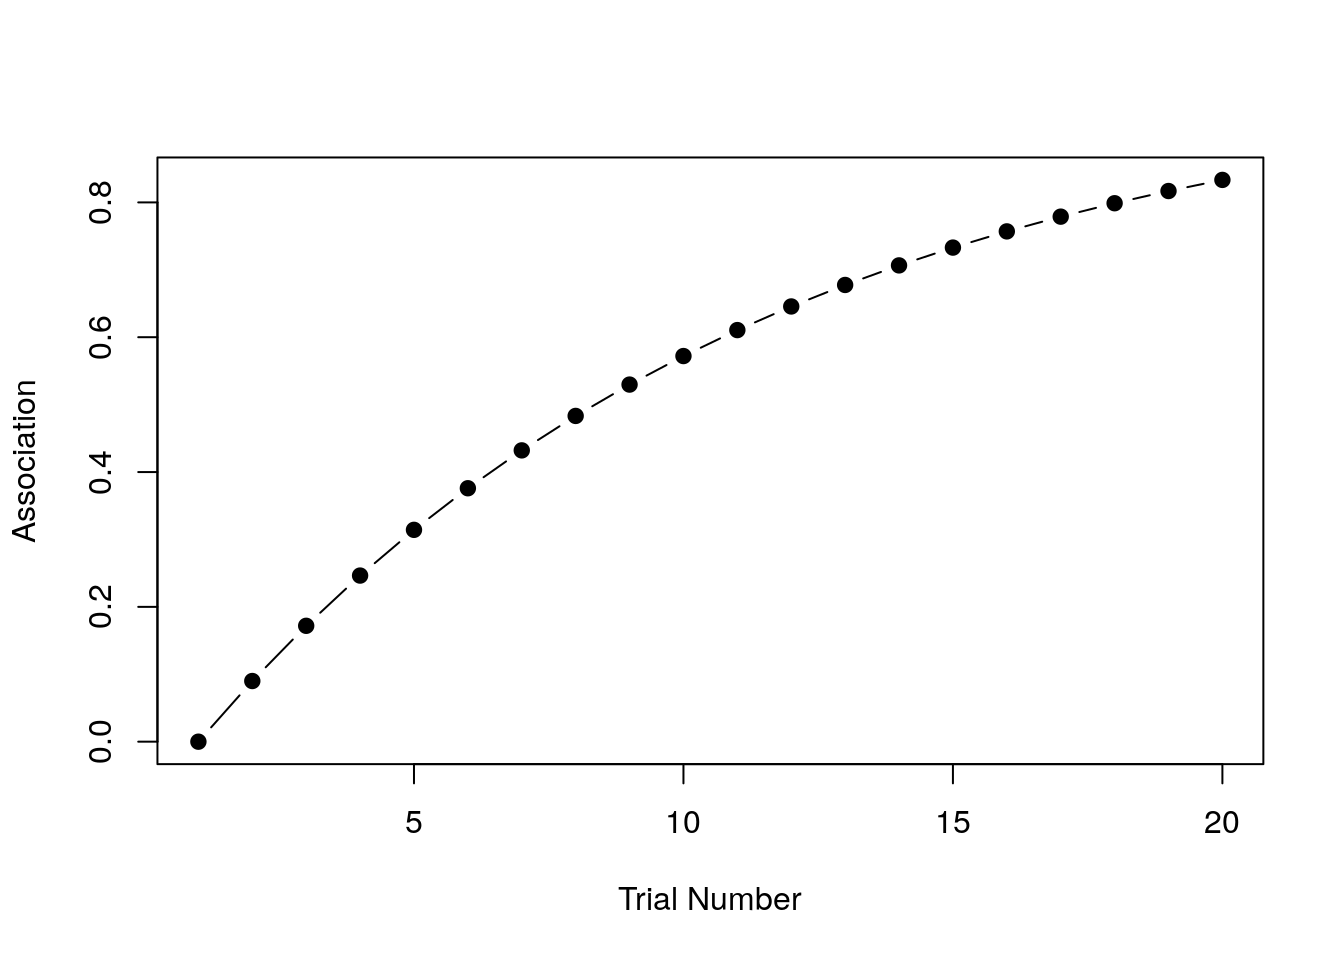
\includegraphics{5-02-programming_files/figure-latex/unnamed-chunk-34-1.pdf}

I've hidden the R command that produces the plot, because we haven't covered data visualisation yet. However, if you are interested in a sneak peek, the source code for all the analyses in this section are \href{./scripts/rescorla_wagner.R}{here}.

\hypertarget{extinction}{%
\subsection{Extinction}\label{extinction}}

For the second example, let's consider the extinction of a learned association. What we'll do this time is start out doing the same thing as last time. For the first 25 trials we'll present a CS-US trial that pairs a tone with a shock (or whatever) and over that time the association for the CS will rise to match the reward ``value'' (\(\lambda = .3\)) linked to the US. Then for the next 25 trials we will present the CS alone with no US present. We'll capture this by setting \(\lambda = 0\) to reflect the fact that the ``value'' to be predicted is now zero (i.e.~no shock). For simplicity, we'll leave the learning rate \(\beta\) the same for shock and no-shock.

Okay here goes. First, let's set up our variables:

\begin{Shaded}
\begin{Highlighting}[]
\NormalTok{n_trials <-}\StringTok{ }\DecValTok{50}                
\NormalTok{strength <-}\StringTok{ }\KeywordTok{numeric}\NormalTok{(n_trials) }
\NormalTok{lambda <-}\StringTok{ }\FloatTok{.3} \CommentTok{# initial reward value }
\end{Highlighting}
\end{Shaded}

Now we have to set up our loop, same as before. This time around we need to include an \texttt{if} statement in the loop, to check whether we have moved from the learning phase (trials 1 to 25) to the extinction phase (trials 26 to 50), and adjust the value of \(\lambda\) accordingly.

\begin{Shaded}
\begin{Highlighting}[]
\ControlFlowTok{for}\NormalTok{(trial }\ControlFlowTok{in} \DecValTok{2}\OperatorTok{:}\NormalTok{n_trials) \{}
  
  \CommentTok{# remove the shock after trial 25}
  \ControlFlowTok{if}\NormalTok{(trial }\OperatorTok{>}\StringTok{ }\DecValTok{25}\NormalTok{) \{}
\NormalTok{    lambda <-}\StringTok{ }\DecValTok{0}
\NormalTok{  \}}
  
  \CommentTok{# update associative strength on each trial}
\NormalTok{  strength[trial] <-}\StringTok{ }\KeywordTok{update_RW}\NormalTok{(}
    \DataTypeTok{value =}\NormalTok{ strength[trial}\DecValTok{-1}\NormalTok{],}
    \DataTypeTok{lambda =}\NormalTok{ lambda}
\NormalTok{  )}
\NormalTok{\}}
\end{Highlighting}
\end{Shaded}

What we expect to see in this situation is that after trial 25 when the shock is removed, the association strength starts to weaken because the learner is now associating the CS with no-shock (i.e. \(\lambda\) has dropped to zero and so the association \(v\) is slowly reverting to that value). Here's the raw numbers:

\begin{Shaded}
\begin{Highlighting}[]
\KeywordTok{print}\NormalTok{(strength)}
\end{Highlighting}
\end{Shaded}

\begin{verbatim}
##  [1] 0.00000000 0.02700000 0.05157000 0.07392870 0.09427512 0.11279036
##  [7] 0.12963922 0.14497169 0.15892424 0.17162106 0.18317516 0.19368940
## [13] 0.20325735 0.21196419 0.21988741 0.22709755 0.23365877 0.23962948
## [19] 0.24506283 0.25000717 0.25450653 0.25860094 0.26232685 0.26571744
## [25] 0.26880287 0.24461061 0.22259565 0.20256205 0.18433146 0.16774163
## [31] 0.15264488 0.13890684 0.12640523 0.11502876 0.10467617 0.09525531
## [37] 0.08668234 0.07888093 0.07178164 0.06532129 0.05944238 0.05409256
## [43] 0.04922423 0.04479405 0.04076259 0.03709395 0.03375550 0.03071750
## [49] 0.02795293 0.02543716
\end{verbatim}

Here they are as a pretty picture:

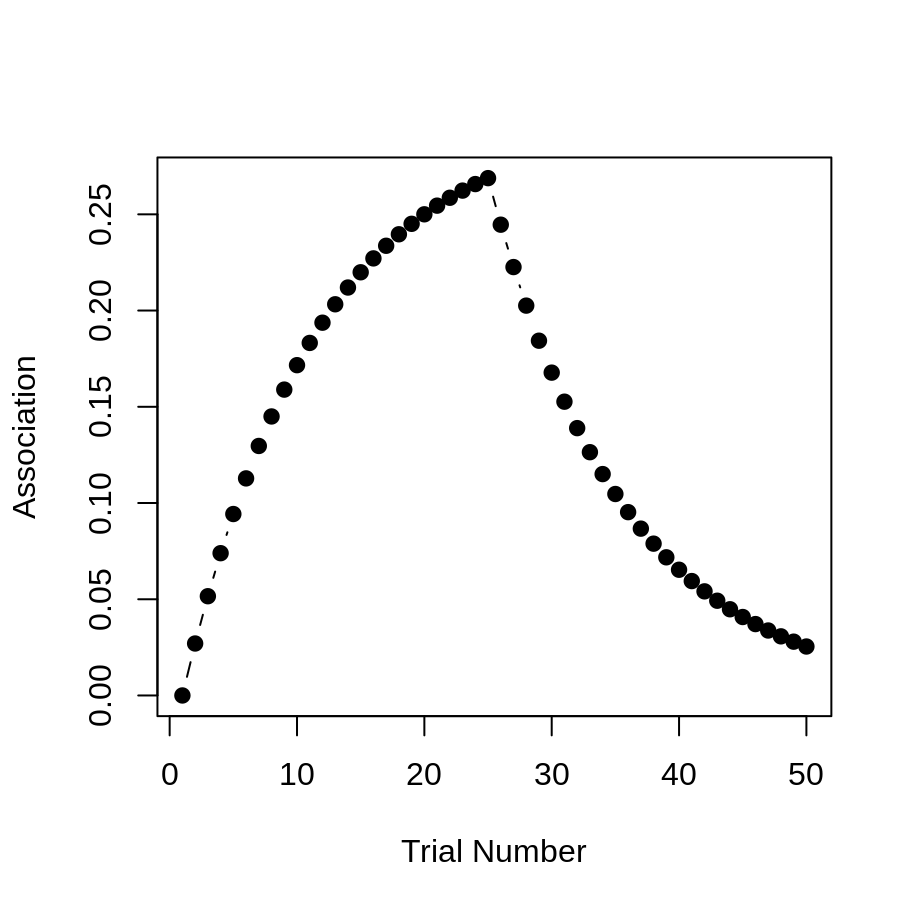
\includegraphics{5-02-programming_files/figure-latex/unnamed-chunk-38-1.pdf}

That looks right to me! Extinction is initially effective at removing the association, but it's effectiveness declines over time, so that by the end of the task there's still some association left.

\hypertarget{blocking}{%
\subsection{Blocking}\label{blocking}}

For the final example, consider a blocking paradigm. In this design we might initially pair a tone with a shock (A+ trials) for a number of trials until an association is learned. Then we present a compound stimulus AB (tone plus light) together with a shock (AB+). During the first phase, the learner quickly acquires a strong association between A and the shock, but then during the second phase they don't learn very much about B, because A already predicts the shock.\footnote{In a real blocking study there would be various control conditions but I'm not going to bother modelling those here. I just want to show how our code works for the important one!}

Because we are presenting a compound stimulus, the values that we pass to the \texttt{update\_RW} function can be vectors. But that's okay, we designed our function to be able to handle that. So let's start by setting up our modelling exercise:

\begin{Shaded}
\begin{Highlighting}[]
\CommentTok{# total number of trials across }
\CommentTok{# both phases of the task}
\NormalTok{n_trials <-}\StringTok{ }\DecValTok{50}

\CommentTok{# vectors of zeros}
\NormalTok{strength_A <-}\StringTok{ }\KeywordTok{rep}\NormalTok{(}\DecValTok{0}\NormalTok{,n_trials)}
\NormalTok{strength_B <-}\StringTok{ }\KeywordTok{rep}\NormalTok{(}\DecValTok{0}\NormalTok{,n_trials)}
\end{Highlighting}
\end{Shaded}

There are two strength vectors here, one for the tone (A) and one for the light (B). Of course, during the first phase of the task the light isn't actually present, which we can capture by setting the relevant learning rate (or salience) parameter \(\alpha\) to 0:

\begin{Shaded}
\begin{Highlighting}[]
\NormalTok{alpha <-}\StringTok{ }\KeywordTok{c}\NormalTok{(.}\DecValTok{3}\NormalTok{, }\DecValTok{0}\NormalTok{)}
\end{Highlighting}
\end{Shaded}

This means that at the start of the task, the model will learn about the tone but not the light. After trial 15, however, both stimuli will be present. For simplicity I'll assume they're equally salient, so after trial 15 the \(\alpha\) value becomes .3 for both stimuli.

As before we construct a loop over the trials:

\begin{Shaded}
\begin{Highlighting}[]
\ControlFlowTok{for}\NormalTok{(trial }\ControlFlowTok{in} \DecValTok{2}\OperatorTok{:}\NormalTok{n_trials) \{}
  
  \CommentTok{# after trial 15, both stimuli are present}
  \ControlFlowTok{if}\NormalTok{(trial }\OperatorTok{>}\StringTok{ }\DecValTok{15}\NormalTok{) alpha <-}\StringTok{ }\KeywordTok{c}\NormalTok{(.}\DecValTok{3}\NormalTok{, }\FloatTok{.3}\NormalTok{)}
  
  \CommentTok{# vector of current associative strengths}
\NormalTok{  v_old <-}\StringTok{ }\KeywordTok{c}\NormalTok{(strength_A[trial}\DecValTok{-1}\NormalTok{], strength_B[trial}\DecValTok{-1}\NormalTok{])}
  
  \CommentTok{# vector of new associative strengths}
\NormalTok{  v_new <-}\StringTok{ }\KeywordTok{update_RW}\NormalTok{(}
    \DataTypeTok{value =}\NormalTok{ v_old,}
    \DataTypeTok{alpha =}\NormalTok{ alpha}
\NormalTok{   )}
  
  \CommentTok{# record the new strengths}
\NormalTok{  strength_A[trial] <-}\StringTok{ }\NormalTok{v_new[}\DecValTok{1}\NormalTok{]}
\NormalTok{  strength_B[trial] <-}\StringTok{ }\NormalTok{v_new[}\DecValTok{2}\NormalTok{]}
\NormalTok{\}}
\end{Highlighting}
\end{Shaded}

It's a little more complex this time because we have read off two strength values and pass them to the \texttt{update\_RW} function.\footnote{In fact, we could make this code a lot simpler if we'd recorded the strengths as a \textbf{matrix} rather than two vectors, but since I haven't introduced matrices yet I've left it in this slightly more clunky form with vectors} Hopefully it is clear what this code is doing.

As with the previous two examples we could print out \texttt{strength\_A} and \texttt{strength\_B}, but realistically no-one likes looking at long lists of numbers so let's just draw the picture. In the plot below, the blue line shows the associative strength to A and the red line shows the associative strength to B:

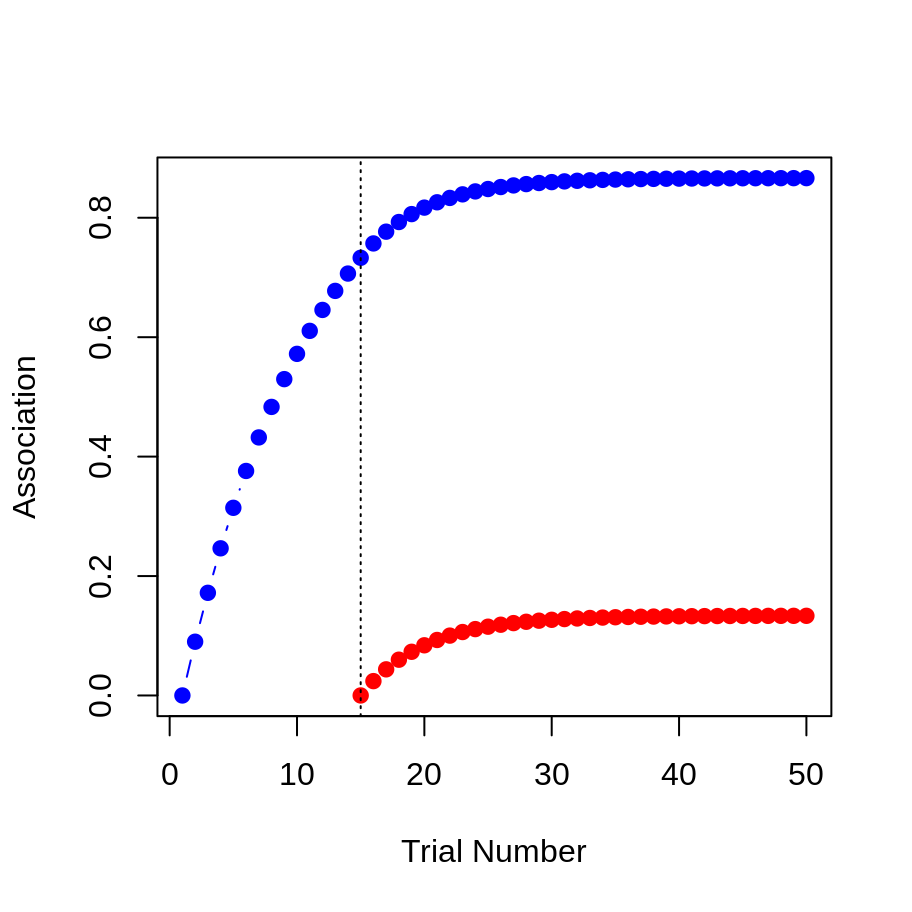
\includegraphics{5-02-programming_files/figure-latex/unnamed-chunk-42-1.pdf}

That's the blocking effect, right there! The model learns a strong association between the tone and the shock (blue) but the association it learns between the light and the shock (red) is much weaker.

\hypertarget{done}{%
\subsection{Done!}\label{done}}

If you've been following along yourself you are now officially a computational modeller. Nice work!

\bibliography{book.bib,packages.bib}


\end{document}
